\documentclass{article}

\usepackage[margin=15mm]{geometry}

\usepackage{multicol}

\usepackage{tikz,paralist}
\usetikzlibrary{
  calc,shapes.multipart,chains,positioning,shadows,
  arrows,arrows.meta,matrix,
  decorations.pathreplacing
}

\begin{document}

\begin{multicols}{3}\raggedcolumns

\begin{enumerate}

\item[$\bullet$] Initial position

\begin{center}

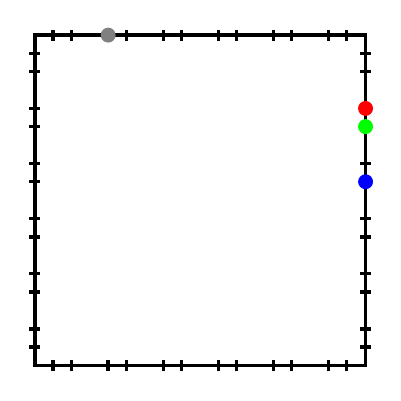
\begin{tikzpicture}[x=7mm,y=7mm]

\draw[very thick] (0.000000,0.000000) rectangle (6.000000,-6.000000);
\draw (0.000000,0.000000) grid[step=6] (6.000000,-6.000000);
\draw[very thick] (-0.100000,-0.330000) to (0.100000,-0.330000);
\draw[very thick] (5.900000,-0.330000) to (6.100000,-0.330000);
\draw[very thick] (0.330000,-0.100000) to (0.330000,0.100000);
\draw[very thick] (0.330000,-6.100000) to (0.330000,-5.900000);
\draw[very thick] (-0.100000,-0.660000) to (0.100000,-0.660000);
\draw[very thick] (5.900000,-0.660000) to (6.100000,-0.660000);
\draw[very thick] (0.660000,-0.100000) to (0.660000,0.100000);
\draw[very thick] (0.660000,-6.100000) to (0.660000,-5.900000);
\draw[very thick] (-0.100000,-1.330000) to (0.100000,-1.330000);
\draw[very thick] (5.900000,-1.330000) to (6.100000,-1.330000);
\draw[very thick] (1.330000,-0.100000) to (1.330000,0.100000);
\draw[very thick] (1.330000,-6.100000) to (1.330000,-5.900000);
\draw[very thick] (-0.100000,-1.660000) to (0.100000,-1.660000);
\draw[very thick] (5.900000,-1.660000) to (6.100000,-1.660000);
\draw[very thick] (1.660000,-0.100000) to (1.660000,0.100000);
\draw[very thick] (1.660000,-6.100000) to (1.660000,-5.900000);
\draw[very thick] (-0.100000,-2.330000) to (0.100000,-2.330000);
\draw[very thick] (5.900000,-2.330000) to (6.100000,-2.330000);
\draw[very thick] (2.330000,-0.100000) to (2.330000,0.100000);
\draw[very thick] (2.330000,-6.100000) to (2.330000,-5.900000);
\draw[very thick] (-0.100000,-2.660000) to (0.100000,-2.660000);
\draw[very thick] (5.900000,-2.660000) to (6.100000,-2.660000);
\draw[very thick] (2.660000,-0.100000) to (2.660000,0.100000);
\draw[very thick] (2.660000,-6.100000) to (2.660000,-5.900000);
\draw[very thick] (-0.100000,-3.330000) to (0.100000,-3.330000);
\draw[very thick] (5.900000,-3.330000) to (6.100000,-3.330000);
\draw[very thick] (3.330000,-0.100000) to (3.330000,0.100000);
\draw[very thick] (3.330000,-6.100000) to (3.330000,-5.900000);
\draw[very thick] (-0.100000,-3.660000) to (0.100000,-3.660000);
\draw[very thick] (5.900000,-3.660000) to (6.100000,-3.660000);
\draw[very thick] (3.660000,-0.100000) to (3.660000,0.100000);
\draw[very thick] (3.660000,-6.100000) to (3.660000,-5.900000);
\draw[very thick] (-0.100000,-4.330000) to (0.100000,-4.330000);
\draw[very thick] (5.900000,-4.330000) to (6.100000,-4.330000);
\draw[very thick] (4.330000,-0.100000) to (4.330000,0.100000);
\draw[very thick] (4.330000,-6.100000) to (4.330000,-5.900000);
\draw[very thick] (-0.100000,-4.660000) to (0.100000,-4.660000);
\draw[very thick] (5.900000,-4.660000) to (6.100000,-4.660000);
\draw[very thick] (4.660000,-0.100000) to (4.660000,0.100000);
\draw[very thick] (4.660000,-6.100000) to (4.660000,-5.900000);
\draw[very thick] (-0.100000,-5.330000) to (0.100000,-5.330000);
\draw[very thick] (5.900000,-5.330000) to (6.100000,-5.330000);
\draw[very thick] (5.330000,-0.100000) to (5.330000,0.100000);
\draw[very thick] (5.330000,-6.100000) to (5.330000,-5.900000);
\draw[very thick] (-0.100000,-5.660000) to (0.100000,-5.660000);
\draw[very thick] (5.900000,-5.660000) to (6.100000,-5.660000);
\draw[very thick] (5.660000,-0.100000) to (5.660000,0.100000);
\draw[very thick] (5.660000,-6.100000) to (5.660000,-5.900000);
\draw[draw=red,fill=red] (6.000000,-1.330000) circle [x radius=0.125000,y radius=0.125000];
\draw[draw=green,fill=green] (6.000000,-1.660000) circle [x radius=0.125000,y radius=0.125000];
\draw[draw=blue,fill=blue] (6.000000,-2.660000) circle [x radius=0.125000,y radius=0.125000];
\draw[draw=gray,fill=gray] (1.330000,0.000000) circle [x radius=0.125000,y radius=0.125000];
\end{tikzpicture}

\end{center}

\item[(1)] Player 1 \textcolor{gray}{\LARGE$\bullet$} draws 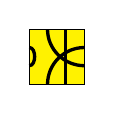
\begin{tikzpicture}[x=7mm,y=7mm]

\draw[black,fill=yellow] (0.000000,0.000000) rectangle (1.000000,-1.000000);
\draw[out=-90,in=180,looseness=1,very thick] (0.330000,0.000000) to (1.000000,-0.660000);
\draw[out=-90,in=90,looseness=1,very thick] (0.660000,0.000000) to (0.660000,-1.000000);
\draw[out=180,in=90,looseness=1,very thick] (1.000000,-0.330000) to (0.330000,-1.000000);
\draw[out=0,in=0,looseness=1,very thick] (0.000000,-0.660000) to (0.000000,-0.330000);
\end{tikzpicture}

\item[(2)] Player 3 \textcolor{green}{\LARGE$\bullet$} draws 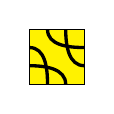
\begin{tikzpicture}[x=7mm,y=7mm]

\draw[black,fill=yellow] (0.000000,0.000000) rectangle (1.000000,-1.000000);
\draw[out=-90,in=180,looseness=1,very thick] (0.330000,0.000000) to (1.000000,-0.330000);
\draw[out=-90,in=180,looseness=1,very thick] (0.660000,0.000000) to (1.000000,-0.660000);
\draw[out=90,in=0,looseness=1,very thick] (0.660000,-1.000000) to (0.000000,-0.660000);
\draw[out=90,in=0,looseness=1,very thick] (0.330000,-1.000000) to (0.000000,-0.330000);
\end{tikzpicture}

\item[(3)] Player 2 \textcolor{blue}{\LARGE$\bullet$} draws 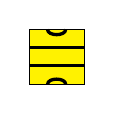
\begin{tikzpicture}[x=7mm,y=7mm]

\draw[black,fill=yellow] (0.000000,0.000000) rectangle (1.000000,-1.000000);
\draw[out=-90,in=-90,looseness=1,very thick] (0.330000,0.000000) to (0.660000,0.000000);
\draw[out=180,in=0,looseness=1,very thick] (1.000000,-0.330000) to (0.000000,-0.330000);
\draw[out=180,in=0,looseness=1,very thick] (1.000000,-0.660000) to (0.000000,-0.660000);
\draw[out=90,in=90,looseness=1,very thick] (0.660000,-1.000000) to (0.330000,-1.000000);
\end{tikzpicture}

\item[(4)] Player 4 \textcolor{red}{\LARGE$\bullet$} draws 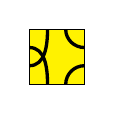
\begin{tikzpicture}[x=7mm,y=7mm]

\draw[black,fill=yellow] (0.000000,0.000000) rectangle (1.000000,-1.000000);
\draw[out=-90,in=0,looseness=1,very thick] (0.330000,0.000000) to (0.000000,-0.660000);
\draw[out=-90,in=180,looseness=1,very thick] (0.660000,0.000000) to (1.000000,-0.330000);
\draw[out=180,in=90,looseness=1,very thick] (1.000000,-0.660000) to (0.660000,-1.000000);
\draw[out=90,in=0,looseness=1,very thick] (0.330000,-1.000000) to (0.000000,-0.330000);
\end{tikzpicture}

\item[(5)] Player 1 \textcolor{gray}{\LARGE$\bullet$} draws 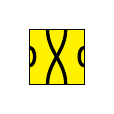
\begin{tikzpicture}[x=7mm,y=7mm]

\draw[black,fill=yellow] (0.000000,0.000000) rectangle (1.000000,-1.000000);
\draw[out=-90,in=90,looseness=1,very thick] (0.330000,0.000000) to (0.660000,-1.000000);
\draw[out=-90,in=90,looseness=1,very thick] (0.660000,0.000000) to (0.330000,-1.000000);
\draw[out=180,in=180,looseness=1,very thick] (1.000000,-0.330000) to (1.000000,-0.660000);
\draw[out=0,in=0,looseness=1,very thick] (0.000000,-0.660000) to (0.000000,-0.330000);
\end{tikzpicture}

\item[(6)] Player 3 \textcolor{green}{\LARGE$\bullet$} draws 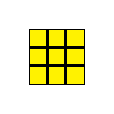
\begin{tikzpicture}[x=7mm,y=7mm]

\draw[black,fill=yellow] (0.000000,0.000000) rectangle (1.000000,-1.000000);
\draw[out=-90,in=90,looseness=1,very thick] (0.330000,0.000000) to (0.330000,-1.000000);
\draw[out=-90,in=90,looseness=1,very thick] (0.660000,0.000000) to (0.660000,-1.000000);
\draw[out=180,in=0,looseness=1,very thick] (1.000000,-0.330000) to (0.000000,-0.330000);
\draw[out=180,in=0,looseness=1,very thick] (1.000000,-0.660000) to (0.000000,-0.660000);
\end{tikzpicture}

\item[(7)] Player 2 \textcolor{blue}{\LARGE$\bullet$} draws 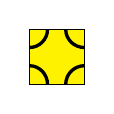
\begin{tikzpicture}[x=7mm,y=7mm]

\draw[black,fill=yellow] (0.000000,0.000000) rectangle (1.000000,-1.000000);
\draw[out=-90,in=0,looseness=1,very thick] (0.330000,0.000000) to (0.000000,-0.330000);
\draw[out=-90,in=180,looseness=1,very thick] (0.660000,0.000000) to (1.000000,-0.330000);
\draw[out=180,in=90,looseness=1,very thick] (1.000000,-0.660000) to (0.660000,-1.000000);
\draw[out=90,in=0,looseness=1,very thick] (0.330000,-1.000000) to (0.000000,-0.660000);
\end{tikzpicture}

\item[(8)] Player 4 \textcolor{red}{\LARGE$\bullet$} draws 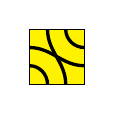
\begin{tikzpicture}[x=7mm,y=7mm]

\draw[black,fill=yellow] (0.000000,0.000000) rectangle (1.000000,-1.000000);
\draw[out=-90,in=90,looseness=1,very thick] (0.330000,0.000000) to (0.660000,-1.000000);
\draw[out=-90,in=180,looseness=1,very thick] (0.660000,0.000000) to (1.000000,-0.330000);
\draw[out=180,in=0,looseness=1,very thick] (1.000000,-0.660000) to (0.000000,-0.330000);
\draw[out=90,in=0,looseness=1,very thick] (0.330000,-1.000000) to (0.000000,-0.660000);
\end{tikzpicture}

\item[(9)] Player 1 \textcolor{gray}{\LARGE$\bullet$} draws 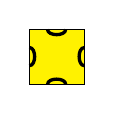
\begin{tikzpicture}[x=7mm,y=7mm]

\draw[black,fill=yellow] (0.000000,0.000000) rectangle (1.000000,-1.000000);
\draw[out=-90,in=-90,looseness=1,very thick] (0.330000,0.000000) to (0.660000,0.000000);
\draw[out=180,in=180,looseness=1,very thick] (1.000000,-0.330000) to (1.000000,-0.660000);
\draw[out=90,in=90,looseness=1,very thick] (0.660000,-1.000000) to (0.330000,-1.000000);
\draw[out=0,in=0,looseness=1,very thick] (0.000000,-0.660000) to (0.000000,-0.330000);
\end{tikzpicture}

\item[(10)] Player 3 \textcolor{green}{\LARGE$\bullet$} draws 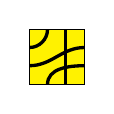
\begin{tikzpicture}[x=7mm,y=7mm]

\draw[black,fill=yellow] (0.000000,0.000000) rectangle (1.000000,-1.000000);
\draw[out=-90,in=0,looseness=1,very thick] (0.330000,0.000000) to (0.000000,-0.330000);
\draw[out=-90,in=90,looseness=1,very thick] (0.660000,0.000000) to (0.660000,-1.000000);
\draw[out=180,in=0,looseness=1,very thick] (1.000000,-0.330000) to (0.000000,-0.660000);
\draw[out=180,in=90,looseness=1,very thick] (1.000000,-0.660000) to (0.330000,-1.000000);
\end{tikzpicture}

\item[(11)] Player 2 \textcolor{blue}{\LARGE$\bullet$} draws 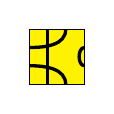
\begin{tikzpicture}[x=7mm,y=7mm]

\draw[black,fill=yellow] (0.000000,0.000000) rectangle (1.000000,-1.000000);
\draw[out=-90,in=90,looseness=1,very thick] (0.330000,0.000000) to (0.330000,-1.000000);
\draw[out=-90,in=0,looseness=1,very thick] (0.660000,0.000000) to (0.000000,-0.330000);
\draw[out=180,in=180,looseness=1,very thick] (1.000000,-0.330000) to (1.000000,-0.660000);
\draw[out=90,in=0,looseness=1,very thick] (0.660000,-1.000000) to (0.000000,-0.660000);
\end{tikzpicture}

\item[(12)] Player 4 \textcolor{red}{\LARGE$\bullet$} draws 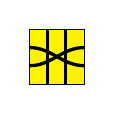
\begin{tikzpicture}[x=7mm,y=7mm]

\draw[black,fill=yellow] (0.000000,0.000000) rectangle (1.000000,-1.000000);
\draw[out=-90,in=90,looseness=1,very thick] (0.330000,0.000000) to (0.330000,-1.000000);
\draw[out=-90,in=90,looseness=1,very thick] (0.660000,0.000000) to (0.660000,-1.000000);
\draw[out=180,in=0,looseness=1,very thick] (1.000000,-0.330000) to (0.000000,-0.660000);
\draw[out=180,in=0,looseness=1,very thick] (1.000000,-0.660000) to (0.000000,-0.330000);
\end{tikzpicture}

\item Player 1 \textcolor{gray}{\LARGE$\bullet$} plays at row 1, col 2:
\begin{center}

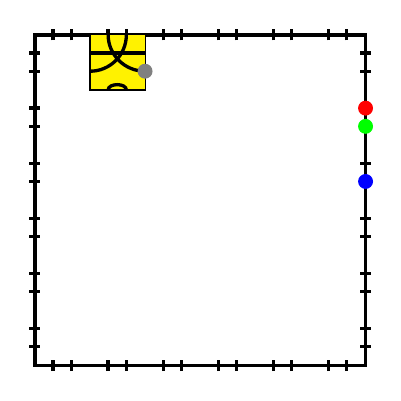
\begin{tikzpicture}[x=7mm,y=7mm]

\draw[very thick] (0.000000,0.000000) rectangle (6.000000,-6.000000);
\draw (0.000000,0.000000) grid[step=6] (6.000000,-6.000000);
\draw[very thick] (-0.100000,-0.330000) to (0.100000,-0.330000);
\draw[very thick] (5.900000,-0.330000) to (6.100000,-0.330000);
\draw[very thick] (0.330000,-0.100000) to (0.330000,0.100000);
\draw[very thick] (0.330000,-6.100000) to (0.330000,-5.900000);
\draw[very thick] (-0.100000,-0.660000) to (0.100000,-0.660000);
\draw[very thick] (5.900000,-0.660000) to (6.100000,-0.660000);
\draw[very thick] (0.660000,-0.100000) to (0.660000,0.100000);
\draw[very thick] (0.660000,-6.100000) to (0.660000,-5.900000);
\draw[very thick] (-0.100000,-1.330000) to (0.100000,-1.330000);
\draw[very thick] (5.900000,-1.330000) to (6.100000,-1.330000);
\draw[very thick] (1.330000,-0.100000) to (1.330000,0.100000);
\draw[very thick] (1.330000,-6.100000) to (1.330000,-5.900000);
\draw[very thick] (-0.100000,-1.660000) to (0.100000,-1.660000);
\draw[very thick] (5.900000,-1.660000) to (6.100000,-1.660000);
\draw[very thick] (1.660000,-0.100000) to (1.660000,0.100000);
\draw[very thick] (1.660000,-6.100000) to (1.660000,-5.900000);
\draw[very thick] (-0.100000,-2.330000) to (0.100000,-2.330000);
\draw[very thick] (5.900000,-2.330000) to (6.100000,-2.330000);
\draw[very thick] (2.330000,-0.100000) to (2.330000,0.100000);
\draw[very thick] (2.330000,-6.100000) to (2.330000,-5.900000);
\draw[very thick] (-0.100000,-2.660000) to (0.100000,-2.660000);
\draw[very thick] (5.900000,-2.660000) to (6.100000,-2.660000);
\draw[very thick] (2.660000,-0.100000) to (2.660000,0.100000);
\draw[very thick] (2.660000,-6.100000) to (2.660000,-5.900000);
\draw[very thick] (-0.100000,-3.330000) to (0.100000,-3.330000);
\draw[very thick] (5.900000,-3.330000) to (6.100000,-3.330000);
\draw[very thick] (3.330000,-0.100000) to (3.330000,0.100000);
\draw[very thick] (3.330000,-6.100000) to (3.330000,-5.900000);
\draw[very thick] (-0.100000,-3.660000) to (0.100000,-3.660000);
\draw[very thick] (5.900000,-3.660000) to (6.100000,-3.660000);
\draw[very thick] (3.660000,-0.100000) to (3.660000,0.100000);
\draw[very thick] (3.660000,-6.100000) to (3.660000,-5.900000);
\draw[very thick] (-0.100000,-4.330000) to (0.100000,-4.330000);
\draw[very thick] (5.900000,-4.330000) to (6.100000,-4.330000);
\draw[very thick] (4.330000,-0.100000) to (4.330000,0.100000);
\draw[very thick] (4.330000,-6.100000) to (4.330000,-5.900000);
\draw[very thick] (-0.100000,-4.660000) to (0.100000,-4.660000);
\draw[very thick] (5.900000,-4.660000) to (6.100000,-4.660000);
\draw[very thick] (4.660000,-0.100000) to (4.660000,0.100000);
\draw[very thick] (4.660000,-6.100000) to (4.660000,-5.900000);
\draw[very thick] (-0.100000,-5.330000) to (0.100000,-5.330000);
\draw[very thick] (5.900000,-5.330000) to (6.100000,-5.330000);
\draw[very thick] (5.330000,-0.100000) to (5.330000,0.100000);
\draw[very thick] (5.330000,-6.100000) to (5.330000,-5.900000);
\draw[very thick] (-0.100000,-5.660000) to (0.100000,-5.660000);
\draw[very thick] (5.900000,-5.660000) to (6.100000,-5.660000);
\draw[very thick] (5.660000,-0.100000) to (5.660000,0.100000);
\draw[very thick] (5.660000,-6.100000) to (5.660000,-5.900000);
\draw[black,fill=yellow] (1.000000,0.000000) rectangle (2.000000,-1.000000);
\draw[out=-90,in=180,looseness=1,very thick] (1.330000,0.000000) to (2.000000,-0.660000);
\draw[out=-90,in=0,looseness=1,very thick] (1.660000,0.000000) to (1.000000,-0.660000);
\draw[out=180,in=0,looseness=1,very thick] (2.000000,-0.330000) to (1.000000,-0.330000);
\draw[out=90,in=90,looseness=1,very thick] (1.660000,-1.000000) to (1.330000,-1.000000);
\draw[draw=red,fill=red] (6.000000,-1.330000) circle [x radius=0.125000,y radius=0.125000];
\draw[draw=green,fill=green] (6.000000,-1.660000) circle [x radius=0.125000,y radius=0.125000];
\draw[draw=blue,fill=blue] (6.000000,-2.660000) circle [x radius=0.125000,y radius=0.125000];
\draw[draw=gray,fill=gray] (2.000000,-0.660000) circle [x radius=0.125000,y radius=0.125000];
\end{tikzpicture}

\end{center}

\item[(13)] Player 1 \textcolor{gray}{\LARGE$\bullet$} draws 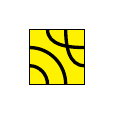
\begin{tikzpicture}[x=7mm,y=7mm]

\draw[black,fill=yellow] (0.000000,0.000000) rectangle (1.000000,-1.000000);
\draw[out=-90,in=180,looseness=1,very thick] (0.330000,0.000000) to (1.000000,-0.330000);
\draw[out=-90,in=180,looseness=1,very thick] (0.660000,0.000000) to (1.000000,-0.660000);
\draw[out=90,in=0,looseness=1,very thick] (0.660000,-1.000000) to (0.000000,-0.330000);
\draw[out=90,in=0,looseness=1,very thick] (0.330000,-1.000000) to (0.000000,-0.660000);
\end{tikzpicture}

\item Player 3 \textcolor{green}{\LARGE$\bullet$} plays at row 2, col 6:
\begin{center}

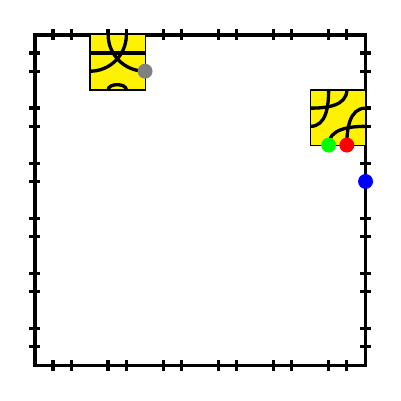
\begin{tikzpicture}[x=7mm,y=7mm]

\draw[very thick] (0.000000,0.000000) rectangle (6.000000,-6.000000);
\draw (0.000000,0.000000) grid[step=6] (6.000000,-6.000000);
\draw[very thick] (-0.100000,-0.330000) to (0.100000,-0.330000);
\draw[very thick] (5.900000,-0.330000) to (6.100000,-0.330000);
\draw[very thick] (0.330000,-0.100000) to (0.330000,0.100000);
\draw[very thick] (0.330000,-6.100000) to (0.330000,-5.900000);
\draw[very thick] (-0.100000,-0.660000) to (0.100000,-0.660000);
\draw[very thick] (5.900000,-0.660000) to (6.100000,-0.660000);
\draw[very thick] (0.660000,-0.100000) to (0.660000,0.100000);
\draw[very thick] (0.660000,-6.100000) to (0.660000,-5.900000);
\draw[very thick] (-0.100000,-1.330000) to (0.100000,-1.330000);
\draw[very thick] (5.900000,-1.330000) to (6.100000,-1.330000);
\draw[very thick] (1.330000,-0.100000) to (1.330000,0.100000);
\draw[very thick] (1.330000,-6.100000) to (1.330000,-5.900000);
\draw[very thick] (-0.100000,-1.660000) to (0.100000,-1.660000);
\draw[very thick] (5.900000,-1.660000) to (6.100000,-1.660000);
\draw[very thick] (1.660000,-0.100000) to (1.660000,0.100000);
\draw[very thick] (1.660000,-6.100000) to (1.660000,-5.900000);
\draw[very thick] (-0.100000,-2.330000) to (0.100000,-2.330000);
\draw[very thick] (5.900000,-2.330000) to (6.100000,-2.330000);
\draw[very thick] (2.330000,-0.100000) to (2.330000,0.100000);
\draw[very thick] (2.330000,-6.100000) to (2.330000,-5.900000);
\draw[very thick] (-0.100000,-2.660000) to (0.100000,-2.660000);
\draw[very thick] (5.900000,-2.660000) to (6.100000,-2.660000);
\draw[very thick] (2.660000,-0.100000) to (2.660000,0.100000);
\draw[very thick] (2.660000,-6.100000) to (2.660000,-5.900000);
\draw[very thick] (-0.100000,-3.330000) to (0.100000,-3.330000);
\draw[very thick] (5.900000,-3.330000) to (6.100000,-3.330000);
\draw[very thick] (3.330000,-0.100000) to (3.330000,0.100000);
\draw[very thick] (3.330000,-6.100000) to (3.330000,-5.900000);
\draw[very thick] (-0.100000,-3.660000) to (0.100000,-3.660000);
\draw[very thick] (5.900000,-3.660000) to (6.100000,-3.660000);
\draw[very thick] (3.660000,-0.100000) to (3.660000,0.100000);
\draw[very thick] (3.660000,-6.100000) to (3.660000,-5.900000);
\draw[very thick] (-0.100000,-4.330000) to (0.100000,-4.330000);
\draw[very thick] (5.900000,-4.330000) to (6.100000,-4.330000);
\draw[very thick] (4.330000,-0.100000) to (4.330000,0.100000);
\draw[very thick] (4.330000,-6.100000) to (4.330000,-5.900000);
\draw[very thick] (-0.100000,-4.660000) to (0.100000,-4.660000);
\draw[very thick] (5.900000,-4.660000) to (6.100000,-4.660000);
\draw[very thick] (4.660000,-0.100000) to (4.660000,0.100000);
\draw[very thick] (4.660000,-6.100000) to (4.660000,-5.900000);
\draw[very thick] (-0.100000,-5.330000) to (0.100000,-5.330000);
\draw[very thick] (5.900000,-5.330000) to (6.100000,-5.330000);
\draw[very thick] (5.330000,-0.100000) to (5.330000,0.100000);
\draw[very thick] (5.330000,-6.100000) to (5.330000,-5.900000);
\draw[very thick] (-0.100000,-5.660000) to (0.100000,-5.660000);
\draw[very thick] (5.900000,-5.660000) to (6.100000,-5.660000);
\draw[very thick] (5.660000,-0.100000) to (5.660000,0.100000);
\draw[very thick] (5.660000,-6.100000) to (5.660000,-5.900000);
\draw[black,fill=yellow] (1.000000,0.000000) rectangle (2.000000,-1.000000);
\draw[out=-90,in=180,looseness=1,very thick] (1.330000,0.000000) to (2.000000,-0.660000);
\draw[out=-90,in=0,looseness=1,very thick] (1.660000,0.000000) to (1.000000,-0.660000);
\draw[out=180,in=0,looseness=1,very thick] (2.000000,-0.330000) to (1.000000,-0.330000);
\draw[out=90,in=90,looseness=1,very thick] (1.660000,-1.000000) to (1.330000,-1.000000);
\draw[black,fill=yellow] (5.000000,-1.000000) rectangle (6.000000,-2.000000);
\draw[out=-90,in=0,looseness=1,very thick] (5.330000,-1.000000) to (5.000000,-1.660000);
\draw[out=-90,in=0,looseness=1,very thick] (5.660000,-1.000000) to (5.000000,-1.330000);
\draw[out=180,in=90,looseness=1,very thick] (6.000000,-1.330000) to (5.660000,-2.000000);
\draw[out=180,in=90,looseness=1,very thick] (6.000000,-1.660000) to (5.330000,-2.000000);
\draw[draw=red,fill=red] (5.660000,-2.000000) circle [x radius=0.125000,y radius=0.125000];
\draw[draw=green,fill=green] (5.330000,-2.000000) circle [x radius=0.125000,y radius=0.125000];
\draw[draw=blue,fill=blue] (6.000000,-2.660000) circle [x radius=0.125000,y radius=0.125000];
\draw[draw=gray,fill=gray] (2.000000,-0.660000) circle [x radius=0.125000,y radius=0.125000];
\end{tikzpicture}

\end{center}

\item[(14)] Player 3 \textcolor{green}{\LARGE$\bullet$} draws 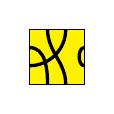
\begin{tikzpicture}[x=7mm,y=7mm]

\draw[black,fill=yellow] (0.000000,0.000000) rectangle (1.000000,-1.000000);
\draw[out=-90,in=90,looseness=1,very thick] (0.330000,0.000000) to (0.660000,-1.000000);
\draw[out=-90,in=0,looseness=1,very thick] (0.660000,0.000000) to (0.000000,-0.660000);
\draw[out=180,in=180,looseness=1,very thick] (1.000000,-0.330000) to (1.000000,-0.660000);
\draw[out=90,in=0,looseness=1,very thick] (0.330000,-1.000000) to (0.000000,-0.330000);
\end{tikzpicture}

\item Player 2 \textcolor{blue}{\LARGE$\bullet$} plays at row 3, col 6:
\begin{center}

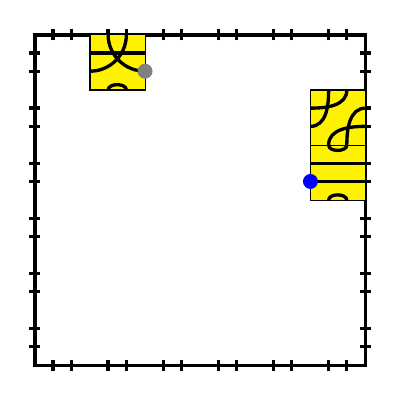
\begin{tikzpicture}[x=7mm,y=7mm]

\draw[very thick] (0.000000,0.000000) rectangle (6.000000,-6.000000);
\draw (0.000000,0.000000) grid[step=6] (6.000000,-6.000000);
\draw[very thick] (-0.100000,-0.330000) to (0.100000,-0.330000);
\draw[very thick] (5.900000,-0.330000) to (6.100000,-0.330000);
\draw[very thick] (0.330000,-0.100000) to (0.330000,0.100000);
\draw[very thick] (0.330000,-6.100000) to (0.330000,-5.900000);
\draw[very thick] (-0.100000,-0.660000) to (0.100000,-0.660000);
\draw[very thick] (5.900000,-0.660000) to (6.100000,-0.660000);
\draw[very thick] (0.660000,-0.100000) to (0.660000,0.100000);
\draw[very thick] (0.660000,-6.100000) to (0.660000,-5.900000);
\draw[very thick] (-0.100000,-1.330000) to (0.100000,-1.330000);
\draw[very thick] (5.900000,-1.330000) to (6.100000,-1.330000);
\draw[very thick] (1.330000,-0.100000) to (1.330000,0.100000);
\draw[very thick] (1.330000,-6.100000) to (1.330000,-5.900000);
\draw[very thick] (-0.100000,-1.660000) to (0.100000,-1.660000);
\draw[very thick] (5.900000,-1.660000) to (6.100000,-1.660000);
\draw[very thick] (1.660000,-0.100000) to (1.660000,0.100000);
\draw[very thick] (1.660000,-6.100000) to (1.660000,-5.900000);
\draw[very thick] (-0.100000,-2.330000) to (0.100000,-2.330000);
\draw[very thick] (5.900000,-2.330000) to (6.100000,-2.330000);
\draw[very thick] (2.330000,-0.100000) to (2.330000,0.100000);
\draw[very thick] (2.330000,-6.100000) to (2.330000,-5.900000);
\draw[very thick] (-0.100000,-2.660000) to (0.100000,-2.660000);
\draw[very thick] (5.900000,-2.660000) to (6.100000,-2.660000);
\draw[very thick] (2.660000,-0.100000) to (2.660000,0.100000);
\draw[very thick] (2.660000,-6.100000) to (2.660000,-5.900000);
\draw[very thick] (-0.100000,-3.330000) to (0.100000,-3.330000);
\draw[very thick] (5.900000,-3.330000) to (6.100000,-3.330000);
\draw[very thick] (3.330000,-0.100000) to (3.330000,0.100000);
\draw[very thick] (3.330000,-6.100000) to (3.330000,-5.900000);
\draw[very thick] (-0.100000,-3.660000) to (0.100000,-3.660000);
\draw[very thick] (5.900000,-3.660000) to (6.100000,-3.660000);
\draw[very thick] (3.660000,-0.100000) to (3.660000,0.100000);
\draw[very thick] (3.660000,-6.100000) to (3.660000,-5.900000);
\draw[very thick] (-0.100000,-4.330000) to (0.100000,-4.330000);
\draw[very thick] (5.900000,-4.330000) to (6.100000,-4.330000);
\draw[very thick] (4.330000,-0.100000) to (4.330000,0.100000);
\draw[very thick] (4.330000,-6.100000) to (4.330000,-5.900000);
\draw[very thick] (-0.100000,-4.660000) to (0.100000,-4.660000);
\draw[very thick] (5.900000,-4.660000) to (6.100000,-4.660000);
\draw[very thick] (4.660000,-0.100000) to (4.660000,0.100000);
\draw[very thick] (4.660000,-6.100000) to (4.660000,-5.900000);
\draw[very thick] (-0.100000,-5.330000) to (0.100000,-5.330000);
\draw[very thick] (5.900000,-5.330000) to (6.100000,-5.330000);
\draw[very thick] (5.330000,-0.100000) to (5.330000,0.100000);
\draw[very thick] (5.330000,-6.100000) to (5.330000,-5.900000);
\draw[very thick] (-0.100000,-5.660000) to (0.100000,-5.660000);
\draw[very thick] (5.900000,-5.660000) to (6.100000,-5.660000);
\draw[very thick] (5.660000,-0.100000) to (5.660000,0.100000);
\draw[very thick] (5.660000,-6.100000) to (5.660000,-5.900000);
\draw[black,fill=yellow] (1.000000,0.000000) rectangle (2.000000,-1.000000);
\draw[out=-90,in=180,looseness=1,very thick] (1.330000,0.000000) to (2.000000,-0.660000);
\draw[out=-90,in=0,looseness=1,very thick] (1.660000,0.000000) to (1.000000,-0.660000);
\draw[out=180,in=0,looseness=1,very thick] (2.000000,-0.330000) to (1.000000,-0.330000);
\draw[out=90,in=90,looseness=1,very thick] (1.660000,-1.000000) to (1.330000,-1.000000);
\draw[black,fill=yellow] (5.000000,-1.000000) rectangle (6.000000,-2.000000);
\draw[out=-90,in=0,looseness=1,very thick] (5.330000,-1.000000) to (5.000000,-1.660000);
\draw[out=-90,in=0,looseness=1,very thick] (5.660000,-1.000000) to (5.000000,-1.330000);
\draw[out=180,in=90,looseness=1,very thick] (6.000000,-1.330000) to (5.660000,-2.000000);
\draw[out=180,in=90,looseness=1,very thick] (6.000000,-1.660000) to (5.330000,-2.000000);
\draw[black,fill=yellow] (5.000000,-2.000000) rectangle (6.000000,-3.000000);
\draw[out=-90,in=-90,looseness=1,very thick] (5.330000,-2.000000) to (5.660000,-2.000000);
\draw[out=180,in=0,looseness=1,very thick] (6.000000,-2.330000) to (5.000000,-2.330000);
\draw[out=180,in=0,looseness=1,very thick] (6.000000,-2.660000) to (5.000000,-2.660000);
\draw[out=90,in=90,looseness=1,very thick] (5.660000,-3.000000) to (5.330000,-3.000000);
\draw[draw=blue,fill=blue] (5.000000,-2.660000) circle [x radius=0.125000,y radius=0.125000];
\draw[draw=gray,fill=gray] (2.000000,-0.660000) circle [x radius=0.125000,y radius=0.125000];
\end{tikzpicture}

\end{center}

\begin{compactitem}

\item Player 4 \textcolor{red}{\LARGE$\bullet$} eliminated.  Returning 3 tiles to deck:\raggedright\ 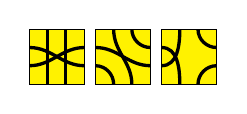
\begin{tikzpicture}[x=7mm,y=7mm]

\draw[black,fill=yellow] (0.000000,0.000000) rectangle (1.000000,-1.000000);
\draw[out=-90,in=90,looseness=1,very thick] (0.330000,0.000000) to (0.330000,-1.000000);
\draw[out=-90,in=90,looseness=1,very thick] (0.660000,0.000000) to (0.660000,-1.000000);
\draw[out=180,in=0,looseness=1,very thick] (1.000000,-0.330000) to (0.000000,-0.660000);
\draw[out=180,in=0,looseness=1,very thick] (1.000000,-0.660000) to (0.000000,-0.330000);
\draw[black,fill=yellow] (1.200000,0.000000) rectangle (2.200000,-1.000000);
\draw[out=-90,in=90,looseness=1,very thick] (1.530000,0.000000) to (1.860000,-1.000000);
\draw[out=-90,in=180,looseness=1,very thick] (1.860000,0.000000) to (2.200000,-0.330000);
\draw[out=180,in=0,looseness=1,very thick] (2.200000,-0.660000) to (1.200000,-0.330000);
\draw[out=90,in=0,looseness=1,very thick] (1.530000,-1.000000) to (1.200000,-0.660000);
\draw[black,fill=yellow] (2.400000,0.000000) rectangle (3.400000,-1.000000);
\draw[out=-90,in=0,looseness=1,very thick] (2.730000,0.000000) to (2.400000,-0.660000);
\draw[out=-90,in=180,looseness=1,very thick] (3.060000,0.000000) to (3.400000,-0.330000);
\draw[out=180,in=90,looseness=1,very thick] (3.400000,-0.660000) to (3.060000,-1.000000);
\draw[out=90,in=0,looseness=1,very thick] (2.730000,-1.000000) to (2.400000,-0.330000);
\end{tikzpicture}

\item Player 3 \textcolor{green}{\LARGE$\bullet$} eliminated.  Returning 3 tiles to deck:\raggedright\ 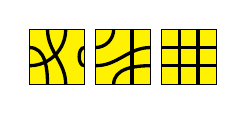
\begin{tikzpicture}[x=7mm,y=7mm]

\draw[black,fill=yellow] (0.000000,0.000000) rectangle (1.000000,-1.000000);
\draw[out=-90,in=90,looseness=1,very thick] (0.330000,0.000000) to (0.660000,-1.000000);
\draw[out=-90,in=0,looseness=1,very thick] (0.660000,0.000000) to (0.000000,-0.660000);
\draw[out=180,in=180,looseness=1,very thick] (1.000000,-0.330000) to (1.000000,-0.660000);
\draw[out=90,in=0,looseness=1,very thick] (0.330000,-1.000000) to (0.000000,-0.330000);
\draw[black,fill=yellow] (1.200000,0.000000) rectangle (2.200000,-1.000000);
\draw[out=-90,in=0,looseness=1,very thick] (1.530000,0.000000) to (1.200000,-0.330000);
\draw[out=-90,in=90,looseness=1,very thick] (1.860000,0.000000) to (1.860000,-1.000000);
\draw[out=180,in=0,looseness=1,very thick] (2.200000,-0.330000) to (1.200000,-0.660000);
\draw[out=180,in=90,looseness=1,very thick] (2.200000,-0.660000) to (1.530000,-1.000000);
\draw[black,fill=yellow] (2.400000,0.000000) rectangle (3.400000,-1.000000);
\draw[out=-90,in=90,looseness=1,very thick] (2.730000,0.000000) to (2.730000,-1.000000);
\draw[out=-90,in=90,looseness=1,very thick] (3.060000,0.000000) to (3.060000,-1.000000);
\draw[out=180,in=0,looseness=1,very thick] (3.400000,-0.330000) to (2.400000,-0.330000);
\draw[out=180,in=0,looseness=1,very thick] (3.400000,-0.660000) to (2.400000,-0.660000);
\end{tikzpicture}

\end{compactitem}

\item[(15)] Player 2 \textcolor{blue}{\LARGE$\bullet$} draws 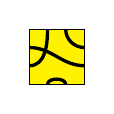
\begin{tikzpicture}[x=7mm,y=7mm]

\draw[black,fill=yellow] (0.000000,0.000000) rectangle (1.000000,-1.000000);
\draw[out=-90,in=0,looseness=1,very thick] (0.330000,0.000000) to (0.000000,-0.660000);
\draw[out=-90,in=180,looseness=1,very thick] (0.660000,0.000000) to (1.000000,-0.330000);
\draw[out=180,in=0,looseness=1,very thick] (1.000000,-0.660000) to (0.000000,-0.330000);
\draw[out=90,in=90,looseness=1,very thick] (0.660000,-1.000000) to (0.330000,-1.000000);
\end{tikzpicture}

\item Player 1 \textcolor{gray}{\LARGE$\bullet$} plays at row 1, col 3:
\begin{center}

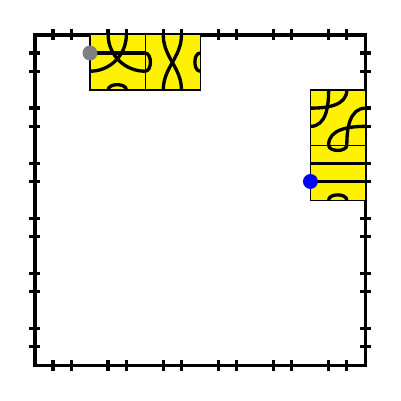
\begin{tikzpicture}[x=7mm,y=7mm]

\draw[very thick] (0.000000,0.000000) rectangle (6.000000,-6.000000);
\draw (0.000000,0.000000) grid[step=6] (6.000000,-6.000000);
\draw[very thick] (-0.100000,-0.330000) to (0.100000,-0.330000);
\draw[very thick] (5.900000,-0.330000) to (6.100000,-0.330000);
\draw[very thick] (0.330000,-0.100000) to (0.330000,0.100000);
\draw[very thick] (0.330000,-6.100000) to (0.330000,-5.900000);
\draw[very thick] (-0.100000,-0.660000) to (0.100000,-0.660000);
\draw[very thick] (5.900000,-0.660000) to (6.100000,-0.660000);
\draw[very thick] (0.660000,-0.100000) to (0.660000,0.100000);
\draw[very thick] (0.660000,-6.100000) to (0.660000,-5.900000);
\draw[very thick] (-0.100000,-1.330000) to (0.100000,-1.330000);
\draw[very thick] (5.900000,-1.330000) to (6.100000,-1.330000);
\draw[very thick] (1.330000,-0.100000) to (1.330000,0.100000);
\draw[very thick] (1.330000,-6.100000) to (1.330000,-5.900000);
\draw[very thick] (-0.100000,-1.660000) to (0.100000,-1.660000);
\draw[very thick] (5.900000,-1.660000) to (6.100000,-1.660000);
\draw[very thick] (1.660000,-0.100000) to (1.660000,0.100000);
\draw[very thick] (1.660000,-6.100000) to (1.660000,-5.900000);
\draw[very thick] (-0.100000,-2.330000) to (0.100000,-2.330000);
\draw[very thick] (5.900000,-2.330000) to (6.100000,-2.330000);
\draw[very thick] (2.330000,-0.100000) to (2.330000,0.100000);
\draw[very thick] (2.330000,-6.100000) to (2.330000,-5.900000);
\draw[very thick] (-0.100000,-2.660000) to (0.100000,-2.660000);
\draw[very thick] (5.900000,-2.660000) to (6.100000,-2.660000);
\draw[very thick] (2.660000,-0.100000) to (2.660000,0.100000);
\draw[very thick] (2.660000,-6.100000) to (2.660000,-5.900000);
\draw[very thick] (-0.100000,-3.330000) to (0.100000,-3.330000);
\draw[very thick] (5.900000,-3.330000) to (6.100000,-3.330000);
\draw[very thick] (3.330000,-0.100000) to (3.330000,0.100000);
\draw[very thick] (3.330000,-6.100000) to (3.330000,-5.900000);
\draw[very thick] (-0.100000,-3.660000) to (0.100000,-3.660000);
\draw[very thick] (5.900000,-3.660000) to (6.100000,-3.660000);
\draw[very thick] (3.660000,-0.100000) to (3.660000,0.100000);
\draw[very thick] (3.660000,-6.100000) to (3.660000,-5.900000);
\draw[very thick] (-0.100000,-4.330000) to (0.100000,-4.330000);
\draw[very thick] (5.900000,-4.330000) to (6.100000,-4.330000);
\draw[very thick] (4.330000,-0.100000) to (4.330000,0.100000);
\draw[very thick] (4.330000,-6.100000) to (4.330000,-5.900000);
\draw[very thick] (-0.100000,-4.660000) to (0.100000,-4.660000);
\draw[very thick] (5.900000,-4.660000) to (6.100000,-4.660000);
\draw[very thick] (4.660000,-0.100000) to (4.660000,0.100000);
\draw[very thick] (4.660000,-6.100000) to (4.660000,-5.900000);
\draw[very thick] (-0.100000,-5.330000) to (0.100000,-5.330000);
\draw[very thick] (5.900000,-5.330000) to (6.100000,-5.330000);
\draw[very thick] (5.330000,-0.100000) to (5.330000,0.100000);
\draw[very thick] (5.330000,-6.100000) to (5.330000,-5.900000);
\draw[very thick] (-0.100000,-5.660000) to (0.100000,-5.660000);
\draw[very thick] (5.900000,-5.660000) to (6.100000,-5.660000);
\draw[very thick] (5.660000,-0.100000) to (5.660000,0.100000);
\draw[very thick] (5.660000,-6.100000) to (5.660000,-5.900000);
\draw[black,fill=yellow] (1.000000,0.000000) rectangle (2.000000,-1.000000);
\draw[out=-90,in=180,looseness=1,very thick] (1.330000,0.000000) to (2.000000,-0.660000);
\draw[out=-90,in=0,looseness=1,very thick] (1.660000,0.000000) to (1.000000,-0.660000);
\draw[out=180,in=0,looseness=1,very thick] (2.000000,-0.330000) to (1.000000,-0.330000);
\draw[out=90,in=90,looseness=1,very thick] (1.660000,-1.000000) to (1.330000,-1.000000);
\draw[black,fill=yellow] (2.000000,0.000000) rectangle (3.000000,-1.000000);
\draw[out=-90,in=90,looseness=1,very thick] (2.330000,0.000000) to (2.660000,-1.000000);
\draw[out=-90,in=90,looseness=1,very thick] (2.660000,0.000000) to (2.330000,-1.000000);
\draw[out=180,in=180,looseness=1,very thick] (3.000000,-0.330000) to (3.000000,-0.660000);
\draw[out=0,in=0,looseness=1,very thick] (2.000000,-0.660000) to (2.000000,-0.330000);
\draw[black,fill=yellow] (5.000000,-1.000000) rectangle (6.000000,-2.000000);
\draw[out=-90,in=0,looseness=1,very thick] (5.330000,-1.000000) to (5.000000,-1.660000);
\draw[out=-90,in=0,looseness=1,very thick] (5.660000,-1.000000) to (5.000000,-1.330000);
\draw[out=180,in=90,looseness=1,very thick] (6.000000,-1.330000) to (5.660000,-2.000000);
\draw[out=180,in=90,looseness=1,very thick] (6.000000,-1.660000) to (5.330000,-2.000000);
\draw[black,fill=yellow] (5.000000,-2.000000) rectangle (6.000000,-3.000000);
\draw[out=-90,in=-90,looseness=1,very thick] (5.330000,-2.000000) to (5.660000,-2.000000);
\draw[out=180,in=0,looseness=1,very thick] (6.000000,-2.330000) to (5.000000,-2.330000);
\draw[out=180,in=0,looseness=1,very thick] (6.000000,-2.660000) to (5.000000,-2.660000);
\draw[out=90,in=90,looseness=1,very thick] (5.660000,-3.000000) to (5.330000,-3.000000);
\draw[draw=blue,fill=blue] (5.000000,-2.660000) circle [x radius=0.125000,y radius=0.125000];
\draw[draw=gray,fill=gray] (1.000000,-0.330000) circle [x radius=0.125000,y radius=0.125000];
\end{tikzpicture}

\end{center}

\item[(16)] Player 1 \textcolor{gray}{\LARGE$\bullet$} draws 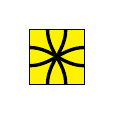
\begin{tikzpicture}[x=7mm,y=7mm]

\draw[black,fill=yellow] (0.000000,0.000000) rectangle (1.000000,-1.000000);
\draw[out=-90,in=90,looseness=1,very thick] (0.330000,0.000000) to (0.660000,-1.000000);
\draw[out=-90,in=90,looseness=1,very thick] (0.660000,0.000000) to (0.330000,-1.000000);
\draw[out=180,in=0,looseness=1,very thick] (1.000000,-0.330000) to (0.000000,-0.660000);
\draw[out=180,in=0,looseness=1,very thick] (1.000000,-0.660000) to (0.000000,-0.330000);
\end{tikzpicture}

\item Player 2 \textcolor{blue}{\LARGE$\bullet$} plays at row 3, col 5:
\begin{center}

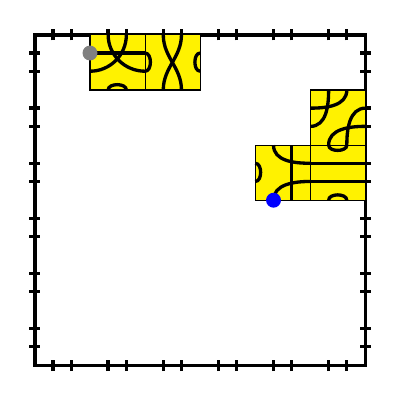
\begin{tikzpicture}[x=7mm,y=7mm]

\draw[very thick] (0.000000,0.000000) rectangle (6.000000,-6.000000);
\draw (0.000000,0.000000) grid[step=6] (6.000000,-6.000000);
\draw[very thick] (-0.100000,-0.330000) to (0.100000,-0.330000);
\draw[very thick] (5.900000,-0.330000) to (6.100000,-0.330000);
\draw[very thick] (0.330000,-0.100000) to (0.330000,0.100000);
\draw[very thick] (0.330000,-6.100000) to (0.330000,-5.900000);
\draw[very thick] (-0.100000,-0.660000) to (0.100000,-0.660000);
\draw[very thick] (5.900000,-0.660000) to (6.100000,-0.660000);
\draw[very thick] (0.660000,-0.100000) to (0.660000,0.100000);
\draw[very thick] (0.660000,-6.100000) to (0.660000,-5.900000);
\draw[very thick] (-0.100000,-1.330000) to (0.100000,-1.330000);
\draw[very thick] (5.900000,-1.330000) to (6.100000,-1.330000);
\draw[very thick] (1.330000,-0.100000) to (1.330000,0.100000);
\draw[very thick] (1.330000,-6.100000) to (1.330000,-5.900000);
\draw[very thick] (-0.100000,-1.660000) to (0.100000,-1.660000);
\draw[very thick] (5.900000,-1.660000) to (6.100000,-1.660000);
\draw[very thick] (1.660000,-0.100000) to (1.660000,0.100000);
\draw[very thick] (1.660000,-6.100000) to (1.660000,-5.900000);
\draw[very thick] (-0.100000,-2.330000) to (0.100000,-2.330000);
\draw[very thick] (5.900000,-2.330000) to (6.100000,-2.330000);
\draw[very thick] (2.330000,-0.100000) to (2.330000,0.100000);
\draw[very thick] (2.330000,-6.100000) to (2.330000,-5.900000);
\draw[very thick] (-0.100000,-2.660000) to (0.100000,-2.660000);
\draw[very thick] (5.900000,-2.660000) to (6.100000,-2.660000);
\draw[very thick] (2.660000,-0.100000) to (2.660000,0.100000);
\draw[very thick] (2.660000,-6.100000) to (2.660000,-5.900000);
\draw[very thick] (-0.100000,-3.330000) to (0.100000,-3.330000);
\draw[very thick] (5.900000,-3.330000) to (6.100000,-3.330000);
\draw[very thick] (3.330000,-0.100000) to (3.330000,0.100000);
\draw[very thick] (3.330000,-6.100000) to (3.330000,-5.900000);
\draw[very thick] (-0.100000,-3.660000) to (0.100000,-3.660000);
\draw[very thick] (5.900000,-3.660000) to (6.100000,-3.660000);
\draw[very thick] (3.660000,-0.100000) to (3.660000,0.100000);
\draw[very thick] (3.660000,-6.100000) to (3.660000,-5.900000);
\draw[very thick] (-0.100000,-4.330000) to (0.100000,-4.330000);
\draw[very thick] (5.900000,-4.330000) to (6.100000,-4.330000);
\draw[very thick] (4.330000,-0.100000) to (4.330000,0.100000);
\draw[very thick] (4.330000,-6.100000) to (4.330000,-5.900000);
\draw[very thick] (-0.100000,-4.660000) to (0.100000,-4.660000);
\draw[very thick] (5.900000,-4.660000) to (6.100000,-4.660000);
\draw[very thick] (4.660000,-0.100000) to (4.660000,0.100000);
\draw[very thick] (4.660000,-6.100000) to (4.660000,-5.900000);
\draw[very thick] (-0.100000,-5.330000) to (0.100000,-5.330000);
\draw[very thick] (5.900000,-5.330000) to (6.100000,-5.330000);
\draw[very thick] (5.330000,-0.100000) to (5.330000,0.100000);
\draw[very thick] (5.330000,-6.100000) to (5.330000,-5.900000);
\draw[very thick] (-0.100000,-5.660000) to (0.100000,-5.660000);
\draw[very thick] (5.900000,-5.660000) to (6.100000,-5.660000);
\draw[very thick] (5.660000,-0.100000) to (5.660000,0.100000);
\draw[very thick] (5.660000,-6.100000) to (5.660000,-5.900000);
\draw[black,fill=yellow] (1.000000,0.000000) rectangle (2.000000,-1.000000);
\draw[out=-90,in=180,looseness=1,very thick] (1.330000,0.000000) to (2.000000,-0.660000);
\draw[out=-90,in=0,looseness=1,very thick] (1.660000,0.000000) to (1.000000,-0.660000);
\draw[out=180,in=0,looseness=1,very thick] (2.000000,-0.330000) to (1.000000,-0.330000);
\draw[out=90,in=90,looseness=1,very thick] (1.660000,-1.000000) to (1.330000,-1.000000);
\draw[black,fill=yellow] (2.000000,0.000000) rectangle (3.000000,-1.000000);
\draw[out=-90,in=90,looseness=1,very thick] (2.330000,0.000000) to (2.660000,-1.000000);
\draw[out=-90,in=90,looseness=1,very thick] (2.660000,0.000000) to (2.330000,-1.000000);
\draw[out=180,in=180,looseness=1,very thick] (3.000000,-0.330000) to (3.000000,-0.660000);
\draw[out=0,in=0,looseness=1,very thick] (2.000000,-0.660000) to (2.000000,-0.330000);
\draw[black,fill=yellow] (4.000000,-2.000000) rectangle (5.000000,-3.000000);
\draw[out=-90,in=180,looseness=1,very thick] (4.330000,-2.000000) to (5.000000,-2.330000);
\draw[out=-90,in=90,looseness=1,very thick] (4.660000,-2.000000) to (4.660000,-3.000000);
\draw[out=180,in=90,looseness=1,very thick] (5.000000,-2.660000) to (4.330000,-3.000000);
\draw[out=0,in=0,looseness=1,very thick] (4.000000,-2.660000) to (4.000000,-2.330000);
\draw[black,fill=yellow] (5.000000,-1.000000) rectangle (6.000000,-2.000000);
\draw[out=-90,in=0,looseness=1,very thick] (5.330000,-1.000000) to (5.000000,-1.660000);
\draw[out=-90,in=0,looseness=1,very thick] (5.660000,-1.000000) to (5.000000,-1.330000);
\draw[out=180,in=90,looseness=1,very thick] (6.000000,-1.330000) to (5.660000,-2.000000);
\draw[out=180,in=90,looseness=1,very thick] (6.000000,-1.660000) to (5.330000,-2.000000);
\draw[black,fill=yellow] (5.000000,-2.000000) rectangle (6.000000,-3.000000);
\draw[out=-90,in=-90,looseness=1,very thick] (5.330000,-2.000000) to (5.660000,-2.000000);
\draw[out=180,in=0,looseness=1,very thick] (6.000000,-2.330000) to (5.000000,-2.330000);
\draw[out=180,in=0,looseness=1,very thick] (6.000000,-2.660000) to (5.000000,-2.660000);
\draw[out=90,in=90,looseness=1,very thick] (5.660000,-3.000000) to (5.330000,-3.000000);
\draw[draw=blue,fill=blue] (4.330000,-3.000000) circle [x radius=0.125000,y radius=0.125000];
\draw[draw=gray,fill=gray] (1.000000,-0.330000) circle [x radius=0.125000,y radius=0.125000];
\end{tikzpicture}

\end{center}

\item[(17)] Player 2 \textcolor{blue}{\LARGE$\bullet$} draws 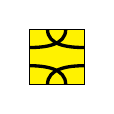
\begin{tikzpicture}[x=7mm,y=7mm]

\draw[black,fill=yellow] (0.000000,0.000000) rectangle (1.000000,-1.000000);
\draw[out=-90,in=180,looseness=1,very thick] (0.330000,0.000000) to (1.000000,-0.330000);
\draw[out=-90,in=0,looseness=1,very thick] (0.660000,0.000000) to (0.000000,-0.330000);
\draw[out=180,in=90,looseness=1,very thick] (1.000000,-0.660000) to (0.330000,-1.000000);
\draw[out=90,in=0,looseness=1,very thick] (0.660000,-1.000000) to (0.000000,-0.660000);
\end{tikzpicture}

\item Player 1 \textcolor{gray}{\LARGE$\bullet$} plays at row 1, col 1:
\begin{center}

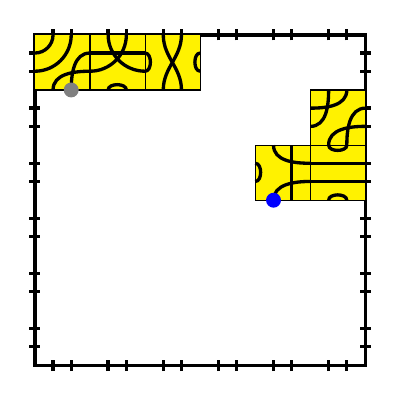
\begin{tikzpicture}[x=7mm,y=7mm]

\draw[very thick] (0.000000,0.000000) rectangle (6.000000,-6.000000);
\draw (0.000000,0.000000) grid[step=6] (6.000000,-6.000000);
\draw[very thick] (-0.100000,-0.330000) to (0.100000,-0.330000);
\draw[very thick] (5.900000,-0.330000) to (6.100000,-0.330000);
\draw[very thick] (0.330000,-0.100000) to (0.330000,0.100000);
\draw[very thick] (0.330000,-6.100000) to (0.330000,-5.900000);
\draw[very thick] (-0.100000,-0.660000) to (0.100000,-0.660000);
\draw[very thick] (5.900000,-0.660000) to (6.100000,-0.660000);
\draw[very thick] (0.660000,-0.100000) to (0.660000,0.100000);
\draw[very thick] (0.660000,-6.100000) to (0.660000,-5.900000);
\draw[very thick] (-0.100000,-1.330000) to (0.100000,-1.330000);
\draw[very thick] (5.900000,-1.330000) to (6.100000,-1.330000);
\draw[very thick] (1.330000,-0.100000) to (1.330000,0.100000);
\draw[very thick] (1.330000,-6.100000) to (1.330000,-5.900000);
\draw[very thick] (-0.100000,-1.660000) to (0.100000,-1.660000);
\draw[very thick] (5.900000,-1.660000) to (6.100000,-1.660000);
\draw[very thick] (1.660000,-0.100000) to (1.660000,0.100000);
\draw[very thick] (1.660000,-6.100000) to (1.660000,-5.900000);
\draw[very thick] (-0.100000,-2.330000) to (0.100000,-2.330000);
\draw[very thick] (5.900000,-2.330000) to (6.100000,-2.330000);
\draw[very thick] (2.330000,-0.100000) to (2.330000,0.100000);
\draw[very thick] (2.330000,-6.100000) to (2.330000,-5.900000);
\draw[very thick] (-0.100000,-2.660000) to (0.100000,-2.660000);
\draw[very thick] (5.900000,-2.660000) to (6.100000,-2.660000);
\draw[very thick] (2.660000,-0.100000) to (2.660000,0.100000);
\draw[very thick] (2.660000,-6.100000) to (2.660000,-5.900000);
\draw[very thick] (-0.100000,-3.330000) to (0.100000,-3.330000);
\draw[very thick] (5.900000,-3.330000) to (6.100000,-3.330000);
\draw[very thick] (3.330000,-0.100000) to (3.330000,0.100000);
\draw[very thick] (3.330000,-6.100000) to (3.330000,-5.900000);
\draw[very thick] (-0.100000,-3.660000) to (0.100000,-3.660000);
\draw[very thick] (5.900000,-3.660000) to (6.100000,-3.660000);
\draw[very thick] (3.660000,-0.100000) to (3.660000,0.100000);
\draw[very thick] (3.660000,-6.100000) to (3.660000,-5.900000);
\draw[very thick] (-0.100000,-4.330000) to (0.100000,-4.330000);
\draw[very thick] (5.900000,-4.330000) to (6.100000,-4.330000);
\draw[very thick] (4.330000,-0.100000) to (4.330000,0.100000);
\draw[very thick] (4.330000,-6.100000) to (4.330000,-5.900000);
\draw[very thick] (-0.100000,-4.660000) to (0.100000,-4.660000);
\draw[very thick] (5.900000,-4.660000) to (6.100000,-4.660000);
\draw[very thick] (4.660000,-0.100000) to (4.660000,0.100000);
\draw[very thick] (4.660000,-6.100000) to (4.660000,-5.900000);
\draw[very thick] (-0.100000,-5.330000) to (0.100000,-5.330000);
\draw[very thick] (5.900000,-5.330000) to (6.100000,-5.330000);
\draw[very thick] (5.330000,-0.100000) to (5.330000,0.100000);
\draw[very thick] (5.330000,-6.100000) to (5.330000,-5.900000);
\draw[very thick] (-0.100000,-5.660000) to (0.100000,-5.660000);
\draw[very thick] (5.900000,-5.660000) to (6.100000,-5.660000);
\draw[very thick] (5.660000,-0.100000) to (5.660000,0.100000);
\draw[very thick] (5.660000,-6.100000) to (5.660000,-5.900000);
\draw[black,fill=yellow] (0.000000,0.000000) rectangle (1.000000,-1.000000);
\draw[out=-90,in=0,looseness=1,very thick] (0.330000,0.000000) to (0.000000,-0.330000);
\draw[out=-90,in=0,looseness=1,very thick] (0.660000,0.000000) to (0.000000,-0.660000);
\draw[out=180,in=90,looseness=1,very thick] (1.000000,-0.330000) to (0.660000,-1.000000);
\draw[out=180,in=90,looseness=1,very thick] (1.000000,-0.660000) to (0.330000,-1.000000);
\draw[black,fill=yellow] (1.000000,0.000000) rectangle (2.000000,-1.000000);
\draw[out=-90,in=180,looseness=1,very thick] (1.330000,0.000000) to (2.000000,-0.660000);
\draw[out=-90,in=0,looseness=1,very thick] (1.660000,0.000000) to (1.000000,-0.660000);
\draw[out=180,in=0,looseness=1,very thick] (2.000000,-0.330000) to (1.000000,-0.330000);
\draw[out=90,in=90,looseness=1,very thick] (1.660000,-1.000000) to (1.330000,-1.000000);
\draw[black,fill=yellow] (2.000000,0.000000) rectangle (3.000000,-1.000000);
\draw[out=-90,in=90,looseness=1,very thick] (2.330000,0.000000) to (2.660000,-1.000000);
\draw[out=-90,in=90,looseness=1,very thick] (2.660000,0.000000) to (2.330000,-1.000000);
\draw[out=180,in=180,looseness=1,very thick] (3.000000,-0.330000) to (3.000000,-0.660000);
\draw[out=0,in=0,looseness=1,very thick] (2.000000,-0.660000) to (2.000000,-0.330000);
\draw[black,fill=yellow] (4.000000,-2.000000) rectangle (5.000000,-3.000000);
\draw[out=-90,in=180,looseness=1,very thick] (4.330000,-2.000000) to (5.000000,-2.330000);
\draw[out=-90,in=90,looseness=1,very thick] (4.660000,-2.000000) to (4.660000,-3.000000);
\draw[out=180,in=90,looseness=1,very thick] (5.000000,-2.660000) to (4.330000,-3.000000);
\draw[out=0,in=0,looseness=1,very thick] (4.000000,-2.660000) to (4.000000,-2.330000);
\draw[black,fill=yellow] (5.000000,-1.000000) rectangle (6.000000,-2.000000);
\draw[out=-90,in=0,looseness=1,very thick] (5.330000,-1.000000) to (5.000000,-1.660000);
\draw[out=-90,in=0,looseness=1,very thick] (5.660000,-1.000000) to (5.000000,-1.330000);
\draw[out=180,in=90,looseness=1,very thick] (6.000000,-1.330000) to (5.660000,-2.000000);
\draw[out=180,in=90,looseness=1,very thick] (6.000000,-1.660000) to (5.330000,-2.000000);
\draw[black,fill=yellow] (5.000000,-2.000000) rectangle (6.000000,-3.000000);
\draw[out=-90,in=-90,looseness=1,very thick] (5.330000,-2.000000) to (5.660000,-2.000000);
\draw[out=180,in=0,looseness=1,very thick] (6.000000,-2.330000) to (5.000000,-2.330000);
\draw[out=180,in=0,looseness=1,very thick] (6.000000,-2.660000) to (5.000000,-2.660000);
\draw[out=90,in=90,looseness=1,very thick] (5.660000,-3.000000) to (5.330000,-3.000000);
\draw[draw=blue,fill=blue] (4.330000,-3.000000) circle [x radius=0.125000,y radius=0.125000];
\draw[draw=gray,fill=gray] (0.660000,-1.000000) circle [x radius=0.125000,y radius=0.125000];
\end{tikzpicture}

\end{center}

\item[(18)] Player 1 \textcolor{gray}{\LARGE$\bullet$} draws 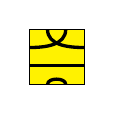
\begin{tikzpicture}[x=7mm,y=7mm]

\draw[black,fill=yellow] (0.000000,0.000000) rectangle (1.000000,-1.000000);
\draw[out=-90,in=180,looseness=1,very thick] (0.330000,0.000000) to (1.000000,-0.330000);
\draw[out=-90,in=0,looseness=1,very thick] (0.660000,0.000000) to (0.000000,-0.330000);
\draw[out=180,in=0,looseness=1,very thick] (1.000000,-0.660000) to (0.000000,-0.660000);
\draw[out=90,in=90,looseness=1,very thick] (0.660000,-1.000000) to (0.330000,-1.000000);
\end{tikzpicture}

\item Player 2 \textcolor{blue}{\LARGE$\bullet$} plays at row 4, col 5:
\begin{center}

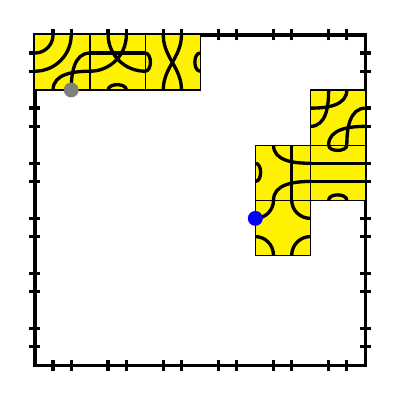
\begin{tikzpicture}[x=7mm,y=7mm]

\draw[very thick] (0.000000,0.000000) rectangle (6.000000,-6.000000);
\draw (0.000000,0.000000) grid[step=6] (6.000000,-6.000000);
\draw[very thick] (-0.100000,-0.330000) to (0.100000,-0.330000);
\draw[very thick] (5.900000,-0.330000) to (6.100000,-0.330000);
\draw[very thick] (0.330000,-0.100000) to (0.330000,0.100000);
\draw[very thick] (0.330000,-6.100000) to (0.330000,-5.900000);
\draw[very thick] (-0.100000,-0.660000) to (0.100000,-0.660000);
\draw[very thick] (5.900000,-0.660000) to (6.100000,-0.660000);
\draw[very thick] (0.660000,-0.100000) to (0.660000,0.100000);
\draw[very thick] (0.660000,-6.100000) to (0.660000,-5.900000);
\draw[very thick] (-0.100000,-1.330000) to (0.100000,-1.330000);
\draw[very thick] (5.900000,-1.330000) to (6.100000,-1.330000);
\draw[very thick] (1.330000,-0.100000) to (1.330000,0.100000);
\draw[very thick] (1.330000,-6.100000) to (1.330000,-5.900000);
\draw[very thick] (-0.100000,-1.660000) to (0.100000,-1.660000);
\draw[very thick] (5.900000,-1.660000) to (6.100000,-1.660000);
\draw[very thick] (1.660000,-0.100000) to (1.660000,0.100000);
\draw[very thick] (1.660000,-6.100000) to (1.660000,-5.900000);
\draw[very thick] (-0.100000,-2.330000) to (0.100000,-2.330000);
\draw[very thick] (5.900000,-2.330000) to (6.100000,-2.330000);
\draw[very thick] (2.330000,-0.100000) to (2.330000,0.100000);
\draw[very thick] (2.330000,-6.100000) to (2.330000,-5.900000);
\draw[very thick] (-0.100000,-2.660000) to (0.100000,-2.660000);
\draw[very thick] (5.900000,-2.660000) to (6.100000,-2.660000);
\draw[very thick] (2.660000,-0.100000) to (2.660000,0.100000);
\draw[very thick] (2.660000,-6.100000) to (2.660000,-5.900000);
\draw[very thick] (-0.100000,-3.330000) to (0.100000,-3.330000);
\draw[very thick] (5.900000,-3.330000) to (6.100000,-3.330000);
\draw[very thick] (3.330000,-0.100000) to (3.330000,0.100000);
\draw[very thick] (3.330000,-6.100000) to (3.330000,-5.900000);
\draw[very thick] (-0.100000,-3.660000) to (0.100000,-3.660000);
\draw[very thick] (5.900000,-3.660000) to (6.100000,-3.660000);
\draw[very thick] (3.660000,-0.100000) to (3.660000,0.100000);
\draw[very thick] (3.660000,-6.100000) to (3.660000,-5.900000);
\draw[very thick] (-0.100000,-4.330000) to (0.100000,-4.330000);
\draw[very thick] (5.900000,-4.330000) to (6.100000,-4.330000);
\draw[very thick] (4.330000,-0.100000) to (4.330000,0.100000);
\draw[very thick] (4.330000,-6.100000) to (4.330000,-5.900000);
\draw[very thick] (-0.100000,-4.660000) to (0.100000,-4.660000);
\draw[very thick] (5.900000,-4.660000) to (6.100000,-4.660000);
\draw[very thick] (4.660000,-0.100000) to (4.660000,0.100000);
\draw[very thick] (4.660000,-6.100000) to (4.660000,-5.900000);
\draw[very thick] (-0.100000,-5.330000) to (0.100000,-5.330000);
\draw[very thick] (5.900000,-5.330000) to (6.100000,-5.330000);
\draw[very thick] (5.330000,-0.100000) to (5.330000,0.100000);
\draw[very thick] (5.330000,-6.100000) to (5.330000,-5.900000);
\draw[very thick] (-0.100000,-5.660000) to (0.100000,-5.660000);
\draw[very thick] (5.900000,-5.660000) to (6.100000,-5.660000);
\draw[very thick] (5.660000,-0.100000) to (5.660000,0.100000);
\draw[very thick] (5.660000,-6.100000) to (5.660000,-5.900000);
\draw[black,fill=yellow] (0.000000,0.000000) rectangle (1.000000,-1.000000);
\draw[out=-90,in=0,looseness=1,very thick] (0.330000,0.000000) to (0.000000,-0.330000);
\draw[out=-90,in=0,looseness=1,very thick] (0.660000,0.000000) to (0.000000,-0.660000);
\draw[out=180,in=90,looseness=1,very thick] (1.000000,-0.330000) to (0.660000,-1.000000);
\draw[out=180,in=90,looseness=1,very thick] (1.000000,-0.660000) to (0.330000,-1.000000);
\draw[black,fill=yellow] (1.000000,0.000000) rectangle (2.000000,-1.000000);
\draw[out=-90,in=180,looseness=1,very thick] (1.330000,0.000000) to (2.000000,-0.660000);
\draw[out=-90,in=0,looseness=1,very thick] (1.660000,0.000000) to (1.000000,-0.660000);
\draw[out=180,in=0,looseness=1,very thick] (2.000000,-0.330000) to (1.000000,-0.330000);
\draw[out=90,in=90,looseness=1,very thick] (1.660000,-1.000000) to (1.330000,-1.000000);
\draw[black,fill=yellow] (2.000000,0.000000) rectangle (3.000000,-1.000000);
\draw[out=-90,in=90,looseness=1,very thick] (2.330000,0.000000) to (2.660000,-1.000000);
\draw[out=-90,in=90,looseness=1,very thick] (2.660000,0.000000) to (2.330000,-1.000000);
\draw[out=180,in=180,looseness=1,very thick] (3.000000,-0.330000) to (3.000000,-0.660000);
\draw[out=0,in=0,looseness=1,very thick] (2.000000,-0.660000) to (2.000000,-0.330000);
\draw[black,fill=yellow] (4.000000,-2.000000) rectangle (5.000000,-3.000000);
\draw[out=-90,in=180,looseness=1,very thick] (4.330000,-2.000000) to (5.000000,-2.330000);
\draw[out=-90,in=90,looseness=1,very thick] (4.660000,-2.000000) to (4.660000,-3.000000);
\draw[out=180,in=90,looseness=1,very thick] (5.000000,-2.660000) to (4.330000,-3.000000);
\draw[out=0,in=0,looseness=1,very thick] (4.000000,-2.660000) to (4.000000,-2.330000);
\draw[black,fill=yellow] (4.000000,-3.000000) rectangle (5.000000,-4.000000);
\draw[out=-90,in=0,looseness=1,very thick] (4.330000,-3.000000) to (4.000000,-3.330000);
\draw[out=-90,in=180,looseness=1,very thick] (4.660000,-3.000000) to (5.000000,-3.330000);
\draw[out=180,in=90,looseness=1,very thick] (5.000000,-3.660000) to (4.660000,-4.000000);
\draw[out=90,in=0,looseness=1,very thick] (4.330000,-4.000000) to (4.000000,-3.660000);
\draw[black,fill=yellow] (5.000000,-1.000000) rectangle (6.000000,-2.000000);
\draw[out=-90,in=0,looseness=1,very thick] (5.330000,-1.000000) to (5.000000,-1.660000);
\draw[out=-90,in=0,looseness=1,very thick] (5.660000,-1.000000) to (5.000000,-1.330000);
\draw[out=180,in=90,looseness=1,very thick] (6.000000,-1.330000) to (5.660000,-2.000000);
\draw[out=180,in=90,looseness=1,very thick] (6.000000,-1.660000) to (5.330000,-2.000000);
\draw[black,fill=yellow] (5.000000,-2.000000) rectangle (6.000000,-3.000000);
\draw[out=-90,in=-90,looseness=1,very thick] (5.330000,-2.000000) to (5.660000,-2.000000);
\draw[out=180,in=0,looseness=1,very thick] (6.000000,-2.330000) to (5.000000,-2.330000);
\draw[out=180,in=0,looseness=1,very thick] (6.000000,-2.660000) to (5.000000,-2.660000);
\draw[out=90,in=90,looseness=1,very thick] (5.660000,-3.000000) to (5.330000,-3.000000);
\draw[draw=blue,fill=blue] (4.000000,-3.330000) circle [x radius=0.125000,y radius=0.125000];
\draw[draw=gray,fill=gray] (0.660000,-1.000000) circle [x radius=0.125000,y radius=0.125000];
\end{tikzpicture}

\end{center}

\item[(19)] Player 2 \textcolor{blue}{\LARGE$\bullet$} draws 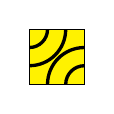
\begin{tikzpicture}[x=7mm,y=7mm]

\draw[black,fill=yellow] (0.000000,0.000000) rectangle (1.000000,-1.000000);
\draw[out=-90,in=0,looseness=1,very thick] (0.330000,0.000000) to (0.000000,-0.330000);
\draw[out=-90,in=0,looseness=1,very thick] (0.660000,0.000000) to (0.000000,-0.660000);
\draw[out=180,in=90,looseness=1,very thick] (1.000000,-0.330000) to (0.330000,-1.000000);
\draw[out=180,in=90,looseness=1,very thick] (1.000000,-0.660000) to (0.660000,-1.000000);
\end{tikzpicture}

\item Player 1 \textcolor{gray}{\LARGE$\bullet$} plays at row 2, col 1:
\begin{center}

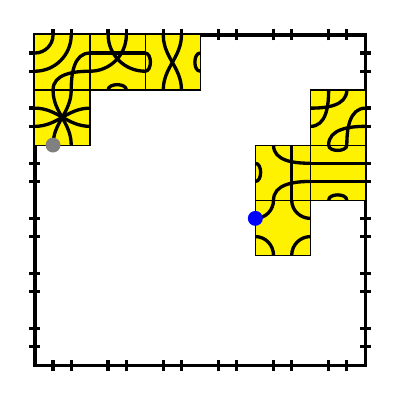
\begin{tikzpicture}[x=7mm,y=7mm]

\draw[very thick] (0.000000,0.000000) rectangle (6.000000,-6.000000);
\draw (0.000000,0.000000) grid[step=6] (6.000000,-6.000000);
\draw[very thick] (-0.100000,-0.330000) to (0.100000,-0.330000);
\draw[very thick] (5.900000,-0.330000) to (6.100000,-0.330000);
\draw[very thick] (0.330000,-0.100000) to (0.330000,0.100000);
\draw[very thick] (0.330000,-6.100000) to (0.330000,-5.900000);
\draw[very thick] (-0.100000,-0.660000) to (0.100000,-0.660000);
\draw[very thick] (5.900000,-0.660000) to (6.100000,-0.660000);
\draw[very thick] (0.660000,-0.100000) to (0.660000,0.100000);
\draw[very thick] (0.660000,-6.100000) to (0.660000,-5.900000);
\draw[very thick] (-0.100000,-1.330000) to (0.100000,-1.330000);
\draw[very thick] (5.900000,-1.330000) to (6.100000,-1.330000);
\draw[very thick] (1.330000,-0.100000) to (1.330000,0.100000);
\draw[very thick] (1.330000,-6.100000) to (1.330000,-5.900000);
\draw[very thick] (-0.100000,-1.660000) to (0.100000,-1.660000);
\draw[very thick] (5.900000,-1.660000) to (6.100000,-1.660000);
\draw[very thick] (1.660000,-0.100000) to (1.660000,0.100000);
\draw[very thick] (1.660000,-6.100000) to (1.660000,-5.900000);
\draw[very thick] (-0.100000,-2.330000) to (0.100000,-2.330000);
\draw[very thick] (5.900000,-2.330000) to (6.100000,-2.330000);
\draw[very thick] (2.330000,-0.100000) to (2.330000,0.100000);
\draw[very thick] (2.330000,-6.100000) to (2.330000,-5.900000);
\draw[very thick] (-0.100000,-2.660000) to (0.100000,-2.660000);
\draw[very thick] (5.900000,-2.660000) to (6.100000,-2.660000);
\draw[very thick] (2.660000,-0.100000) to (2.660000,0.100000);
\draw[very thick] (2.660000,-6.100000) to (2.660000,-5.900000);
\draw[very thick] (-0.100000,-3.330000) to (0.100000,-3.330000);
\draw[very thick] (5.900000,-3.330000) to (6.100000,-3.330000);
\draw[very thick] (3.330000,-0.100000) to (3.330000,0.100000);
\draw[very thick] (3.330000,-6.100000) to (3.330000,-5.900000);
\draw[very thick] (-0.100000,-3.660000) to (0.100000,-3.660000);
\draw[very thick] (5.900000,-3.660000) to (6.100000,-3.660000);
\draw[very thick] (3.660000,-0.100000) to (3.660000,0.100000);
\draw[very thick] (3.660000,-6.100000) to (3.660000,-5.900000);
\draw[very thick] (-0.100000,-4.330000) to (0.100000,-4.330000);
\draw[very thick] (5.900000,-4.330000) to (6.100000,-4.330000);
\draw[very thick] (4.330000,-0.100000) to (4.330000,0.100000);
\draw[very thick] (4.330000,-6.100000) to (4.330000,-5.900000);
\draw[very thick] (-0.100000,-4.660000) to (0.100000,-4.660000);
\draw[very thick] (5.900000,-4.660000) to (6.100000,-4.660000);
\draw[very thick] (4.660000,-0.100000) to (4.660000,0.100000);
\draw[very thick] (4.660000,-6.100000) to (4.660000,-5.900000);
\draw[very thick] (-0.100000,-5.330000) to (0.100000,-5.330000);
\draw[very thick] (5.900000,-5.330000) to (6.100000,-5.330000);
\draw[very thick] (5.330000,-0.100000) to (5.330000,0.100000);
\draw[very thick] (5.330000,-6.100000) to (5.330000,-5.900000);
\draw[very thick] (-0.100000,-5.660000) to (0.100000,-5.660000);
\draw[very thick] (5.900000,-5.660000) to (6.100000,-5.660000);
\draw[very thick] (5.660000,-0.100000) to (5.660000,0.100000);
\draw[very thick] (5.660000,-6.100000) to (5.660000,-5.900000);
\draw[black,fill=yellow] (0.000000,0.000000) rectangle (1.000000,-1.000000);
\draw[out=-90,in=0,looseness=1,very thick] (0.330000,0.000000) to (0.000000,-0.330000);
\draw[out=-90,in=0,looseness=1,very thick] (0.660000,0.000000) to (0.000000,-0.660000);
\draw[out=180,in=90,looseness=1,very thick] (1.000000,-0.330000) to (0.660000,-1.000000);
\draw[out=180,in=90,looseness=1,very thick] (1.000000,-0.660000) to (0.330000,-1.000000);
\draw[black,fill=yellow] (0.000000,-1.000000) rectangle (1.000000,-2.000000);
\draw[out=-90,in=90,looseness=1,very thick] (0.330000,-1.000000) to (0.660000,-2.000000);
\draw[out=-90,in=90,looseness=1,very thick] (0.660000,-1.000000) to (0.330000,-2.000000);
\draw[out=180,in=0,looseness=1,very thick] (1.000000,-1.330000) to (0.000000,-1.660000);
\draw[out=180,in=0,looseness=1,very thick] (1.000000,-1.660000) to (0.000000,-1.330000);
\draw[black,fill=yellow] (1.000000,0.000000) rectangle (2.000000,-1.000000);
\draw[out=-90,in=180,looseness=1,very thick] (1.330000,0.000000) to (2.000000,-0.660000);
\draw[out=-90,in=0,looseness=1,very thick] (1.660000,0.000000) to (1.000000,-0.660000);
\draw[out=180,in=0,looseness=1,very thick] (2.000000,-0.330000) to (1.000000,-0.330000);
\draw[out=90,in=90,looseness=1,very thick] (1.660000,-1.000000) to (1.330000,-1.000000);
\draw[black,fill=yellow] (2.000000,0.000000) rectangle (3.000000,-1.000000);
\draw[out=-90,in=90,looseness=1,very thick] (2.330000,0.000000) to (2.660000,-1.000000);
\draw[out=-90,in=90,looseness=1,very thick] (2.660000,0.000000) to (2.330000,-1.000000);
\draw[out=180,in=180,looseness=1,very thick] (3.000000,-0.330000) to (3.000000,-0.660000);
\draw[out=0,in=0,looseness=1,very thick] (2.000000,-0.660000) to (2.000000,-0.330000);
\draw[black,fill=yellow] (4.000000,-2.000000) rectangle (5.000000,-3.000000);
\draw[out=-90,in=180,looseness=1,very thick] (4.330000,-2.000000) to (5.000000,-2.330000);
\draw[out=-90,in=90,looseness=1,very thick] (4.660000,-2.000000) to (4.660000,-3.000000);
\draw[out=180,in=90,looseness=1,very thick] (5.000000,-2.660000) to (4.330000,-3.000000);
\draw[out=0,in=0,looseness=1,very thick] (4.000000,-2.660000) to (4.000000,-2.330000);
\draw[black,fill=yellow] (4.000000,-3.000000) rectangle (5.000000,-4.000000);
\draw[out=-90,in=0,looseness=1,very thick] (4.330000,-3.000000) to (4.000000,-3.330000);
\draw[out=-90,in=180,looseness=1,very thick] (4.660000,-3.000000) to (5.000000,-3.330000);
\draw[out=180,in=90,looseness=1,very thick] (5.000000,-3.660000) to (4.660000,-4.000000);
\draw[out=90,in=0,looseness=1,very thick] (4.330000,-4.000000) to (4.000000,-3.660000);
\draw[black,fill=yellow] (5.000000,-1.000000) rectangle (6.000000,-2.000000);
\draw[out=-90,in=0,looseness=1,very thick] (5.330000,-1.000000) to (5.000000,-1.660000);
\draw[out=-90,in=0,looseness=1,very thick] (5.660000,-1.000000) to (5.000000,-1.330000);
\draw[out=180,in=90,looseness=1,very thick] (6.000000,-1.330000) to (5.660000,-2.000000);
\draw[out=180,in=90,looseness=1,very thick] (6.000000,-1.660000) to (5.330000,-2.000000);
\draw[black,fill=yellow] (5.000000,-2.000000) rectangle (6.000000,-3.000000);
\draw[out=-90,in=-90,looseness=1,very thick] (5.330000,-2.000000) to (5.660000,-2.000000);
\draw[out=180,in=0,looseness=1,very thick] (6.000000,-2.330000) to (5.000000,-2.330000);
\draw[out=180,in=0,looseness=1,very thick] (6.000000,-2.660000) to (5.000000,-2.660000);
\draw[out=90,in=90,looseness=1,very thick] (5.660000,-3.000000) to (5.330000,-3.000000);
\draw[draw=blue,fill=blue] (4.000000,-3.330000) circle [x radius=0.125000,y radius=0.125000];
\draw[draw=gray,fill=gray] (0.330000,-2.000000) circle [x radius=0.125000,y radius=0.125000];
\end{tikzpicture}

\end{center}

\item[(20)] Player 1 \textcolor{gray}{\LARGE$\bullet$} draws 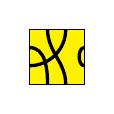
\begin{tikzpicture}[x=7mm,y=7mm]

\draw[black,fill=yellow] (0.000000,0.000000) rectangle (1.000000,-1.000000);
\draw[out=-90,in=90,looseness=1,very thick] (0.330000,0.000000) to (0.660000,-1.000000);
\draw[out=-90,in=0,looseness=1,very thick] (0.660000,0.000000) to (0.000000,-0.660000);
\draw[out=180,in=180,looseness=1,very thick] (1.000000,-0.330000) to (1.000000,-0.660000);
\draw[out=90,in=0,looseness=1,very thick] (0.330000,-1.000000) to (0.000000,-0.330000);
\end{tikzpicture}

\item Player 2 \textcolor{blue}{\LARGE$\bullet$} plays at row 4, col 4:
\begin{center}

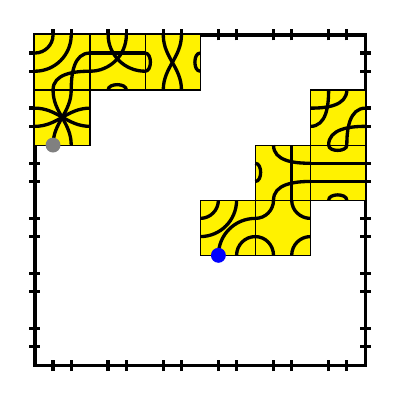
\begin{tikzpicture}[x=7mm,y=7mm]

\draw[very thick] (0.000000,0.000000) rectangle (6.000000,-6.000000);
\draw (0.000000,0.000000) grid[step=6] (6.000000,-6.000000);
\draw[very thick] (-0.100000,-0.330000) to (0.100000,-0.330000);
\draw[very thick] (5.900000,-0.330000) to (6.100000,-0.330000);
\draw[very thick] (0.330000,-0.100000) to (0.330000,0.100000);
\draw[very thick] (0.330000,-6.100000) to (0.330000,-5.900000);
\draw[very thick] (-0.100000,-0.660000) to (0.100000,-0.660000);
\draw[very thick] (5.900000,-0.660000) to (6.100000,-0.660000);
\draw[very thick] (0.660000,-0.100000) to (0.660000,0.100000);
\draw[very thick] (0.660000,-6.100000) to (0.660000,-5.900000);
\draw[very thick] (-0.100000,-1.330000) to (0.100000,-1.330000);
\draw[very thick] (5.900000,-1.330000) to (6.100000,-1.330000);
\draw[very thick] (1.330000,-0.100000) to (1.330000,0.100000);
\draw[very thick] (1.330000,-6.100000) to (1.330000,-5.900000);
\draw[very thick] (-0.100000,-1.660000) to (0.100000,-1.660000);
\draw[very thick] (5.900000,-1.660000) to (6.100000,-1.660000);
\draw[very thick] (1.660000,-0.100000) to (1.660000,0.100000);
\draw[very thick] (1.660000,-6.100000) to (1.660000,-5.900000);
\draw[very thick] (-0.100000,-2.330000) to (0.100000,-2.330000);
\draw[very thick] (5.900000,-2.330000) to (6.100000,-2.330000);
\draw[very thick] (2.330000,-0.100000) to (2.330000,0.100000);
\draw[very thick] (2.330000,-6.100000) to (2.330000,-5.900000);
\draw[very thick] (-0.100000,-2.660000) to (0.100000,-2.660000);
\draw[very thick] (5.900000,-2.660000) to (6.100000,-2.660000);
\draw[very thick] (2.660000,-0.100000) to (2.660000,0.100000);
\draw[very thick] (2.660000,-6.100000) to (2.660000,-5.900000);
\draw[very thick] (-0.100000,-3.330000) to (0.100000,-3.330000);
\draw[very thick] (5.900000,-3.330000) to (6.100000,-3.330000);
\draw[very thick] (3.330000,-0.100000) to (3.330000,0.100000);
\draw[very thick] (3.330000,-6.100000) to (3.330000,-5.900000);
\draw[very thick] (-0.100000,-3.660000) to (0.100000,-3.660000);
\draw[very thick] (5.900000,-3.660000) to (6.100000,-3.660000);
\draw[very thick] (3.660000,-0.100000) to (3.660000,0.100000);
\draw[very thick] (3.660000,-6.100000) to (3.660000,-5.900000);
\draw[very thick] (-0.100000,-4.330000) to (0.100000,-4.330000);
\draw[very thick] (5.900000,-4.330000) to (6.100000,-4.330000);
\draw[very thick] (4.330000,-0.100000) to (4.330000,0.100000);
\draw[very thick] (4.330000,-6.100000) to (4.330000,-5.900000);
\draw[very thick] (-0.100000,-4.660000) to (0.100000,-4.660000);
\draw[very thick] (5.900000,-4.660000) to (6.100000,-4.660000);
\draw[very thick] (4.660000,-0.100000) to (4.660000,0.100000);
\draw[very thick] (4.660000,-6.100000) to (4.660000,-5.900000);
\draw[very thick] (-0.100000,-5.330000) to (0.100000,-5.330000);
\draw[very thick] (5.900000,-5.330000) to (6.100000,-5.330000);
\draw[very thick] (5.330000,-0.100000) to (5.330000,0.100000);
\draw[very thick] (5.330000,-6.100000) to (5.330000,-5.900000);
\draw[very thick] (-0.100000,-5.660000) to (0.100000,-5.660000);
\draw[very thick] (5.900000,-5.660000) to (6.100000,-5.660000);
\draw[very thick] (5.660000,-0.100000) to (5.660000,0.100000);
\draw[very thick] (5.660000,-6.100000) to (5.660000,-5.900000);
\draw[black,fill=yellow] (0.000000,0.000000) rectangle (1.000000,-1.000000);
\draw[out=-90,in=0,looseness=1,very thick] (0.330000,0.000000) to (0.000000,-0.330000);
\draw[out=-90,in=0,looseness=1,very thick] (0.660000,0.000000) to (0.000000,-0.660000);
\draw[out=180,in=90,looseness=1,very thick] (1.000000,-0.330000) to (0.660000,-1.000000);
\draw[out=180,in=90,looseness=1,very thick] (1.000000,-0.660000) to (0.330000,-1.000000);
\draw[black,fill=yellow] (0.000000,-1.000000) rectangle (1.000000,-2.000000);
\draw[out=-90,in=90,looseness=1,very thick] (0.330000,-1.000000) to (0.660000,-2.000000);
\draw[out=-90,in=90,looseness=1,very thick] (0.660000,-1.000000) to (0.330000,-2.000000);
\draw[out=180,in=0,looseness=1,very thick] (1.000000,-1.330000) to (0.000000,-1.660000);
\draw[out=180,in=0,looseness=1,very thick] (1.000000,-1.660000) to (0.000000,-1.330000);
\draw[black,fill=yellow] (1.000000,0.000000) rectangle (2.000000,-1.000000);
\draw[out=-90,in=180,looseness=1,very thick] (1.330000,0.000000) to (2.000000,-0.660000);
\draw[out=-90,in=0,looseness=1,very thick] (1.660000,0.000000) to (1.000000,-0.660000);
\draw[out=180,in=0,looseness=1,very thick] (2.000000,-0.330000) to (1.000000,-0.330000);
\draw[out=90,in=90,looseness=1,very thick] (1.660000,-1.000000) to (1.330000,-1.000000);
\draw[black,fill=yellow] (2.000000,0.000000) rectangle (3.000000,-1.000000);
\draw[out=-90,in=90,looseness=1,very thick] (2.330000,0.000000) to (2.660000,-1.000000);
\draw[out=-90,in=90,looseness=1,very thick] (2.660000,0.000000) to (2.330000,-1.000000);
\draw[out=180,in=180,looseness=1,very thick] (3.000000,-0.330000) to (3.000000,-0.660000);
\draw[out=0,in=0,looseness=1,very thick] (2.000000,-0.660000) to (2.000000,-0.330000);
\draw[black,fill=yellow] (3.000000,-3.000000) rectangle (4.000000,-4.000000);
\draw[out=-90,in=0,looseness=1,very thick] (3.330000,-3.000000) to (3.000000,-3.330000);
\draw[out=-90,in=0,looseness=1,very thick] (3.660000,-3.000000) to (3.000000,-3.660000);
\draw[out=180,in=90,looseness=1,very thick] (4.000000,-3.330000) to (3.330000,-4.000000);
\draw[out=180,in=90,looseness=1,very thick] (4.000000,-3.660000) to (3.660000,-4.000000);
\draw[black,fill=yellow] (4.000000,-2.000000) rectangle (5.000000,-3.000000);
\draw[out=-90,in=180,looseness=1,very thick] (4.330000,-2.000000) to (5.000000,-2.330000);
\draw[out=-90,in=90,looseness=1,very thick] (4.660000,-2.000000) to (4.660000,-3.000000);
\draw[out=180,in=90,looseness=1,very thick] (5.000000,-2.660000) to (4.330000,-3.000000);
\draw[out=0,in=0,looseness=1,very thick] (4.000000,-2.660000) to (4.000000,-2.330000);
\draw[black,fill=yellow] (4.000000,-3.000000) rectangle (5.000000,-4.000000);
\draw[out=-90,in=0,looseness=1,very thick] (4.330000,-3.000000) to (4.000000,-3.330000);
\draw[out=-90,in=180,looseness=1,very thick] (4.660000,-3.000000) to (5.000000,-3.330000);
\draw[out=180,in=90,looseness=1,very thick] (5.000000,-3.660000) to (4.660000,-4.000000);
\draw[out=90,in=0,looseness=1,very thick] (4.330000,-4.000000) to (4.000000,-3.660000);
\draw[black,fill=yellow] (5.000000,-1.000000) rectangle (6.000000,-2.000000);
\draw[out=-90,in=0,looseness=1,very thick] (5.330000,-1.000000) to (5.000000,-1.660000);
\draw[out=-90,in=0,looseness=1,very thick] (5.660000,-1.000000) to (5.000000,-1.330000);
\draw[out=180,in=90,looseness=1,very thick] (6.000000,-1.330000) to (5.660000,-2.000000);
\draw[out=180,in=90,looseness=1,very thick] (6.000000,-1.660000) to (5.330000,-2.000000);
\draw[black,fill=yellow] (5.000000,-2.000000) rectangle (6.000000,-3.000000);
\draw[out=-90,in=-90,looseness=1,very thick] (5.330000,-2.000000) to (5.660000,-2.000000);
\draw[out=180,in=0,looseness=1,very thick] (6.000000,-2.330000) to (5.000000,-2.330000);
\draw[out=180,in=0,looseness=1,very thick] (6.000000,-2.660000) to (5.000000,-2.660000);
\draw[out=90,in=90,looseness=1,very thick] (5.660000,-3.000000) to (5.330000,-3.000000);
\draw[draw=blue,fill=blue] (3.330000,-4.000000) circle [x radius=0.125000,y radius=0.125000];
\draw[draw=gray,fill=gray] (0.330000,-2.000000) circle [x radius=0.125000,y radius=0.125000];
\end{tikzpicture}

\end{center}

\item[(21)] Player 2 \textcolor{blue}{\LARGE$\bullet$} draws 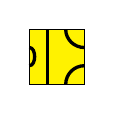
\begin{tikzpicture}[x=7mm,y=7mm]

\draw[black,fill=yellow] (0.000000,0.000000) rectangle (1.000000,-1.000000);
\draw[out=-90,in=90,looseness=1,very thick] (0.330000,0.000000) to (0.330000,-1.000000);
\draw[out=-90,in=180,looseness=1,very thick] (0.660000,0.000000) to (1.000000,-0.330000);
\draw[out=180,in=90,looseness=1,very thick] (1.000000,-0.660000) to (0.660000,-1.000000);
\draw[out=0,in=0,looseness=1,very thick] (0.000000,-0.660000) to (0.000000,-0.330000);
\end{tikzpicture}

\item Player 1 \textcolor{gray}{\LARGE$\bullet$} plays at row 3, col 1:
\begin{center}

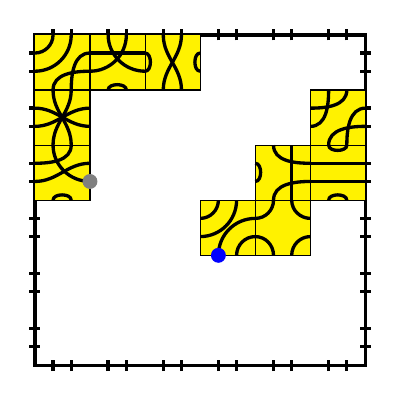
\begin{tikzpicture}[x=7mm,y=7mm]

\draw[very thick] (0.000000,0.000000) rectangle (6.000000,-6.000000);
\draw (0.000000,0.000000) grid[step=6] (6.000000,-6.000000);
\draw[very thick] (-0.100000,-0.330000) to (0.100000,-0.330000);
\draw[very thick] (5.900000,-0.330000) to (6.100000,-0.330000);
\draw[very thick] (0.330000,-0.100000) to (0.330000,0.100000);
\draw[very thick] (0.330000,-6.100000) to (0.330000,-5.900000);
\draw[very thick] (-0.100000,-0.660000) to (0.100000,-0.660000);
\draw[very thick] (5.900000,-0.660000) to (6.100000,-0.660000);
\draw[very thick] (0.660000,-0.100000) to (0.660000,0.100000);
\draw[very thick] (0.660000,-6.100000) to (0.660000,-5.900000);
\draw[very thick] (-0.100000,-1.330000) to (0.100000,-1.330000);
\draw[very thick] (5.900000,-1.330000) to (6.100000,-1.330000);
\draw[very thick] (1.330000,-0.100000) to (1.330000,0.100000);
\draw[very thick] (1.330000,-6.100000) to (1.330000,-5.900000);
\draw[very thick] (-0.100000,-1.660000) to (0.100000,-1.660000);
\draw[very thick] (5.900000,-1.660000) to (6.100000,-1.660000);
\draw[very thick] (1.660000,-0.100000) to (1.660000,0.100000);
\draw[very thick] (1.660000,-6.100000) to (1.660000,-5.900000);
\draw[very thick] (-0.100000,-2.330000) to (0.100000,-2.330000);
\draw[very thick] (5.900000,-2.330000) to (6.100000,-2.330000);
\draw[very thick] (2.330000,-0.100000) to (2.330000,0.100000);
\draw[very thick] (2.330000,-6.100000) to (2.330000,-5.900000);
\draw[very thick] (-0.100000,-2.660000) to (0.100000,-2.660000);
\draw[very thick] (5.900000,-2.660000) to (6.100000,-2.660000);
\draw[very thick] (2.660000,-0.100000) to (2.660000,0.100000);
\draw[very thick] (2.660000,-6.100000) to (2.660000,-5.900000);
\draw[very thick] (-0.100000,-3.330000) to (0.100000,-3.330000);
\draw[very thick] (5.900000,-3.330000) to (6.100000,-3.330000);
\draw[very thick] (3.330000,-0.100000) to (3.330000,0.100000);
\draw[very thick] (3.330000,-6.100000) to (3.330000,-5.900000);
\draw[very thick] (-0.100000,-3.660000) to (0.100000,-3.660000);
\draw[very thick] (5.900000,-3.660000) to (6.100000,-3.660000);
\draw[very thick] (3.660000,-0.100000) to (3.660000,0.100000);
\draw[very thick] (3.660000,-6.100000) to (3.660000,-5.900000);
\draw[very thick] (-0.100000,-4.330000) to (0.100000,-4.330000);
\draw[very thick] (5.900000,-4.330000) to (6.100000,-4.330000);
\draw[very thick] (4.330000,-0.100000) to (4.330000,0.100000);
\draw[very thick] (4.330000,-6.100000) to (4.330000,-5.900000);
\draw[very thick] (-0.100000,-4.660000) to (0.100000,-4.660000);
\draw[very thick] (5.900000,-4.660000) to (6.100000,-4.660000);
\draw[very thick] (4.660000,-0.100000) to (4.660000,0.100000);
\draw[very thick] (4.660000,-6.100000) to (4.660000,-5.900000);
\draw[very thick] (-0.100000,-5.330000) to (0.100000,-5.330000);
\draw[very thick] (5.900000,-5.330000) to (6.100000,-5.330000);
\draw[very thick] (5.330000,-0.100000) to (5.330000,0.100000);
\draw[very thick] (5.330000,-6.100000) to (5.330000,-5.900000);
\draw[very thick] (-0.100000,-5.660000) to (0.100000,-5.660000);
\draw[very thick] (5.900000,-5.660000) to (6.100000,-5.660000);
\draw[very thick] (5.660000,-0.100000) to (5.660000,0.100000);
\draw[very thick] (5.660000,-6.100000) to (5.660000,-5.900000);
\draw[black,fill=yellow] (0.000000,0.000000) rectangle (1.000000,-1.000000);
\draw[out=-90,in=0,looseness=1,very thick] (0.330000,0.000000) to (0.000000,-0.330000);
\draw[out=-90,in=0,looseness=1,very thick] (0.660000,0.000000) to (0.000000,-0.660000);
\draw[out=180,in=90,looseness=1,very thick] (1.000000,-0.330000) to (0.660000,-1.000000);
\draw[out=180,in=90,looseness=1,very thick] (1.000000,-0.660000) to (0.330000,-1.000000);
\draw[black,fill=yellow] (0.000000,-1.000000) rectangle (1.000000,-2.000000);
\draw[out=-90,in=90,looseness=1,very thick] (0.330000,-1.000000) to (0.660000,-2.000000);
\draw[out=-90,in=90,looseness=1,very thick] (0.660000,-1.000000) to (0.330000,-2.000000);
\draw[out=180,in=0,looseness=1,very thick] (1.000000,-1.330000) to (0.000000,-1.660000);
\draw[out=180,in=0,looseness=1,very thick] (1.000000,-1.660000) to (0.000000,-1.330000);
\draw[black,fill=yellow] (0.000000,-2.000000) rectangle (1.000000,-3.000000);
\draw[out=-90,in=180,looseness=1,very thick] (0.330000,-2.000000) to (1.000000,-2.660000);
\draw[out=-90,in=0,looseness=1,very thick] (0.660000,-2.000000) to (0.000000,-2.330000);
\draw[out=180,in=0,looseness=1,very thick] (1.000000,-2.330000) to (0.000000,-2.660000);
\draw[out=90,in=90,looseness=1,very thick] (0.660000,-3.000000) to (0.330000,-3.000000);
\draw[black,fill=yellow] (1.000000,0.000000) rectangle (2.000000,-1.000000);
\draw[out=-90,in=180,looseness=1,very thick] (1.330000,0.000000) to (2.000000,-0.660000);
\draw[out=-90,in=0,looseness=1,very thick] (1.660000,0.000000) to (1.000000,-0.660000);
\draw[out=180,in=0,looseness=1,very thick] (2.000000,-0.330000) to (1.000000,-0.330000);
\draw[out=90,in=90,looseness=1,very thick] (1.660000,-1.000000) to (1.330000,-1.000000);
\draw[black,fill=yellow] (2.000000,0.000000) rectangle (3.000000,-1.000000);
\draw[out=-90,in=90,looseness=1,very thick] (2.330000,0.000000) to (2.660000,-1.000000);
\draw[out=-90,in=90,looseness=1,very thick] (2.660000,0.000000) to (2.330000,-1.000000);
\draw[out=180,in=180,looseness=1,very thick] (3.000000,-0.330000) to (3.000000,-0.660000);
\draw[out=0,in=0,looseness=1,very thick] (2.000000,-0.660000) to (2.000000,-0.330000);
\draw[black,fill=yellow] (3.000000,-3.000000) rectangle (4.000000,-4.000000);
\draw[out=-90,in=0,looseness=1,very thick] (3.330000,-3.000000) to (3.000000,-3.330000);
\draw[out=-90,in=0,looseness=1,very thick] (3.660000,-3.000000) to (3.000000,-3.660000);
\draw[out=180,in=90,looseness=1,very thick] (4.000000,-3.330000) to (3.330000,-4.000000);
\draw[out=180,in=90,looseness=1,very thick] (4.000000,-3.660000) to (3.660000,-4.000000);
\draw[black,fill=yellow] (4.000000,-2.000000) rectangle (5.000000,-3.000000);
\draw[out=-90,in=180,looseness=1,very thick] (4.330000,-2.000000) to (5.000000,-2.330000);
\draw[out=-90,in=90,looseness=1,very thick] (4.660000,-2.000000) to (4.660000,-3.000000);
\draw[out=180,in=90,looseness=1,very thick] (5.000000,-2.660000) to (4.330000,-3.000000);
\draw[out=0,in=0,looseness=1,very thick] (4.000000,-2.660000) to (4.000000,-2.330000);
\draw[black,fill=yellow] (4.000000,-3.000000) rectangle (5.000000,-4.000000);
\draw[out=-90,in=0,looseness=1,very thick] (4.330000,-3.000000) to (4.000000,-3.330000);
\draw[out=-90,in=180,looseness=1,very thick] (4.660000,-3.000000) to (5.000000,-3.330000);
\draw[out=180,in=90,looseness=1,very thick] (5.000000,-3.660000) to (4.660000,-4.000000);
\draw[out=90,in=0,looseness=1,very thick] (4.330000,-4.000000) to (4.000000,-3.660000);
\draw[black,fill=yellow] (5.000000,-1.000000) rectangle (6.000000,-2.000000);
\draw[out=-90,in=0,looseness=1,very thick] (5.330000,-1.000000) to (5.000000,-1.660000);
\draw[out=-90,in=0,looseness=1,very thick] (5.660000,-1.000000) to (5.000000,-1.330000);
\draw[out=180,in=90,looseness=1,very thick] (6.000000,-1.330000) to (5.660000,-2.000000);
\draw[out=180,in=90,looseness=1,very thick] (6.000000,-1.660000) to (5.330000,-2.000000);
\draw[black,fill=yellow] (5.000000,-2.000000) rectangle (6.000000,-3.000000);
\draw[out=-90,in=-90,looseness=1,very thick] (5.330000,-2.000000) to (5.660000,-2.000000);
\draw[out=180,in=0,looseness=1,very thick] (6.000000,-2.330000) to (5.000000,-2.330000);
\draw[out=180,in=0,looseness=1,very thick] (6.000000,-2.660000) to (5.000000,-2.660000);
\draw[out=90,in=90,looseness=1,very thick] (5.660000,-3.000000) to (5.330000,-3.000000);
\draw[draw=blue,fill=blue] (3.330000,-4.000000) circle [x radius=0.125000,y radius=0.125000];
\draw[draw=gray,fill=gray] (1.000000,-2.660000) circle [x radius=0.125000,y radius=0.125000];
\end{tikzpicture}

\end{center}

\item[(22)] Player 1 \textcolor{gray}{\LARGE$\bullet$} draws 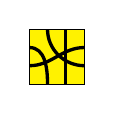
\begin{tikzpicture}[x=7mm,y=7mm]

\draw[black,fill=yellow] (0.000000,0.000000) rectangle (1.000000,-1.000000);
\draw[out=-90,in=180,looseness=1,very thick] (0.330000,0.000000) to (1.000000,-0.660000);
\draw[out=-90,in=90,looseness=1,very thick] (0.660000,0.000000) to (0.660000,-1.000000);
\draw[out=180,in=0,looseness=1,very thick] (1.000000,-0.330000) to (0.000000,-0.660000);
\draw[out=90,in=0,looseness=1,very thick] (0.330000,-1.000000) to (0.000000,-0.330000);
\end{tikzpicture}

\item Player 2 \textcolor{blue}{\LARGE$\bullet$} plays at row 5, col 4:
\begin{center}

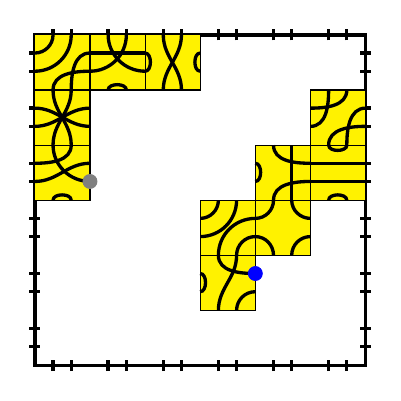
\begin{tikzpicture}[x=7mm,y=7mm]

\draw[very thick] (0.000000,0.000000) rectangle (6.000000,-6.000000);
\draw (0.000000,0.000000) grid[step=6] (6.000000,-6.000000);
\draw[very thick] (-0.100000,-0.330000) to (0.100000,-0.330000);
\draw[very thick] (5.900000,-0.330000) to (6.100000,-0.330000);
\draw[very thick] (0.330000,-0.100000) to (0.330000,0.100000);
\draw[very thick] (0.330000,-6.100000) to (0.330000,-5.900000);
\draw[very thick] (-0.100000,-0.660000) to (0.100000,-0.660000);
\draw[very thick] (5.900000,-0.660000) to (6.100000,-0.660000);
\draw[very thick] (0.660000,-0.100000) to (0.660000,0.100000);
\draw[very thick] (0.660000,-6.100000) to (0.660000,-5.900000);
\draw[very thick] (-0.100000,-1.330000) to (0.100000,-1.330000);
\draw[very thick] (5.900000,-1.330000) to (6.100000,-1.330000);
\draw[very thick] (1.330000,-0.100000) to (1.330000,0.100000);
\draw[very thick] (1.330000,-6.100000) to (1.330000,-5.900000);
\draw[very thick] (-0.100000,-1.660000) to (0.100000,-1.660000);
\draw[very thick] (5.900000,-1.660000) to (6.100000,-1.660000);
\draw[very thick] (1.660000,-0.100000) to (1.660000,0.100000);
\draw[very thick] (1.660000,-6.100000) to (1.660000,-5.900000);
\draw[very thick] (-0.100000,-2.330000) to (0.100000,-2.330000);
\draw[very thick] (5.900000,-2.330000) to (6.100000,-2.330000);
\draw[very thick] (2.330000,-0.100000) to (2.330000,0.100000);
\draw[very thick] (2.330000,-6.100000) to (2.330000,-5.900000);
\draw[very thick] (-0.100000,-2.660000) to (0.100000,-2.660000);
\draw[very thick] (5.900000,-2.660000) to (6.100000,-2.660000);
\draw[very thick] (2.660000,-0.100000) to (2.660000,0.100000);
\draw[very thick] (2.660000,-6.100000) to (2.660000,-5.900000);
\draw[very thick] (-0.100000,-3.330000) to (0.100000,-3.330000);
\draw[very thick] (5.900000,-3.330000) to (6.100000,-3.330000);
\draw[very thick] (3.330000,-0.100000) to (3.330000,0.100000);
\draw[very thick] (3.330000,-6.100000) to (3.330000,-5.900000);
\draw[very thick] (-0.100000,-3.660000) to (0.100000,-3.660000);
\draw[very thick] (5.900000,-3.660000) to (6.100000,-3.660000);
\draw[very thick] (3.660000,-0.100000) to (3.660000,0.100000);
\draw[very thick] (3.660000,-6.100000) to (3.660000,-5.900000);
\draw[very thick] (-0.100000,-4.330000) to (0.100000,-4.330000);
\draw[very thick] (5.900000,-4.330000) to (6.100000,-4.330000);
\draw[very thick] (4.330000,-0.100000) to (4.330000,0.100000);
\draw[very thick] (4.330000,-6.100000) to (4.330000,-5.900000);
\draw[very thick] (-0.100000,-4.660000) to (0.100000,-4.660000);
\draw[very thick] (5.900000,-4.660000) to (6.100000,-4.660000);
\draw[very thick] (4.660000,-0.100000) to (4.660000,0.100000);
\draw[very thick] (4.660000,-6.100000) to (4.660000,-5.900000);
\draw[very thick] (-0.100000,-5.330000) to (0.100000,-5.330000);
\draw[very thick] (5.900000,-5.330000) to (6.100000,-5.330000);
\draw[very thick] (5.330000,-0.100000) to (5.330000,0.100000);
\draw[very thick] (5.330000,-6.100000) to (5.330000,-5.900000);
\draw[very thick] (-0.100000,-5.660000) to (0.100000,-5.660000);
\draw[very thick] (5.900000,-5.660000) to (6.100000,-5.660000);
\draw[very thick] (5.660000,-0.100000) to (5.660000,0.100000);
\draw[very thick] (5.660000,-6.100000) to (5.660000,-5.900000);
\draw[black,fill=yellow] (0.000000,0.000000) rectangle (1.000000,-1.000000);
\draw[out=-90,in=0,looseness=1,very thick] (0.330000,0.000000) to (0.000000,-0.330000);
\draw[out=-90,in=0,looseness=1,very thick] (0.660000,0.000000) to (0.000000,-0.660000);
\draw[out=180,in=90,looseness=1,very thick] (1.000000,-0.330000) to (0.660000,-1.000000);
\draw[out=180,in=90,looseness=1,very thick] (1.000000,-0.660000) to (0.330000,-1.000000);
\draw[black,fill=yellow] (0.000000,-1.000000) rectangle (1.000000,-2.000000);
\draw[out=-90,in=90,looseness=1,very thick] (0.330000,-1.000000) to (0.660000,-2.000000);
\draw[out=-90,in=90,looseness=1,very thick] (0.660000,-1.000000) to (0.330000,-2.000000);
\draw[out=180,in=0,looseness=1,very thick] (1.000000,-1.330000) to (0.000000,-1.660000);
\draw[out=180,in=0,looseness=1,very thick] (1.000000,-1.660000) to (0.000000,-1.330000);
\draw[black,fill=yellow] (0.000000,-2.000000) rectangle (1.000000,-3.000000);
\draw[out=-90,in=180,looseness=1,very thick] (0.330000,-2.000000) to (1.000000,-2.660000);
\draw[out=-90,in=0,looseness=1,very thick] (0.660000,-2.000000) to (0.000000,-2.330000);
\draw[out=180,in=0,looseness=1,very thick] (1.000000,-2.330000) to (0.000000,-2.660000);
\draw[out=90,in=90,looseness=1,very thick] (0.660000,-3.000000) to (0.330000,-3.000000);
\draw[black,fill=yellow] (1.000000,0.000000) rectangle (2.000000,-1.000000);
\draw[out=-90,in=180,looseness=1,very thick] (1.330000,0.000000) to (2.000000,-0.660000);
\draw[out=-90,in=0,looseness=1,very thick] (1.660000,0.000000) to (1.000000,-0.660000);
\draw[out=180,in=0,looseness=1,very thick] (2.000000,-0.330000) to (1.000000,-0.330000);
\draw[out=90,in=90,looseness=1,very thick] (1.660000,-1.000000) to (1.330000,-1.000000);
\draw[black,fill=yellow] (2.000000,0.000000) rectangle (3.000000,-1.000000);
\draw[out=-90,in=90,looseness=1,very thick] (2.330000,0.000000) to (2.660000,-1.000000);
\draw[out=-90,in=90,looseness=1,very thick] (2.660000,0.000000) to (2.330000,-1.000000);
\draw[out=180,in=180,looseness=1,very thick] (3.000000,-0.330000) to (3.000000,-0.660000);
\draw[out=0,in=0,looseness=1,very thick] (2.000000,-0.660000) to (2.000000,-0.330000);
\draw[black,fill=yellow] (3.000000,-3.000000) rectangle (4.000000,-4.000000);
\draw[out=-90,in=0,looseness=1,very thick] (3.330000,-3.000000) to (3.000000,-3.330000);
\draw[out=-90,in=0,looseness=1,very thick] (3.660000,-3.000000) to (3.000000,-3.660000);
\draw[out=180,in=90,looseness=1,very thick] (4.000000,-3.330000) to (3.330000,-4.000000);
\draw[out=180,in=90,looseness=1,very thick] (4.000000,-3.660000) to (3.660000,-4.000000);
\draw[black,fill=yellow] (3.000000,-4.000000) rectangle (4.000000,-5.000000);
\draw[out=-90,in=180,looseness=1,very thick] (3.330000,-4.000000) to (4.000000,-4.330000);
\draw[out=-90,in=90,looseness=1,very thick] (3.660000,-4.000000) to (3.330000,-5.000000);
\draw[out=180,in=90,looseness=1,very thick] (4.000000,-4.660000) to (3.660000,-5.000000);
\draw[out=0,in=0,looseness=1,very thick] (3.000000,-4.660000) to (3.000000,-4.330000);
\draw[black,fill=yellow] (4.000000,-2.000000) rectangle (5.000000,-3.000000);
\draw[out=-90,in=180,looseness=1,very thick] (4.330000,-2.000000) to (5.000000,-2.330000);
\draw[out=-90,in=90,looseness=1,very thick] (4.660000,-2.000000) to (4.660000,-3.000000);
\draw[out=180,in=90,looseness=1,very thick] (5.000000,-2.660000) to (4.330000,-3.000000);
\draw[out=0,in=0,looseness=1,very thick] (4.000000,-2.660000) to (4.000000,-2.330000);
\draw[black,fill=yellow] (4.000000,-3.000000) rectangle (5.000000,-4.000000);
\draw[out=-90,in=0,looseness=1,very thick] (4.330000,-3.000000) to (4.000000,-3.330000);
\draw[out=-90,in=180,looseness=1,very thick] (4.660000,-3.000000) to (5.000000,-3.330000);
\draw[out=180,in=90,looseness=1,very thick] (5.000000,-3.660000) to (4.660000,-4.000000);
\draw[out=90,in=0,looseness=1,very thick] (4.330000,-4.000000) to (4.000000,-3.660000);
\draw[black,fill=yellow] (5.000000,-1.000000) rectangle (6.000000,-2.000000);
\draw[out=-90,in=0,looseness=1,very thick] (5.330000,-1.000000) to (5.000000,-1.660000);
\draw[out=-90,in=0,looseness=1,very thick] (5.660000,-1.000000) to (5.000000,-1.330000);
\draw[out=180,in=90,looseness=1,very thick] (6.000000,-1.330000) to (5.660000,-2.000000);
\draw[out=180,in=90,looseness=1,very thick] (6.000000,-1.660000) to (5.330000,-2.000000);
\draw[black,fill=yellow] (5.000000,-2.000000) rectangle (6.000000,-3.000000);
\draw[out=-90,in=-90,looseness=1,very thick] (5.330000,-2.000000) to (5.660000,-2.000000);
\draw[out=180,in=0,looseness=1,very thick] (6.000000,-2.330000) to (5.000000,-2.330000);
\draw[out=180,in=0,looseness=1,very thick] (6.000000,-2.660000) to (5.000000,-2.660000);
\draw[out=90,in=90,looseness=1,very thick] (5.660000,-3.000000) to (5.330000,-3.000000);
\draw[draw=blue,fill=blue] (4.000000,-4.330000) circle [x radius=0.125000,y radius=0.125000];
\draw[draw=gray,fill=gray] (1.000000,-2.660000) circle [x radius=0.125000,y radius=0.125000];
\end{tikzpicture}

\end{center}

\item[(23)] Player 2 \textcolor{blue}{\LARGE$\bullet$} draws 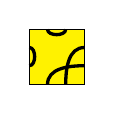
\begin{tikzpicture}[x=7mm,y=7mm]

\draw[black,fill=yellow] (0.000000,0.000000) rectangle (1.000000,-1.000000);
\draw[out=-90,in=-90,looseness=1,very thick] (0.330000,0.000000) to (0.660000,0.000000);
\draw[out=180,in=90,looseness=1,very thick] (1.000000,-0.330000) to (0.660000,-1.000000);
\draw[out=180,in=90,looseness=1,very thick] (1.000000,-0.660000) to (0.330000,-1.000000);
\draw[out=0,in=0,looseness=1,very thick] (0.000000,-0.660000) to (0.000000,-0.330000);
\end{tikzpicture}

\item Player 1 \textcolor{gray}{\LARGE$\bullet$} plays at row 3, col 2:
\begin{center}

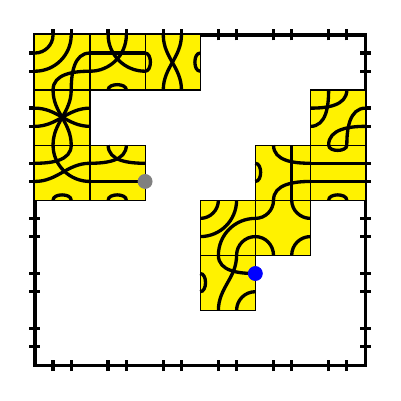
\begin{tikzpicture}[x=7mm,y=7mm]

\draw[very thick] (0.000000,0.000000) rectangle (6.000000,-6.000000);
\draw (0.000000,0.000000) grid[step=6] (6.000000,-6.000000);
\draw[very thick] (-0.100000,-0.330000) to (0.100000,-0.330000);
\draw[very thick] (5.900000,-0.330000) to (6.100000,-0.330000);
\draw[very thick] (0.330000,-0.100000) to (0.330000,0.100000);
\draw[very thick] (0.330000,-6.100000) to (0.330000,-5.900000);
\draw[very thick] (-0.100000,-0.660000) to (0.100000,-0.660000);
\draw[very thick] (5.900000,-0.660000) to (6.100000,-0.660000);
\draw[very thick] (0.660000,-0.100000) to (0.660000,0.100000);
\draw[very thick] (0.660000,-6.100000) to (0.660000,-5.900000);
\draw[very thick] (-0.100000,-1.330000) to (0.100000,-1.330000);
\draw[very thick] (5.900000,-1.330000) to (6.100000,-1.330000);
\draw[very thick] (1.330000,-0.100000) to (1.330000,0.100000);
\draw[very thick] (1.330000,-6.100000) to (1.330000,-5.900000);
\draw[very thick] (-0.100000,-1.660000) to (0.100000,-1.660000);
\draw[very thick] (5.900000,-1.660000) to (6.100000,-1.660000);
\draw[very thick] (1.660000,-0.100000) to (1.660000,0.100000);
\draw[very thick] (1.660000,-6.100000) to (1.660000,-5.900000);
\draw[very thick] (-0.100000,-2.330000) to (0.100000,-2.330000);
\draw[very thick] (5.900000,-2.330000) to (6.100000,-2.330000);
\draw[very thick] (2.330000,-0.100000) to (2.330000,0.100000);
\draw[very thick] (2.330000,-6.100000) to (2.330000,-5.900000);
\draw[very thick] (-0.100000,-2.660000) to (0.100000,-2.660000);
\draw[very thick] (5.900000,-2.660000) to (6.100000,-2.660000);
\draw[very thick] (2.660000,-0.100000) to (2.660000,0.100000);
\draw[very thick] (2.660000,-6.100000) to (2.660000,-5.900000);
\draw[very thick] (-0.100000,-3.330000) to (0.100000,-3.330000);
\draw[very thick] (5.900000,-3.330000) to (6.100000,-3.330000);
\draw[very thick] (3.330000,-0.100000) to (3.330000,0.100000);
\draw[very thick] (3.330000,-6.100000) to (3.330000,-5.900000);
\draw[very thick] (-0.100000,-3.660000) to (0.100000,-3.660000);
\draw[very thick] (5.900000,-3.660000) to (6.100000,-3.660000);
\draw[very thick] (3.660000,-0.100000) to (3.660000,0.100000);
\draw[very thick] (3.660000,-6.100000) to (3.660000,-5.900000);
\draw[very thick] (-0.100000,-4.330000) to (0.100000,-4.330000);
\draw[very thick] (5.900000,-4.330000) to (6.100000,-4.330000);
\draw[very thick] (4.330000,-0.100000) to (4.330000,0.100000);
\draw[very thick] (4.330000,-6.100000) to (4.330000,-5.900000);
\draw[very thick] (-0.100000,-4.660000) to (0.100000,-4.660000);
\draw[very thick] (5.900000,-4.660000) to (6.100000,-4.660000);
\draw[very thick] (4.660000,-0.100000) to (4.660000,0.100000);
\draw[very thick] (4.660000,-6.100000) to (4.660000,-5.900000);
\draw[very thick] (-0.100000,-5.330000) to (0.100000,-5.330000);
\draw[very thick] (5.900000,-5.330000) to (6.100000,-5.330000);
\draw[very thick] (5.330000,-0.100000) to (5.330000,0.100000);
\draw[very thick] (5.330000,-6.100000) to (5.330000,-5.900000);
\draw[very thick] (-0.100000,-5.660000) to (0.100000,-5.660000);
\draw[very thick] (5.900000,-5.660000) to (6.100000,-5.660000);
\draw[very thick] (5.660000,-0.100000) to (5.660000,0.100000);
\draw[very thick] (5.660000,-6.100000) to (5.660000,-5.900000);
\draw[black,fill=yellow] (0.000000,0.000000) rectangle (1.000000,-1.000000);
\draw[out=-90,in=0,looseness=1,very thick] (0.330000,0.000000) to (0.000000,-0.330000);
\draw[out=-90,in=0,looseness=1,very thick] (0.660000,0.000000) to (0.000000,-0.660000);
\draw[out=180,in=90,looseness=1,very thick] (1.000000,-0.330000) to (0.660000,-1.000000);
\draw[out=180,in=90,looseness=1,very thick] (1.000000,-0.660000) to (0.330000,-1.000000);
\draw[black,fill=yellow] (0.000000,-1.000000) rectangle (1.000000,-2.000000);
\draw[out=-90,in=90,looseness=1,very thick] (0.330000,-1.000000) to (0.660000,-2.000000);
\draw[out=-90,in=90,looseness=1,very thick] (0.660000,-1.000000) to (0.330000,-2.000000);
\draw[out=180,in=0,looseness=1,very thick] (1.000000,-1.330000) to (0.000000,-1.660000);
\draw[out=180,in=0,looseness=1,very thick] (1.000000,-1.660000) to (0.000000,-1.330000);
\draw[black,fill=yellow] (0.000000,-2.000000) rectangle (1.000000,-3.000000);
\draw[out=-90,in=180,looseness=1,very thick] (0.330000,-2.000000) to (1.000000,-2.660000);
\draw[out=-90,in=0,looseness=1,very thick] (0.660000,-2.000000) to (0.000000,-2.330000);
\draw[out=180,in=0,looseness=1,very thick] (1.000000,-2.330000) to (0.000000,-2.660000);
\draw[out=90,in=90,looseness=1,very thick] (0.660000,-3.000000) to (0.330000,-3.000000);
\draw[black,fill=yellow] (1.000000,0.000000) rectangle (2.000000,-1.000000);
\draw[out=-90,in=180,looseness=1,very thick] (1.330000,0.000000) to (2.000000,-0.660000);
\draw[out=-90,in=0,looseness=1,very thick] (1.660000,0.000000) to (1.000000,-0.660000);
\draw[out=180,in=0,looseness=1,very thick] (2.000000,-0.330000) to (1.000000,-0.330000);
\draw[out=90,in=90,looseness=1,very thick] (1.660000,-1.000000) to (1.330000,-1.000000);
\draw[black,fill=yellow] (1.000000,-2.000000) rectangle (2.000000,-3.000000);
\draw[out=-90,in=180,looseness=1,very thick] (1.330000,-2.000000) to (2.000000,-2.330000);
\draw[out=-90,in=0,looseness=1,very thick] (1.660000,-2.000000) to (1.000000,-2.330000);
\draw[out=180,in=0,looseness=1,very thick] (2.000000,-2.660000) to (1.000000,-2.660000);
\draw[out=90,in=90,looseness=1,very thick] (1.660000,-3.000000) to (1.330000,-3.000000);
\draw[black,fill=yellow] (2.000000,0.000000) rectangle (3.000000,-1.000000);
\draw[out=-90,in=90,looseness=1,very thick] (2.330000,0.000000) to (2.660000,-1.000000);
\draw[out=-90,in=90,looseness=1,very thick] (2.660000,0.000000) to (2.330000,-1.000000);
\draw[out=180,in=180,looseness=1,very thick] (3.000000,-0.330000) to (3.000000,-0.660000);
\draw[out=0,in=0,looseness=1,very thick] (2.000000,-0.660000) to (2.000000,-0.330000);
\draw[black,fill=yellow] (3.000000,-3.000000) rectangle (4.000000,-4.000000);
\draw[out=-90,in=0,looseness=1,very thick] (3.330000,-3.000000) to (3.000000,-3.330000);
\draw[out=-90,in=0,looseness=1,very thick] (3.660000,-3.000000) to (3.000000,-3.660000);
\draw[out=180,in=90,looseness=1,very thick] (4.000000,-3.330000) to (3.330000,-4.000000);
\draw[out=180,in=90,looseness=1,very thick] (4.000000,-3.660000) to (3.660000,-4.000000);
\draw[black,fill=yellow] (3.000000,-4.000000) rectangle (4.000000,-5.000000);
\draw[out=-90,in=180,looseness=1,very thick] (3.330000,-4.000000) to (4.000000,-4.330000);
\draw[out=-90,in=90,looseness=1,very thick] (3.660000,-4.000000) to (3.330000,-5.000000);
\draw[out=180,in=90,looseness=1,very thick] (4.000000,-4.660000) to (3.660000,-5.000000);
\draw[out=0,in=0,looseness=1,very thick] (3.000000,-4.660000) to (3.000000,-4.330000);
\draw[black,fill=yellow] (4.000000,-2.000000) rectangle (5.000000,-3.000000);
\draw[out=-90,in=180,looseness=1,very thick] (4.330000,-2.000000) to (5.000000,-2.330000);
\draw[out=-90,in=90,looseness=1,very thick] (4.660000,-2.000000) to (4.660000,-3.000000);
\draw[out=180,in=90,looseness=1,very thick] (5.000000,-2.660000) to (4.330000,-3.000000);
\draw[out=0,in=0,looseness=1,very thick] (4.000000,-2.660000) to (4.000000,-2.330000);
\draw[black,fill=yellow] (4.000000,-3.000000) rectangle (5.000000,-4.000000);
\draw[out=-90,in=0,looseness=1,very thick] (4.330000,-3.000000) to (4.000000,-3.330000);
\draw[out=-90,in=180,looseness=1,very thick] (4.660000,-3.000000) to (5.000000,-3.330000);
\draw[out=180,in=90,looseness=1,very thick] (5.000000,-3.660000) to (4.660000,-4.000000);
\draw[out=90,in=0,looseness=1,very thick] (4.330000,-4.000000) to (4.000000,-3.660000);
\draw[black,fill=yellow] (5.000000,-1.000000) rectangle (6.000000,-2.000000);
\draw[out=-90,in=0,looseness=1,very thick] (5.330000,-1.000000) to (5.000000,-1.660000);
\draw[out=-90,in=0,looseness=1,very thick] (5.660000,-1.000000) to (5.000000,-1.330000);
\draw[out=180,in=90,looseness=1,very thick] (6.000000,-1.330000) to (5.660000,-2.000000);
\draw[out=180,in=90,looseness=1,very thick] (6.000000,-1.660000) to (5.330000,-2.000000);
\draw[black,fill=yellow] (5.000000,-2.000000) rectangle (6.000000,-3.000000);
\draw[out=-90,in=-90,looseness=1,very thick] (5.330000,-2.000000) to (5.660000,-2.000000);
\draw[out=180,in=0,looseness=1,very thick] (6.000000,-2.330000) to (5.000000,-2.330000);
\draw[out=180,in=0,looseness=1,very thick] (6.000000,-2.660000) to (5.000000,-2.660000);
\draw[out=90,in=90,looseness=1,very thick] (5.660000,-3.000000) to (5.330000,-3.000000);
\draw[draw=blue,fill=blue] (4.000000,-4.330000) circle [x radius=0.125000,y radius=0.125000];
\draw[draw=gray,fill=gray] (2.000000,-2.660000) circle [x radius=0.125000,y radius=0.125000];
\end{tikzpicture}

\end{center}

\item[(24)] Player 1 \textcolor{gray}{\LARGE$\bullet$} draws 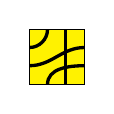
\begin{tikzpicture}[x=7mm,y=7mm]

\draw[black,fill=yellow] (0.000000,0.000000) rectangle (1.000000,-1.000000);
\draw[out=-90,in=0,looseness=1,very thick] (0.330000,0.000000) to (0.000000,-0.330000);
\draw[out=-90,in=90,looseness=1,very thick] (0.660000,0.000000) to (0.660000,-1.000000);
\draw[out=180,in=0,looseness=1,very thick] (1.000000,-0.330000) to (0.000000,-0.660000);
\draw[out=180,in=90,looseness=1,very thick] (1.000000,-0.660000) to (0.330000,-1.000000);
\end{tikzpicture}

\item Player 2 \textcolor{blue}{\LARGE$\bullet$} plays at row 5, col 5:
\begin{center}

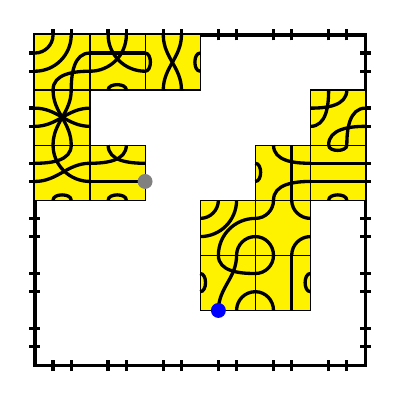
\begin{tikzpicture}[x=7mm,y=7mm]

\draw[very thick] (0.000000,0.000000) rectangle (6.000000,-6.000000);
\draw (0.000000,0.000000) grid[step=6] (6.000000,-6.000000);
\draw[very thick] (-0.100000,-0.330000) to (0.100000,-0.330000);
\draw[very thick] (5.900000,-0.330000) to (6.100000,-0.330000);
\draw[very thick] (0.330000,-0.100000) to (0.330000,0.100000);
\draw[very thick] (0.330000,-6.100000) to (0.330000,-5.900000);
\draw[very thick] (-0.100000,-0.660000) to (0.100000,-0.660000);
\draw[very thick] (5.900000,-0.660000) to (6.100000,-0.660000);
\draw[very thick] (0.660000,-0.100000) to (0.660000,0.100000);
\draw[very thick] (0.660000,-6.100000) to (0.660000,-5.900000);
\draw[very thick] (-0.100000,-1.330000) to (0.100000,-1.330000);
\draw[very thick] (5.900000,-1.330000) to (6.100000,-1.330000);
\draw[very thick] (1.330000,-0.100000) to (1.330000,0.100000);
\draw[very thick] (1.330000,-6.100000) to (1.330000,-5.900000);
\draw[very thick] (-0.100000,-1.660000) to (0.100000,-1.660000);
\draw[very thick] (5.900000,-1.660000) to (6.100000,-1.660000);
\draw[very thick] (1.660000,-0.100000) to (1.660000,0.100000);
\draw[very thick] (1.660000,-6.100000) to (1.660000,-5.900000);
\draw[very thick] (-0.100000,-2.330000) to (0.100000,-2.330000);
\draw[very thick] (5.900000,-2.330000) to (6.100000,-2.330000);
\draw[very thick] (2.330000,-0.100000) to (2.330000,0.100000);
\draw[very thick] (2.330000,-6.100000) to (2.330000,-5.900000);
\draw[very thick] (-0.100000,-2.660000) to (0.100000,-2.660000);
\draw[very thick] (5.900000,-2.660000) to (6.100000,-2.660000);
\draw[very thick] (2.660000,-0.100000) to (2.660000,0.100000);
\draw[very thick] (2.660000,-6.100000) to (2.660000,-5.900000);
\draw[very thick] (-0.100000,-3.330000) to (0.100000,-3.330000);
\draw[very thick] (5.900000,-3.330000) to (6.100000,-3.330000);
\draw[very thick] (3.330000,-0.100000) to (3.330000,0.100000);
\draw[very thick] (3.330000,-6.100000) to (3.330000,-5.900000);
\draw[very thick] (-0.100000,-3.660000) to (0.100000,-3.660000);
\draw[very thick] (5.900000,-3.660000) to (6.100000,-3.660000);
\draw[very thick] (3.660000,-0.100000) to (3.660000,0.100000);
\draw[very thick] (3.660000,-6.100000) to (3.660000,-5.900000);
\draw[very thick] (-0.100000,-4.330000) to (0.100000,-4.330000);
\draw[very thick] (5.900000,-4.330000) to (6.100000,-4.330000);
\draw[very thick] (4.330000,-0.100000) to (4.330000,0.100000);
\draw[very thick] (4.330000,-6.100000) to (4.330000,-5.900000);
\draw[very thick] (-0.100000,-4.660000) to (0.100000,-4.660000);
\draw[very thick] (5.900000,-4.660000) to (6.100000,-4.660000);
\draw[very thick] (4.660000,-0.100000) to (4.660000,0.100000);
\draw[very thick] (4.660000,-6.100000) to (4.660000,-5.900000);
\draw[very thick] (-0.100000,-5.330000) to (0.100000,-5.330000);
\draw[very thick] (5.900000,-5.330000) to (6.100000,-5.330000);
\draw[very thick] (5.330000,-0.100000) to (5.330000,0.100000);
\draw[very thick] (5.330000,-6.100000) to (5.330000,-5.900000);
\draw[very thick] (-0.100000,-5.660000) to (0.100000,-5.660000);
\draw[very thick] (5.900000,-5.660000) to (6.100000,-5.660000);
\draw[very thick] (5.660000,-0.100000) to (5.660000,0.100000);
\draw[very thick] (5.660000,-6.100000) to (5.660000,-5.900000);
\draw[black,fill=yellow] (0.000000,0.000000) rectangle (1.000000,-1.000000);
\draw[out=-90,in=0,looseness=1,very thick] (0.330000,0.000000) to (0.000000,-0.330000);
\draw[out=-90,in=0,looseness=1,very thick] (0.660000,0.000000) to (0.000000,-0.660000);
\draw[out=180,in=90,looseness=1,very thick] (1.000000,-0.330000) to (0.660000,-1.000000);
\draw[out=180,in=90,looseness=1,very thick] (1.000000,-0.660000) to (0.330000,-1.000000);
\draw[black,fill=yellow] (0.000000,-1.000000) rectangle (1.000000,-2.000000);
\draw[out=-90,in=90,looseness=1,very thick] (0.330000,-1.000000) to (0.660000,-2.000000);
\draw[out=-90,in=90,looseness=1,very thick] (0.660000,-1.000000) to (0.330000,-2.000000);
\draw[out=180,in=0,looseness=1,very thick] (1.000000,-1.330000) to (0.000000,-1.660000);
\draw[out=180,in=0,looseness=1,very thick] (1.000000,-1.660000) to (0.000000,-1.330000);
\draw[black,fill=yellow] (0.000000,-2.000000) rectangle (1.000000,-3.000000);
\draw[out=-90,in=180,looseness=1,very thick] (0.330000,-2.000000) to (1.000000,-2.660000);
\draw[out=-90,in=0,looseness=1,very thick] (0.660000,-2.000000) to (0.000000,-2.330000);
\draw[out=180,in=0,looseness=1,very thick] (1.000000,-2.330000) to (0.000000,-2.660000);
\draw[out=90,in=90,looseness=1,very thick] (0.660000,-3.000000) to (0.330000,-3.000000);
\draw[black,fill=yellow] (1.000000,0.000000) rectangle (2.000000,-1.000000);
\draw[out=-90,in=180,looseness=1,very thick] (1.330000,0.000000) to (2.000000,-0.660000);
\draw[out=-90,in=0,looseness=1,very thick] (1.660000,0.000000) to (1.000000,-0.660000);
\draw[out=180,in=0,looseness=1,very thick] (2.000000,-0.330000) to (1.000000,-0.330000);
\draw[out=90,in=90,looseness=1,very thick] (1.660000,-1.000000) to (1.330000,-1.000000);
\draw[black,fill=yellow] (1.000000,-2.000000) rectangle (2.000000,-3.000000);
\draw[out=-90,in=180,looseness=1,very thick] (1.330000,-2.000000) to (2.000000,-2.330000);
\draw[out=-90,in=0,looseness=1,very thick] (1.660000,-2.000000) to (1.000000,-2.330000);
\draw[out=180,in=0,looseness=1,very thick] (2.000000,-2.660000) to (1.000000,-2.660000);
\draw[out=90,in=90,looseness=1,very thick] (1.660000,-3.000000) to (1.330000,-3.000000);
\draw[black,fill=yellow] (2.000000,0.000000) rectangle (3.000000,-1.000000);
\draw[out=-90,in=90,looseness=1,very thick] (2.330000,0.000000) to (2.660000,-1.000000);
\draw[out=-90,in=90,looseness=1,very thick] (2.660000,0.000000) to (2.330000,-1.000000);
\draw[out=180,in=180,looseness=1,very thick] (3.000000,-0.330000) to (3.000000,-0.660000);
\draw[out=0,in=0,looseness=1,very thick] (2.000000,-0.660000) to (2.000000,-0.330000);
\draw[black,fill=yellow] (3.000000,-3.000000) rectangle (4.000000,-4.000000);
\draw[out=-90,in=0,looseness=1,very thick] (3.330000,-3.000000) to (3.000000,-3.330000);
\draw[out=-90,in=0,looseness=1,very thick] (3.660000,-3.000000) to (3.000000,-3.660000);
\draw[out=180,in=90,looseness=1,very thick] (4.000000,-3.330000) to (3.330000,-4.000000);
\draw[out=180,in=90,looseness=1,very thick] (4.000000,-3.660000) to (3.660000,-4.000000);
\draw[black,fill=yellow] (3.000000,-4.000000) rectangle (4.000000,-5.000000);
\draw[out=-90,in=180,looseness=1,very thick] (3.330000,-4.000000) to (4.000000,-4.330000);
\draw[out=-90,in=90,looseness=1,very thick] (3.660000,-4.000000) to (3.330000,-5.000000);
\draw[out=180,in=90,looseness=1,very thick] (4.000000,-4.660000) to (3.660000,-5.000000);
\draw[out=0,in=0,looseness=1,very thick] (3.000000,-4.660000) to (3.000000,-4.330000);
\draw[black,fill=yellow] (4.000000,-2.000000) rectangle (5.000000,-3.000000);
\draw[out=-90,in=180,looseness=1,very thick] (4.330000,-2.000000) to (5.000000,-2.330000);
\draw[out=-90,in=90,looseness=1,very thick] (4.660000,-2.000000) to (4.660000,-3.000000);
\draw[out=180,in=90,looseness=1,very thick] (5.000000,-2.660000) to (4.330000,-3.000000);
\draw[out=0,in=0,looseness=1,very thick] (4.000000,-2.660000) to (4.000000,-2.330000);
\draw[black,fill=yellow] (4.000000,-3.000000) rectangle (5.000000,-4.000000);
\draw[out=-90,in=0,looseness=1,very thick] (4.330000,-3.000000) to (4.000000,-3.330000);
\draw[out=-90,in=180,looseness=1,very thick] (4.660000,-3.000000) to (5.000000,-3.330000);
\draw[out=180,in=90,looseness=1,very thick] (5.000000,-3.660000) to (4.660000,-4.000000);
\draw[out=90,in=0,looseness=1,very thick] (4.330000,-4.000000) to (4.000000,-3.660000);
\draw[black,fill=yellow] (4.000000,-4.000000) rectangle (5.000000,-5.000000);
\draw[out=-90,in=0,looseness=1,very thick] (4.330000,-4.000000) to (4.000000,-4.330000);
\draw[out=-90,in=90,looseness=1,very thick] (4.660000,-4.000000) to (4.660000,-5.000000);
\draw[out=180,in=180,looseness=1,very thick] (5.000000,-4.330000) to (5.000000,-4.660000);
\draw[out=90,in=0,looseness=1,very thick] (4.330000,-5.000000) to (4.000000,-4.660000);
\draw[black,fill=yellow] (5.000000,-1.000000) rectangle (6.000000,-2.000000);
\draw[out=-90,in=0,looseness=1,very thick] (5.330000,-1.000000) to (5.000000,-1.660000);
\draw[out=-90,in=0,looseness=1,very thick] (5.660000,-1.000000) to (5.000000,-1.330000);
\draw[out=180,in=90,looseness=1,very thick] (6.000000,-1.330000) to (5.660000,-2.000000);
\draw[out=180,in=90,looseness=1,very thick] (6.000000,-1.660000) to (5.330000,-2.000000);
\draw[black,fill=yellow] (5.000000,-2.000000) rectangle (6.000000,-3.000000);
\draw[out=-90,in=-90,looseness=1,very thick] (5.330000,-2.000000) to (5.660000,-2.000000);
\draw[out=180,in=0,looseness=1,very thick] (6.000000,-2.330000) to (5.000000,-2.330000);
\draw[out=180,in=0,looseness=1,very thick] (6.000000,-2.660000) to (5.000000,-2.660000);
\draw[out=90,in=90,looseness=1,very thick] (5.660000,-3.000000) to (5.330000,-3.000000);
\draw[draw=blue,fill=blue] (3.330000,-5.000000) circle [x radius=0.125000,y radius=0.125000];
\draw[draw=gray,fill=gray] (2.000000,-2.660000) circle [x radius=0.125000,y radius=0.125000];
\end{tikzpicture}

\end{center}

\item[(25)] Player 2 \textcolor{blue}{\LARGE$\bullet$} draws 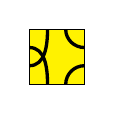
\begin{tikzpicture}[x=7mm,y=7mm]

\draw[black,fill=yellow] (0.000000,0.000000) rectangle (1.000000,-1.000000);
\draw[out=-90,in=0,looseness=1,very thick] (0.330000,0.000000) to (0.000000,-0.660000);
\draw[out=-90,in=180,looseness=1,very thick] (0.660000,0.000000) to (1.000000,-0.330000);
\draw[out=180,in=90,looseness=1,very thick] (1.000000,-0.660000) to (0.660000,-1.000000);
\draw[out=90,in=0,looseness=1,very thick] (0.330000,-1.000000) to (0.000000,-0.330000);
\end{tikzpicture}

\item Player 1 \textcolor{gray}{\LARGE$\bullet$} plays at row 3, col 3:
\begin{center}

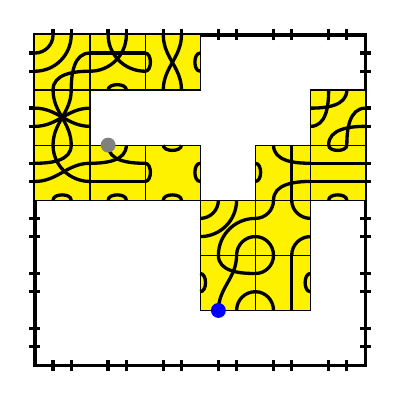
\begin{tikzpicture}[x=7mm,y=7mm]

\draw[very thick] (0.000000,0.000000) rectangle (6.000000,-6.000000);
\draw (0.000000,0.000000) grid[step=6] (6.000000,-6.000000);
\draw[very thick] (-0.100000,-0.330000) to (0.100000,-0.330000);
\draw[very thick] (5.900000,-0.330000) to (6.100000,-0.330000);
\draw[very thick] (0.330000,-0.100000) to (0.330000,0.100000);
\draw[very thick] (0.330000,-6.100000) to (0.330000,-5.900000);
\draw[very thick] (-0.100000,-0.660000) to (0.100000,-0.660000);
\draw[very thick] (5.900000,-0.660000) to (6.100000,-0.660000);
\draw[very thick] (0.660000,-0.100000) to (0.660000,0.100000);
\draw[very thick] (0.660000,-6.100000) to (0.660000,-5.900000);
\draw[very thick] (-0.100000,-1.330000) to (0.100000,-1.330000);
\draw[very thick] (5.900000,-1.330000) to (6.100000,-1.330000);
\draw[very thick] (1.330000,-0.100000) to (1.330000,0.100000);
\draw[very thick] (1.330000,-6.100000) to (1.330000,-5.900000);
\draw[very thick] (-0.100000,-1.660000) to (0.100000,-1.660000);
\draw[very thick] (5.900000,-1.660000) to (6.100000,-1.660000);
\draw[very thick] (1.660000,-0.100000) to (1.660000,0.100000);
\draw[very thick] (1.660000,-6.100000) to (1.660000,-5.900000);
\draw[very thick] (-0.100000,-2.330000) to (0.100000,-2.330000);
\draw[very thick] (5.900000,-2.330000) to (6.100000,-2.330000);
\draw[very thick] (2.330000,-0.100000) to (2.330000,0.100000);
\draw[very thick] (2.330000,-6.100000) to (2.330000,-5.900000);
\draw[very thick] (-0.100000,-2.660000) to (0.100000,-2.660000);
\draw[very thick] (5.900000,-2.660000) to (6.100000,-2.660000);
\draw[very thick] (2.660000,-0.100000) to (2.660000,0.100000);
\draw[very thick] (2.660000,-6.100000) to (2.660000,-5.900000);
\draw[very thick] (-0.100000,-3.330000) to (0.100000,-3.330000);
\draw[very thick] (5.900000,-3.330000) to (6.100000,-3.330000);
\draw[very thick] (3.330000,-0.100000) to (3.330000,0.100000);
\draw[very thick] (3.330000,-6.100000) to (3.330000,-5.900000);
\draw[very thick] (-0.100000,-3.660000) to (0.100000,-3.660000);
\draw[very thick] (5.900000,-3.660000) to (6.100000,-3.660000);
\draw[very thick] (3.660000,-0.100000) to (3.660000,0.100000);
\draw[very thick] (3.660000,-6.100000) to (3.660000,-5.900000);
\draw[very thick] (-0.100000,-4.330000) to (0.100000,-4.330000);
\draw[very thick] (5.900000,-4.330000) to (6.100000,-4.330000);
\draw[very thick] (4.330000,-0.100000) to (4.330000,0.100000);
\draw[very thick] (4.330000,-6.100000) to (4.330000,-5.900000);
\draw[very thick] (-0.100000,-4.660000) to (0.100000,-4.660000);
\draw[very thick] (5.900000,-4.660000) to (6.100000,-4.660000);
\draw[very thick] (4.660000,-0.100000) to (4.660000,0.100000);
\draw[very thick] (4.660000,-6.100000) to (4.660000,-5.900000);
\draw[very thick] (-0.100000,-5.330000) to (0.100000,-5.330000);
\draw[very thick] (5.900000,-5.330000) to (6.100000,-5.330000);
\draw[very thick] (5.330000,-0.100000) to (5.330000,0.100000);
\draw[very thick] (5.330000,-6.100000) to (5.330000,-5.900000);
\draw[very thick] (-0.100000,-5.660000) to (0.100000,-5.660000);
\draw[very thick] (5.900000,-5.660000) to (6.100000,-5.660000);
\draw[very thick] (5.660000,-0.100000) to (5.660000,0.100000);
\draw[very thick] (5.660000,-6.100000) to (5.660000,-5.900000);
\draw[black,fill=yellow] (0.000000,0.000000) rectangle (1.000000,-1.000000);
\draw[out=-90,in=0,looseness=1,very thick] (0.330000,0.000000) to (0.000000,-0.330000);
\draw[out=-90,in=0,looseness=1,very thick] (0.660000,0.000000) to (0.000000,-0.660000);
\draw[out=180,in=90,looseness=1,very thick] (1.000000,-0.330000) to (0.660000,-1.000000);
\draw[out=180,in=90,looseness=1,very thick] (1.000000,-0.660000) to (0.330000,-1.000000);
\draw[black,fill=yellow] (0.000000,-1.000000) rectangle (1.000000,-2.000000);
\draw[out=-90,in=90,looseness=1,very thick] (0.330000,-1.000000) to (0.660000,-2.000000);
\draw[out=-90,in=90,looseness=1,very thick] (0.660000,-1.000000) to (0.330000,-2.000000);
\draw[out=180,in=0,looseness=1,very thick] (1.000000,-1.330000) to (0.000000,-1.660000);
\draw[out=180,in=0,looseness=1,very thick] (1.000000,-1.660000) to (0.000000,-1.330000);
\draw[black,fill=yellow] (0.000000,-2.000000) rectangle (1.000000,-3.000000);
\draw[out=-90,in=180,looseness=1,very thick] (0.330000,-2.000000) to (1.000000,-2.660000);
\draw[out=-90,in=0,looseness=1,very thick] (0.660000,-2.000000) to (0.000000,-2.330000);
\draw[out=180,in=0,looseness=1,very thick] (1.000000,-2.330000) to (0.000000,-2.660000);
\draw[out=90,in=90,looseness=1,very thick] (0.660000,-3.000000) to (0.330000,-3.000000);
\draw[black,fill=yellow] (1.000000,0.000000) rectangle (2.000000,-1.000000);
\draw[out=-90,in=180,looseness=1,very thick] (1.330000,0.000000) to (2.000000,-0.660000);
\draw[out=-90,in=0,looseness=1,very thick] (1.660000,0.000000) to (1.000000,-0.660000);
\draw[out=180,in=0,looseness=1,very thick] (2.000000,-0.330000) to (1.000000,-0.330000);
\draw[out=90,in=90,looseness=1,very thick] (1.660000,-1.000000) to (1.330000,-1.000000);
\draw[black,fill=yellow] (1.000000,-2.000000) rectangle (2.000000,-3.000000);
\draw[out=-90,in=180,looseness=1,very thick] (1.330000,-2.000000) to (2.000000,-2.330000);
\draw[out=-90,in=0,looseness=1,very thick] (1.660000,-2.000000) to (1.000000,-2.330000);
\draw[out=180,in=0,looseness=1,very thick] (2.000000,-2.660000) to (1.000000,-2.660000);
\draw[out=90,in=90,looseness=1,very thick] (1.660000,-3.000000) to (1.330000,-3.000000);
\draw[black,fill=yellow] (2.000000,0.000000) rectangle (3.000000,-1.000000);
\draw[out=-90,in=90,looseness=1,very thick] (2.330000,0.000000) to (2.660000,-1.000000);
\draw[out=-90,in=90,looseness=1,very thick] (2.660000,0.000000) to (2.330000,-1.000000);
\draw[out=180,in=180,looseness=1,very thick] (3.000000,-0.330000) to (3.000000,-0.660000);
\draw[out=0,in=0,looseness=1,very thick] (2.000000,-0.660000) to (2.000000,-0.330000);
\draw[black,fill=yellow] (2.000000,-2.000000) rectangle (3.000000,-3.000000);
\draw[out=-90,in=-90,looseness=1,very thick] (2.330000,-2.000000) to (2.660000,-2.000000);
\draw[out=180,in=180,looseness=1,very thick] (3.000000,-2.330000) to (3.000000,-2.660000);
\draw[out=90,in=90,looseness=1,very thick] (2.660000,-3.000000) to (2.330000,-3.000000);
\draw[out=0,in=0,looseness=1,very thick] (2.000000,-2.660000) to (2.000000,-2.330000);
\draw[black,fill=yellow] (3.000000,-3.000000) rectangle (4.000000,-4.000000);
\draw[out=-90,in=0,looseness=1,very thick] (3.330000,-3.000000) to (3.000000,-3.330000);
\draw[out=-90,in=0,looseness=1,very thick] (3.660000,-3.000000) to (3.000000,-3.660000);
\draw[out=180,in=90,looseness=1,very thick] (4.000000,-3.330000) to (3.330000,-4.000000);
\draw[out=180,in=90,looseness=1,very thick] (4.000000,-3.660000) to (3.660000,-4.000000);
\draw[black,fill=yellow] (3.000000,-4.000000) rectangle (4.000000,-5.000000);
\draw[out=-90,in=180,looseness=1,very thick] (3.330000,-4.000000) to (4.000000,-4.330000);
\draw[out=-90,in=90,looseness=1,very thick] (3.660000,-4.000000) to (3.330000,-5.000000);
\draw[out=180,in=90,looseness=1,very thick] (4.000000,-4.660000) to (3.660000,-5.000000);
\draw[out=0,in=0,looseness=1,very thick] (3.000000,-4.660000) to (3.000000,-4.330000);
\draw[black,fill=yellow] (4.000000,-2.000000) rectangle (5.000000,-3.000000);
\draw[out=-90,in=180,looseness=1,very thick] (4.330000,-2.000000) to (5.000000,-2.330000);
\draw[out=-90,in=90,looseness=1,very thick] (4.660000,-2.000000) to (4.660000,-3.000000);
\draw[out=180,in=90,looseness=1,very thick] (5.000000,-2.660000) to (4.330000,-3.000000);
\draw[out=0,in=0,looseness=1,very thick] (4.000000,-2.660000) to (4.000000,-2.330000);
\draw[black,fill=yellow] (4.000000,-3.000000) rectangle (5.000000,-4.000000);
\draw[out=-90,in=0,looseness=1,very thick] (4.330000,-3.000000) to (4.000000,-3.330000);
\draw[out=-90,in=180,looseness=1,very thick] (4.660000,-3.000000) to (5.000000,-3.330000);
\draw[out=180,in=90,looseness=1,very thick] (5.000000,-3.660000) to (4.660000,-4.000000);
\draw[out=90,in=0,looseness=1,very thick] (4.330000,-4.000000) to (4.000000,-3.660000);
\draw[black,fill=yellow] (4.000000,-4.000000) rectangle (5.000000,-5.000000);
\draw[out=-90,in=0,looseness=1,very thick] (4.330000,-4.000000) to (4.000000,-4.330000);
\draw[out=-90,in=90,looseness=1,very thick] (4.660000,-4.000000) to (4.660000,-5.000000);
\draw[out=180,in=180,looseness=1,very thick] (5.000000,-4.330000) to (5.000000,-4.660000);
\draw[out=90,in=0,looseness=1,very thick] (4.330000,-5.000000) to (4.000000,-4.660000);
\draw[black,fill=yellow] (5.000000,-1.000000) rectangle (6.000000,-2.000000);
\draw[out=-90,in=0,looseness=1,very thick] (5.330000,-1.000000) to (5.000000,-1.660000);
\draw[out=-90,in=0,looseness=1,very thick] (5.660000,-1.000000) to (5.000000,-1.330000);
\draw[out=180,in=90,looseness=1,very thick] (6.000000,-1.330000) to (5.660000,-2.000000);
\draw[out=180,in=90,looseness=1,very thick] (6.000000,-1.660000) to (5.330000,-2.000000);
\draw[black,fill=yellow] (5.000000,-2.000000) rectangle (6.000000,-3.000000);
\draw[out=-90,in=-90,looseness=1,very thick] (5.330000,-2.000000) to (5.660000,-2.000000);
\draw[out=180,in=0,looseness=1,very thick] (6.000000,-2.330000) to (5.000000,-2.330000);
\draw[out=180,in=0,looseness=1,very thick] (6.000000,-2.660000) to (5.000000,-2.660000);
\draw[out=90,in=90,looseness=1,very thick] (5.660000,-3.000000) to (5.330000,-3.000000);
\draw[draw=blue,fill=blue] (3.330000,-5.000000) circle [x radius=0.125000,y radius=0.125000];
\draw[draw=gray,fill=gray] (1.330000,-2.000000) circle [x radius=0.125000,y radius=0.125000];
\end{tikzpicture}

\end{center}

\item[(26)] Player 1 \textcolor{gray}{\LARGE$\bullet$} draws 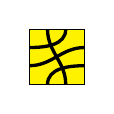
\begin{tikzpicture}[x=7mm,y=7mm]

\draw[black,fill=yellow] (0.000000,0.000000) rectangle (1.000000,-1.000000);
\draw[out=-90,in=90,looseness=1,very thick] (0.330000,0.000000) to (0.660000,-1.000000);
\draw[out=-90,in=0,looseness=1,very thick] (0.660000,0.000000) to (0.000000,-0.330000);
\draw[out=180,in=0,looseness=1,very thick] (1.000000,-0.330000) to (0.000000,-0.660000);
\draw[out=180,in=90,looseness=1,very thick] (1.000000,-0.660000) to (0.330000,-1.000000);
\end{tikzpicture}

\item Player 2 \textcolor{blue}{\LARGE$\bullet$} plays at row 6, col 4:
\begin{center}

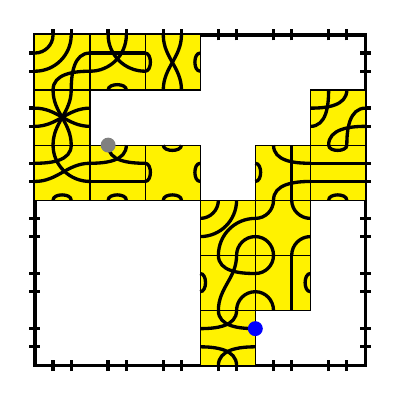
\begin{tikzpicture}[x=7mm,y=7mm]

\draw[very thick] (0.000000,0.000000) rectangle (6.000000,-6.000000);
\draw (0.000000,0.000000) grid[step=6] (6.000000,-6.000000);
\draw[very thick] (-0.100000,-0.330000) to (0.100000,-0.330000);
\draw[very thick] (5.900000,-0.330000) to (6.100000,-0.330000);
\draw[very thick] (0.330000,-0.100000) to (0.330000,0.100000);
\draw[very thick] (0.330000,-6.100000) to (0.330000,-5.900000);
\draw[very thick] (-0.100000,-0.660000) to (0.100000,-0.660000);
\draw[very thick] (5.900000,-0.660000) to (6.100000,-0.660000);
\draw[very thick] (0.660000,-0.100000) to (0.660000,0.100000);
\draw[very thick] (0.660000,-6.100000) to (0.660000,-5.900000);
\draw[very thick] (-0.100000,-1.330000) to (0.100000,-1.330000);
\draw[very thick] (5.900000,-1.330000) to (6.100000,-1.330000);
\draw[very thick] (1.330000,-0.100000) to (1.330000,0.100000);
\draw[very thick] (1.330000,-6.100000) to (1.330000,-5.900000);
\draw[very thick] (-0.100000,-1.660000) to (0.100000,-1.660000);
\draw[very thick] (5.900000,-1.660000) to (6.100000,-1.660000);
\draw[very thick] (1.660000,-0.100000) to (1.660000,0.100000);
\draw[very thick] (1.660000,-6.100000) to (1.660000,-5.900000);
\draw[very thick] (-0.100000,-2.330000) to (0.100000,-2.330000);
\draw[very thick] (5.900000,-2.330000) to (6.100000,-2.330000);
\draw[very thick] (2.330000,-0.100000) to (2.330000,0.100000);
\draw[very thick] (2.330000,-6.100000) to (2.330000,-5.900000);
\draw[very thick] (-0.100000,-2.660000) to (0.100000,-2.660000);
\draw[very thick] (5.900000,-2.660000) to (6.100000,-2.660000);
\draw[very thick] (2.660000,-0.100000) to (2.660000,0.100000);
\draw[very thick] (2.660000,-6.100000) to (2.660000,-5.900000);
\draw[very thick] (-0.100000,-3.330000) to (0.100000,-3.330000);
\draw[very thick] (5.900000,-3.330000) to (6.100000,-3.330000);
\draw[very thick] (3.330000,-0.100000) to (3.330000,0.100000);
\draw[very thick] (3.330000,-6.100000) to (3.330000,-5.900000);
\draw[very thick] (-0.100000,-3.660000) to (0.100000,-3.660000);
\draw[very thick] (5.900000,-3.660000) to (6.100000,-3.660000);
\draw[very thick] (3.660000,-0.100000) to (3.660000,0.100000);
\draw[very thick] (3.660000,-6.100000) to (3.660000,-5.900000);
\draw[very thick] (-0.100000,-4.330000) to (0.100000,-4.330000);
\draw[very thick] (5.900000,-4.330000) to (6.100000,-4.330000);
\draw[very thick] (4.330000,-0.100000) to (4.330000,0.100000);
\draw[very thick] (4.330000,-6.100000) to (4.330000,-5.900000);
\draw[very thick] (-0.100000,-4.660000) to (0.100000,-4.660000);
\draw[very thick] (5.900000,-4.660000) to (6.100000,-4.660000);
\draw[very thick] (4.660000,-0.100000) to (4.660000,0.100000);
\draw[very thick] (4.660000,-6.100000) to (4.660000,-5.900000);
\draw[very thick] (-0.100000,-5.330000) to (0.100000,-5.330000);
\draw[very thick] (5.900000,-5.330000) to (6.100000,-5.330000);
\draw[very thick] (5.330000,-0.100000) to (5.330000,0.100000);
\draw[very thick] (5.330000,-6.100000) to (5.330000,-5.900000);
\draw[very thick] (-0.100000,-5.660000) to (0.100000,-5.660000);
\draw[very thick] (5.900000,-5.660000) to (6.100000,-5.660000);
\draw[very thick] (5.660000,-0.100000) to (5.660000,0.100000);
\draw[very thick] (5.660000,-6.100000) to (5.660000,-5.900000);
\draw[black,fill=yellow] (0.000000,0.000000) rectangle (1.000000,-1.000000);
\draw[out=-90,in=0,looseness=1,very thick] (0.330000,0.000000) to (0.000000,-0.330000);
\draw[out=-90,in=0,looseness=1,very thick] (0.660000,0.000000) to (0.000000,-0.660000);
\draw[out=180,in=90,looseness=1,very thick] (1.000000,-0.330000) to (0.660000,-1.000000);
\draw[out=180,in=90,looseness=1,very thick] (1.000000,-0.660000) to (0.330000,-1.000000);
\draw[black,fill=yellow] (0.000000,-1.000000) rectangle (1.000000,-2.000000);
\draw[out=-90,in=90,looseness=1,very thick] (0.330000,-1.000000) to (0.660000,-2.000000);
\draw[out=-90,in=90,looseness=1,very thick] (0.660000,-1.000000) to (0.330000,-2.000000);
\draw[out=180,in=0,looseness=1,very thick] (1.000000,-1.330000) to (0.000000,-1.660000);
\draw[out=180,in=0,looseness=1,very thick] (1.000000,-1.660000) to (0.000000,-1.330000);
\draw[black,fill=yellow] (0.000000,-2.000000) rectangle (1.000000,-3.000000);
\draw[out=-90,in=180,looseness=1,very thick] (0.330000,-2.000000) to (1.000000,-2.660000);
\draw[out=-90,in=0,looseness=1,very thick] (0.660000,-2.000000) to (0.000000,-2.330000);
\draw[out=180,in=0,looseness=1,very thick] (1.000000,-2.330000) to (0.000000,-2.660000);
\draw[out=90,in=90,looseness=1,very thick] (0.660000,-3.000000) to (0.330000,-3.000000);
\draw[black,fill=yellow] (1.000000,0.000000) rectangle (2.000000,-1.000000);
\draw[out=-90,in=180,looseness=1,very thick] (1.330000,0.000000) to (2.000000,-0.660000);
\draw[out=-90,in=0,looseness=1,very thick] (1.660000,0.000000) to (1.000000,-0.660000);
\draw[out=180,in=0,looseness=1,very thick] (2.000000,-0.330000) to (1.000000,-0.330000);
\draw[out=90,in=90,looseness=1,very thick] (1.660000,-1.000000) to (1.330000,-1.000000);
\draw[black,fill=yellow] (1.000000,-2.000000) rectangle (2.000000,-3.000000);
\draw[out=-90,in=180,looseness=1,very thick] (1.330000,-2.000000) to (2.000000,-2.330000);
\draw[out=-90,in=0,looseness=1,very thick] (1.660000,-2.000000) to (1.000000,-2.330000);
\draw[out=180,in=0,looseness=1,very thick] (2.000000,-2.660000) to (1.000000,-2.660000);
\draw[out=90,in=90,looseness=1,very thick] (1.660000,-3.000000) to (1.330000,-3.000000);
\draw[black,fill=yellow] (2.000000,0.000000) rectangle (3.000000,-1.000000);
\draw[out=-90,in=90,looseness=1,very thick] (2.330000,0.000000) to (2.660000,-1.000000);
\draw[out=-90,in=90,looseness=1,very thick] (2.660000,0.000000) to (2.330000,-1.000000);
\draw[out=180,in=180,looseness=1,very thick] (3.000000,-0.330000) to (3.000000,-0.660000);
\draw[out=0,in=0,looseness=1,very thick] (2.000000,-0.660000) to (2.000000,-0.330000);
\draw[black,fill=yellow] (2.000000,-2.000000) rectangle (3.000000,-3.000000);
\draw[out=-90,in=-90,looseness=1,very thick] (2.330000,-2.000000) to (2.660000,-2.000000);
\draw[out=180,in=180,looseness=1,very thick] (3.000000,-2.330000) to (3.000000,-2.660000);
\draw[out=90,in=90,looseness=1,very thick] (2.660000,-3.000000) to (2.330000,-3.000000);
\draw[out=0,in=0,looseness=1,very thick] (2.000000,-2.660000) to (2.000000,-2.330000);
\draw[black,fill=yellow] (3.000000,-3.000000) rectangle (4.000000,-4.000000);
\draw[out=-90,in=0,looseness=1,very thick] (3.330000,-3.000000) to (3.000000,-3.330000);
\draw[out=-90,in=0,looseness=1,very thick] (3.660000,-3.000000) to (3.000000,-3.660000);
\draw[out=180,in=90,looseness=1,very thick] (4.000000,-3.330000) to (3.330000,-4.000000);
\draw[out=180,in=90,looseness=1,very thick] (4.000000,-3.660000) to (3.660000,-4.000000);
\draw[black,fill=yellow] (3.000000,-4.000000) rectangle (4.000000,-5.000000);
\draw[out=-90,in=180,looseness=1,very thick] (3.330000,-4.000000) to (4.000000,-4.330000);
\draw[out=-90,in=90,looseness=1,very thick] (3.660000,-4.000000) to (3.330000,-5.000000);
\draw[out=180,in=90,looseness=1,very thick] (4.000000,-4.660000) to (3.660000,-5.000000);
\draw[out=0,in=0,looseness=1,very thick] (3.000000,-4.660000) to (3.000000,-4.330000);
\draw[black,fill=yellow] (3.000000,-5.000000) rectangle (4.000000,-6.000000);
\draw[out=-90,in=180,looseness=1,very thick] (3.330000,-5.000000) to (4.000000,-5.330000);
\draw[out=-90,in=0,looseness=1,very thick] (3.660000,-5.000000) to (3.000000,-5.330000);
\draw[out=180,in=90,looseness=1,very thick] (4.000000,-5.660000) to (3.330000,-6.000000);
\draw[out=90,in=0,looseness=1,very thick] (3.660000,-6.000000) to (3.000000,-5.660000);
\draw[black,fill=yellow] (4.000000,-2.000000) rectangle (5.000000,-3.000000);
\draw[out=-90,in=180,looseness=1,very thick] (4.330000,-2.000000) to (5.000000,-2.330000);
\draw[out=-90,in=90,looseness=1,very thick] (4.660000,-2.000000) to (4.660000,-3.000000);
\draw[out=180,in=90,looseness=1,very thick] (5.000000,-2.660000) to (4.330000,-3.000000);
\draw[out=0,in=0,looseness=1,very thick] (4.000000,-2.660000) to (4.000000,-2.330000);
\draw[black,fill=yellow] (4.000000,-3.000000) rectangle (5.000000,-4.000000);
\draw[out=-90,in=0,looseness=1,very thick] (4.330000,-3.000000) to (4.000000,-3.330000);
\draw[out=-90,in=180,looseness=1,very thick] (4.660000,-3.000000) to (5.000000,-3.330000);
\draw[out=180,in=90,looseness=1,very thick] (5.000000,-3.660000) to (4.660000,-4.000000);
\draw[out=90,in=0,looseness=1,very thick] (4.330000,-4.000000) to (4.000000,-3.660000);
\draw[black,fill=yellow] (4.000000,-4.000000) rectangle (5.000000,-5.000000);
\draw[out=-90,in=0,looseness=1,very thick] (4.330000,-4.000000) to (4.000000,-4.330000);
\draw[out=-90,in=90,looseness=1,very thick] (4.660000,-4.000000) to (4.660000,-5.000000);
\draw[out=180,in=180,looseness=1,very thick] (5.000000,-4.330000) to (5.000000,-4.660000);
\draw[out=90,in=0,looseness=1,very thick] (4.330000,-5.000000) to (4.000000,-4.660000);
\draw[black,fill=yellow] (5.000000,-1.000000) rectangle (6.000000,-2.000000);
\draw[out=-90,in=0,looseness=1,very thick] (5.330000,-1.000000) to (5.000000,-1.660000);
\draw[out=-90,in=0,looseness=1,very thick] (5.660000,-1.000000) to (5.000000,-1.330000);
\draw[out=180,in=90,looseness=1,very thick] (6.000000,-1.330000) to (5.660000,-2.000000);
\draw[out=180,in=90,looseness=1,very thick] (6.000000,-1.660000) to (5.330000,-2.000000);
\draw[black,fill=yellow] (5.000000,-2.000000) rectangle (6.000000,-3.000000);
\draw[out=-90,in=-90,looseness=1,very thick] (5.330000,-2.000000) to (5.660000,-2.000000);
\draw[out=180,in=0,looseness=1,very thick] (6.000000,-2.330000) to (5.000000,-2.330000);
\draw[out=180,in=0,looseness=1,very thick] (6.000000,-2.660000) to (5.000000,-2.660000);
\draw[out=90,in=90,looseness=1,very thick] (5.660000,-3.000000) to (5.330000,-3.000000);
\draw[draw=blue,fill=blue] (4.000000,-5.330000) circle [x radius=0.125000,y radius=0.125000];
\draw[draw=gray,fill=gray] (1.330000,-2.000000) circle [x radius=0.125000,y radius=0.125000];
\end{tikzpicture}

\end{center}

\item[(27)] Player 2 \textcolor{blue}{\LARGE$\bullet$} draws 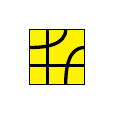
\begin{tikzpicture}[x=7mm,y=7mm]

\draw[black,fill=yellow] (0.000000,0.000000) rectangle (1.000000,-1.000000);
\draw[out=-90,in=90,looseness=1,very thick] (0.330000,0.000000) to (0.330000,-1.000000);
\draw[out=-90,in=0,looseness=1,very thick] (0.660000,0.000000) to (0.000000,-0.330000);
\draw[out=180,in=90,looseness=1,very thick] (1.000000,-0.330000) to (0.660000,-1.000000);
\draw[out=180,in=0,looseness=1,very thick] (1.000000,-0.660000) to (0.000000,-0.660000);
\end{tikzpicture}

\item Player 1 \textcolor{gray}{\LARGE$\bullet$} plays at row 2, col 2:
\begin{center}

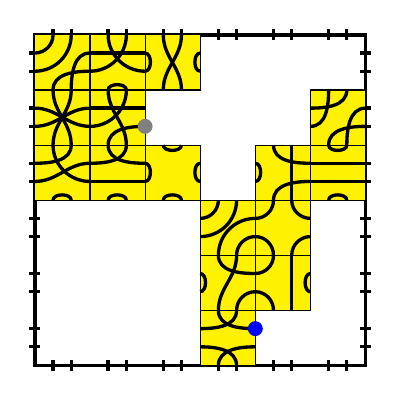
\begin{tikzpicture}[x=7mm,y=7mm]

\draw[very thick] (0.000000,0.000000) rectangle (6.000000,-6.000000);
\draw (0.000000,0.000000) grid[step=6] (6.000000,-6.000000);
\draw[very thick] (-0.100000,-0.330000) to (0.100000,-0.330000);
\draw[very thick] (5.900000,-0.330000) to (6.100000,-0.330000);
\draw[very thick] (0.330000,-0.100000) to (0.330000,0.100000);
\draw[very thick] (0.330000,-6.100000) to (0.330000,-5.900000);
\draw[very thick] (-0.100000,-0.660000) to (0.100000,-0.660000);
\draw[very thick] (5.900000,-0.660000) to (6.100000,-0.660000);
\draw[very thick] (0.660000,-0.100000) to (0.660000,0.100000);
\draw[very thick] (0.660000,-6.100000) to (0.660000,-5.900000);
\draw[very thick] (-0.100000,-1.330000) to (0.100000,-1.330000);
\draw[very thick] (5.900000,-1.330000) to (6.100000,-1.330000);
\draw[very thick] (1.330000,-0.100000) to (1.330000,0.100000);
\draw[very thick] (1.330000,-6.100000) to (1.330000,-5.900000);
\draw[very thick] (-0.100000,-1.660000) to (0.100000,-1.660000);
\draw[very thick] (5.900000,-1.660000) to (6.100000,-1.660000);
\draw[very thick] (1.660000,-0.100000) to (1.660000,0.100000);
\draw[very thick] (1.660000,-6.100000) to (1.660000,-5.900000);
\draw[very thick] (-0.100000,-2.330000) to (0.100000,-2.330000);
\draw[very thick] (5.900000,-2.330000) to (6.100000,-2.330000);
\draw[very thick] (2.330000,-0.100000) to (2.330000,0.100000);
\draw[very thick] (2.330000,-6.100000) to (2.330000,-5.900000);
\draw[very thick] (-0.100000,-2.660000) to (0.100000,-2.660000);
\draw[very thick] (5.900000,-2.660000) to (6.100000,-2.660000);
\draw[very thick] (2.660000,-0.100000) to (2.660000,0.100000);
\draw[very thick] (2.660000,-6.100000) to (2.660000,-5.900000);
\draw[very thick] (-0.100000,-3.330000) to (0.100000,-3.330000);
\draw[very thick] (5.900000,-3.330000) to (6.100000,-3.330000);
\draw[very thick] (3.330000,-0.100000) to (3.330000,0.100000);
\draw[very thick] (3.330000,-6.100000) to (3.330000,-5.900000);
\draw[very thick] (-0.100000,-3.660000) to (0.100000,-3.660000);
\draw[very thick] (5.900000,-3.660000) to (6.100000,-3.660000);
\draw[very thick] (3.660000,-0.100000) to (3.660000,0.100000);
\draw[very thick] (3.660000,-6.100000) to (3.660000,-5.900000);
\draw[very thick] (-0.100000,-4.330000) to (0.100000,-4.330000);
\draw[very thick] (5.900000,-4.330000) to (6.100000,-4.330000);
\draw[very thick] (4.330000,-0.100000) to (4.330000,0.100000);
\draw[very thick] (4.330000,-6.100000) to (4.330000,-5.900000);
\draw[very thick] (-0.100000,-4.660000) to (0.100000,-4.660000);
\draw[very thick] (5.900000,-4.660000) to (6.100000,-4.660000);
\draw[very thick] (4.660000,-0.100000) to (4.660000,0.100000);
\draw[very thick] (4.660000,-6.100000) to (4.660000,-5.900000);
\draw[very thick] (-0.100000,-5.330000) to (0.100000,-5.330000);
\draw[very thick] (5.900000,-5.330000) to (6.100000,-5.330000);
\draw[very thick] (5.330000,-0.100000) to (5.330000,0.100000);
\draw[very thick] (5.330000,-6.100000) to (5.330000,-5.900000);
\draw[very thick] (-0.100000,-5.660000) to (0.100000,-5.660000);
\draw[very thick] (5.900000,-5.660000) to (6.100000,-5.660000);
\draw[very thick] (5.660000,-0.100000) to (5.660000,0.100000);
\draw[very thick] (5.660000,-6.100000) to (5.660000,-5.900000);
\draw[black,fill=yellow] (0.000000,0.000000) rectangle (1.000000,-1.000000);
\draw[out=-90,in=0,looseness=1,very thick] (0.330000,0.000000) to (0.000000,-0.330000);
\draw[out=-90,in=0,looseness=1,very thick] (0.660000,0.000000) to (0.000000,-0.660000);
\draw[out=180,in=90,looseness=1,very thick] (1.000000,-0.330000) to (0.660000,-1.000000);
\draw[out=180,in=90,looseness=1,very thick] (1.000000,-0.660000) to (0.330000,-1.000000);
\draw[black,fill=yellow] (0.000000,-1.000000) rectangle (1.000000,-2.000000);
\draw[out=-90,in=90,looseness=1,very thick] (0.330000,-1.000000) to (0.660000,-2.000000);
\draw[out=-90,in=90,looseness=1,very thick] (0.660000,-1.000000) to (0.330000,-2.000000);
\draw[out=180,in=0,looseness=1,very thick] (1.000000,-1.330000) to (0.000000,-1.660000);
\draw[out=180,in=0,looseness=1,very thick] (1.000000,-1.660000) to (0.000000,-1.330000);
\draw[black,fill=yellow] (0.000000,-2.000000) rectangle (1.000000,-3.000000);
\draw[out=-90,in=180,looseness=1,very thick] (0.330000,-2.000000) to (1.000000,-2.660000);
\draw[out=-90,in=0,looseness=1,very thick] (0.660000,-2.000000) to (0.000000,-2.330000);
\draw[out=180,in=0,looseness=1,very thick] (1.000000,-2.330000) to (0.000000,-2.660000);
\draw[out=90,in=90,looseness=1,very thick] (0.660000,-3.000000) to (0.330000,-3.000000);
\draw[black,fill=yellow] (1.000000,0.000000) rectangle (2.000000,-1.000000);
\draw[out=-90,in=180,looseness=1,very thick] (1.330000,0.000000) to (2.000000,-0.660000);
\draw[out=-90,in=0,looseness=1,very thick] (1.660000,0.000000) to (1.000000,-0.660000);
\draw[out=180,in=0,looseness=1,very thick] (2.000000,-0.330000) to (1.000000,-0.330000);
\draw[out=90,in=90,looseness=1,very thick] (1.660000,-1.000000) to (1.330000,-1.000000);
\draw[black,fill=yellow] (1.000000,-1.000000) rectangle (2.000000,-2.000000);
\draw[out=-90,in=90,looseness=1,very thick] (1.330000,-1.000000) to (1.660000,-2.000000);
\draw[out=-90,in=0,looseness=1,very thick] (1.660000,-1.000000) to (1.000000,-1.660000);
\draw[out=180,in=0,looseness=1,very thick] (2.000000,-1.330000) to (1.000000,-1.330000);
\draw[out=180,in=90,looseness=1,very thick] (2.000000,-1.660000) to (1.330000,-2.000000);
\draw[black,fill=yellow] (1.000000,-2.000000) rectangle (2.000000,-3.000000);
\draw[out=-90,in=180,looseness=1,very thick] (1.330000,-2.000000) to (2.000000,-2.330000);
\draw[out=-90,in=0,looseness=1,very thick] (1.660000,-2.000000) to (1.000000,-2.330000);
\draw[out=180,in=0,looseness=1,very thick] (2.000000,-2.660000) to (1.000000,-2.660000);
\draw[out=90,in=90,looseness=1,very thick] (1.660000,-3.000000) to (1.330000,-3.000000);
\draw[black,fill=yellow] (2.000000,0.000000) rectangle (3.000000,-1.000000);
\draw[out=-90,in=90,looseness=1,very thick] (2.330000,0.000000) to (2.660000,-1.000000);
\draw[out=-90,in=90,looseness=1,very thick] (2.660000,0.000000) to (2.330000,-1.000000);
\draw[out=180,in=180,looseness=1,very thick] (3.000000,-0.330000) to (3.000000,-0.660000);
\draw[out=0,in=0,looseness=1,very thick] (2.000000,-0.660000) to (2.000000,-0.330000);
\draw[black,fill=yellow] (2.000000,-2.000000) rectangle (3.000000,-3.000000);
\draw[out=-90,in=-90,looseness=1,very thick] (2.330000,-2.000000) to (2.660000,-2.000000);
\draw[out=180,in=180,looseness=1,very thick] (3.000000,-2.330000) to (3.000000,-2.660000);
\draw[out=90,in=90,looseness=1,very thick] (2.660000,-3.000000) to (2.330000,-3.000000);
\draw[out=0,in=0,looseness=1,very thick] (2.000000,-2.660000) to (2.000000,-2.330000);
\draw[black,fill=yellow] (3.000000,-3.000000) rectangle (4.000000,-4.000000);
\draw[out=-90,in=0,looseness=1,very thick] (3.330000,-3.000000) to (3.000000,-3.330000);
\draw[out=-90,in=0,looseness=1,very thick] (3.660000,-3.000000) to (3.000000,-3.660000);
\draw[out=180,in=90,looseness=1,very thick] (4.000000,-3.330000) to (3.330000,-4.000000);
\draw[out=180,in=90,looseness=1,very thick] (4.000000,-3.660000) to (3.660000,-4.000000);
\draw[black,fill=yellow] (3.000000,-4.000000) rectangle (4.000000,-5.000000);
\draw[out=-90,in=180,looseness=1,very thick] (3.330000,-4.000000) to (4.000000,-4.330000);
\draw[out=-90,in=90,looseness=1,very thick] (3.660000,-4.000000) to (3.330000,-5.000000);
\draw[out=180,in=90,looseness=1,very thick] (4.000000,-4.660000) to (3.660000,-5.000000);
\draw[out=0,in=0,looseness=1,very thick] (3.000000,-4.660000) to (3.000000,-4.330000);
\draw[black,fill=yellow] (3.000000,-5.000000) rectangle (4.000000,-6.000000);
\draw[out=-90,in=180,looseness=1,very thick] (3.330000,-5.000000) to (4.000000,-5.330000);
\draw[out=-90,in=0,looseness=1,very thick] (3.660000,-5.000000) to (3.000000,-5.330000);
\draw[out=180,in=90,looseness=1,very thick] (4.000000,-5.660000) to (3.330000,-6.000000);
\draw[out=90,in=0,looseness=1,very thick] (3.660000,-6.000000) to (3.000000,-5.660000);
\draw[black,fill=yellow] (4.000000,-2.000000) rectangle (5.000000,-3.000000);
\draw[out=-90,in=180,looseness=1,very thick] (4.330000,-2.000000) to (5.000000,-2.330000);
\draw[out=-90,in=90,looseness=1,very thick] (4.660000,-2.000000) to (4.660000,-3.000000);
\draw[out=180,in=90,looseness=1,very thick] (5.000000,-2.660000) to (4.330000,-3.000000);
\draw[out=0,in=0,looseness=1,very thick] (4.000000,-2.660000) to (4.000000,-2.330000);
\draw[black,fill=yellow] (4.000000,-3.000000) rectangle (5.000000,-4.000000);
\draw[out=-90,in=0,looseness=1,very thick] (4.330000,-3.000000) to (4.000000,-3.330000);
\draw[out=-90,in=180,looseness=1,very thick] (4.660000,-3.000000) to (5.000000,-3.330000);
\draw[out=180,in=90,looseness=1,very thick] (5.000000,-3.660000) to (4.660000,-4.000000);
\draw[out=90,in=0,looseness=1,very thick] (4.330000,-4.000000) to (4.000000,-3.660000);
\draw[black,fill=yellow] (4.000000,-4.000000) rectangle (5.000000,-5.000000);
\draw[out=-90,in=0,looseness=1,very thick] (4.330000,-4.000000) to (4.000000,-4.330000);
\draw[out=-90,in=90,looseness=1,very thick] (4.660000,-4.000000) to (4.660000,-5.000000);
\draw[out=180,in=180,looseness=1,very thick] (5.000000,-4.330000) to (5.000000,-4.660000);
\draw[out=90,in=0,looseness=1,very thick] (4.330000,-5.000000) to (4.000000,-4.660000);
\draw[black,fill=yellow] (5.000000,-1.000000) rectangle (6.000000,-2.000000);
\draw[out=-90,in=0,looseness=1,very thick] (5.330000,-1.000000) to (5.000000,-1.660000);
\draw[out=-90,in=0,looseness=1,very thick] (5.660000,-1.000000) to (5.000000,-1.330000);
\draw[out=180,in=90,looseness=1,very thick] (6.000000,-1.330000) to (5.660000,-2.000000);
\draw[out=180,in=90,looseness=1,very thick] (6.000000,-1.660000) to (5.330000,-2.000000);
\draw[black,fill=yellow] (5.000000,-2.000000) rectangle (6.000000,-3.000000);
\draw[out=-90,in=-90,looseness=1,very thick] (5.330000,-2.000000) to (5.660000,-2.000000);
\draw[out=180,in=0,looseness=1,very thick] (6.000000,-2.330000) to (5.000000,-2.330000);
\draw[out=180,in=0,looseness=1,very thick] (6.000000,-2.660000) to (5.000000,-2.660000);
\draw[out=90,in=90,looseness=1,very thick] (5.660000,-3.000000) to (5.330000,-3.000000);
\draw[draw=blue,fill=blue] (4.000000,-5.330000) circle [x radius=0.125000,y radius=0.125000];
\draw[draw=gray,fill=gray] (2.000000,-1.660000) circle [x radius=0.125000,y radius=0.125000];
\end{tikzpicture}

\end{center}

\item[(28)] Player 1 \textcolor{gray}{\LARGE$\bullet$} draws 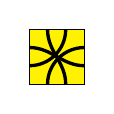
\begin{tikzpicture}[x=7mm,y=7mm]

\draw[black,fill=yellow] (0.000000,0.000000) rectangle (1.000000,-1.000000);
\draw[out=-90,in=90,looseness=1,very thick] (0.330000,0.000000) to (0.660000,-1.000000);
\draw[out=-90,in=0,looseness=1,very thick] (0.660000,0.000000) to (0.000000,-0.660000);
\draw[out=180,in=90,looseness=1,very thick] (1.000000,-0.330000) to (0.330000,-1.000000);
\draw[out=180,in=0,looseness=1,very thick] (1.000000,-0.660000) to (0.000000,-0.330000);
\end{tikzpicture}

\item Player 2 \textcolor{blue}{\LARGE$\bullet$} plays at row 6, col 5:
\begin{center}

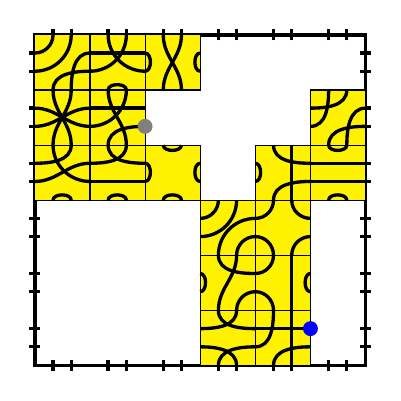
\begin{tikzpicture}[x=7mm,y=7mm]

\draw[very thick] (0.000000,0.000000) rectangle (6.000000,-6.000000);
\draw (0.000000,0.000000) grid[step=6] (6.000000,-6.000000);
\draw[very thick] (-0.100000,-0.330000) to (0.100000,-0.330000);
\draw[very thick] (5.900000,-0.330000) to (6.100000,-0.330000);
\draw[very thick] (0.330000,-0.100000) to (0.330000,0.100000);
\draw[very thick] (0.330000,-6.100000) to (0.330000,-5.900000);
\draw[very thick] (-0.100000,-0.660000) to (0.100000,-0.660000);
\draw[very thick] (5.900000,-0.660000) to (6.100000,-0.660000);
\draw[very thick] (0.660000,-0.100000) to (0.660000,0.100000);
\draw[very thick] (0.660000,-6.100000) to (0.660000,-5.900000);
\draw[very thick] (-0.100000,-1.330000) to (0.100000,-1.330000);
\draw[very thick] (5.900000,-1.330000) to (6.100000,-1.330000);
\draw[very thick] (1.330000,-0.100000) to (1.330000,0.100000);
\draw[very thick] (1.330000,-6.100000) to (1.330000,-5.900000);
\draw[very thick] (-0.100000,-1.660000) to (0.100000,-1.660000);
\draw[very thick] (5.900000,-1.660000) to (6.100000,-1.660000);
\draw[very thick] (1.660000,-0.100000) to (1.660000,0.100000);
\draw[very thick] (1.660000,-6.100000) to (1.660000,-5.900000);
\draw[very thick] (-0.100000,-2.330000) to (0.100000,-2.330000);
\draw[very thick] (5.900000,-2.330000) to (6.100000,-2.330000);
\draw[very thick] (2.330000,-0.100000) to (2.330000,0.100000);
\draw[very thick] (2.330000,-6.100000) to (2.330000,-5.900000);
\draw[very thick] (-0.100000,-2.660000) to (0.100000,-2.660000);
\draw[very thick] (5.900000,-2.660000) to (6.100000,-2.660000);
\draw[very thick] (2.660000,-0.100000) to (2.660000,0.100000);
\draw[very thick] (2.660000,-6.100000) to (2.660000,-5.900000);
\draw[very thick] (-0.100000,-3.330000) to (0.100000,-3.330000);
\draw[very thick] (5.900000,-3.330000) to (6.100000,-3.330000);
\draw[very thick] (3.330000,-0.100000) to (3.330000,0.100000);
\draw[very thick] (3.330000,-6.100000) to (3.330000,-5.900000);
\draw[very thick] (-0.100000,-3.660000) to (0.100000,-3.660000);
\draw[very thick] (5.900000,-3.660000) to (6.100000,-3.660000);
\draw[very thick] (3.660000,-0.100000) to (3.660000,0.100000);
\draw[very thick] (3.660000,-6.100000) to (3.660000,-5.900000);
\draw[very thick] (-0.100000,-4.330000) to (0.100000,-4.330000);
\draw[very thick] (5.900000,-4.330000) to (6.100000,-4.330000);
\draw[very thick] (4.330000,-0.100000) to (4.330000,0.100000);
\draw[very thick] (4.330000,-6.100000) to (4.330000,-5.900000);
\draw[very thick] (-0.100000,-4.660000) to (0.100000,-4.660000);
\draw[very thick] (5.900000,-4.660000) to (6.100000,-4.660000);
\draw[very thick] (4.660000,-0.100000) to (4.660000,0.100000);
\draw[very thick] (4.660000,-6.100000) to (4.660000,-5.900000);
\draw[very thick] (-0.100000,-5.330000) to (0.100000,-5.330000);
\draw[very thick] (5.900000,-5.330000) to (6.100000,-5.330000);
\draw[very thick] (5.330000,-0.100000) to (5.330000,0.100000);
\draw[very thick] (5.330000,-6.100000) to (5.330000,-5.900000);
\draw[very thick] (-0.100000,-5.660000) to (0.100000,-5.660000);
\draw[very thick] (5.900000,-5.660000) to (6.100000,-5.660000);
\draw[very thick] (5.660000,-0.100000) to (5.660000,0.100000);
\draw[very thick] (5.660000,-6.100000) to (5.660000,-5.900000);
\draw[black,fill=yellow] (0.000000,0.000000) rectangle (1.000000,-1.000000);
\draw[out=-90,in=0,looseness=1,very thick] (0.330000,0.000000) to (0.000000,-0.330000);
\draw[out=-90,in=0,looseness=1,very thick] (0.660000,0.000000) to (0.000000,-0.660000);
\draw[out=180,in=90,looseness=1,very thick] (1.000000,-0.330000) to (0.660000,-1.000000);
\draw[out=180,in=90,looseness=1,very thick] (1.000000,-0.660000) to (0.330000,-1.000000);
\draw[black,fill=yellow] (0.000000,-1.000000) rectangle (1.000000,-2.000000);
\draw[out=-90,in=90,looseness=1,very thick] (0.330000,-1.000000) to (0.660000,-2.000000);
\draw[out=-90,in=90,looseness=1,very thick] (0.660000,-1.000000) to (0.330000,-2.000000);
\draw[out=180,in=0,looseness=1,very thick] (1.000000,-1.330000) to (0.000000,-1.660000);
\draw[out=180,in=0,looseness=1,very thick] (1.000000,-1.660000) to (0.000000,-1.330000);
\draw[black,fill=yellow] (0.000000,-2.000000) rectangle (1.000000,-3.000000);
\draw[out=-90,in=180,looseness=1,very thick] (0.330000,-2.000000) to (1.000000,-2.660000);
\draw[out=-90,in=0,looseness=1,very thick] (0.660000,-2.000000) to (0.000000,-2.330000);
\draw[out=180,in=0,looseness=1,very thick] (1.000000,-2.330000) to (0.000000,-2.660000);
\draw[out=90,in=90,looseness=1,very thick] (0.660000,-3.000000) to (0.330000,-3.000000);
\draw[black,fill=yellow] (1.000000,0.000000) rectangle (2.000000,-1.000000);
\draw[out=-90,in=180,looseness=1,very thick] (1.330000,0.000000) to (2.000000,-0.660000);
\draw[out=-90,in=0,looseness=1,very thick] (1.660000,0.000000) to (1.000000,-0.660000);
\draw[out=180,in=0,looseness=1,very thick] (2.000000,-0.330000) to (1.000000,-0.330000);
\draw[out=90,in=90,looseness=1,very thick] (1.660000,-1.000000) to (1.330000,-1.000000);
\draw[black,fill=yellow] (1.000000,-1.000000) rectangle (2.000000,-2.000000);
\draw[out=-90,in=90,looseness=1,very thick] (1.330000,-1.000000) to (1.660000,-2.000000);
\draw[out=-90,in=0,looseness=1,very thick] (1.660000,-1.000000) to (1.000000,-1.660000);
\draw[out=180,in=0,looseness=1,very thick] (2.000000,-1.330000) to (1.000000,-1.330000);
\draw[out=180,in=90,looseness=1,very thick] (2.000000,-1.660000) to (1.330000,-2.000000);
\draw[black,fill=yellow] (1.000000,-2.000000) rectangle (2.000000,-3.000000);
\draw[out=-90,in=180,looseness=1,very thick] (1.330000,-2.000000) to (2.000000,-2.330000);
\draw[out=-90,in=0,looseness=1,very thick] (1.660000,-2.000000) to (1.000000,-2.330000);
\draw[out=180,in=0,looseness=1,very thick] (2.000000,-2.660000) to (1.000000,-2.660000);
\draw[out=90,in=90,looseness=1,very thick] (1.660000,-3.000000) to (1.330000,-3.000000);
\draw[black,fill=yellow] (2.000000,0.000000) rectangle (3.000000,-1.000000);
\draw[out=-90,in=90,looseness=1,very thick] (2.330000,0.000000) to (2.660000,-1.000000);
\draw[out=-90,in=90,looseness=1,very thick] (2.660000,0.000000) to (2.330000,-1.000000);
\draw[out=180,in=180,looseness=1,very thick] (3.000000,-0.330000) to (3.000000,-0.660000);
\draw[out=0,in=0,looseness=1,very thick] (2.000000,-0.660000) to (2.000000,-0.330000);
\draw[black,fill=yellow] (2.000000,-2.000000) rectangle (3.000000,-3.000000);
\draw[out=-90,in=-90,looseness=1,very thick] (2.330000,-2.000000) to (2.660000,-2.000000);
\draw[out=180,in=180,looseness=1,very thick] (3.000000,-2.330000) to (3.000000,-2.660000);
\draw[out=90,in=90,looseness=1,very thick] (2.660000,-3.000000) to (2.330000,-3.000000);
\draw[out=0,in=0,looseness=1,very thick] (2.000000,-2.660000) to (2.000000,-2.330000);
\draw[black,fill=yellow] (3.000000,-3.000000) rectangle (4.000000,-4.000000);
\draw[out=-90,in=0,looseness=1,very thick] (3.330000,-3.000000) to (3.000000,-3.330000);
\draw[out=-90,in=0,looseness=1,very thick] (3.660000,-3.000000) to (3.000000,-3.660000);
\draw[out=180,in=90,looseness=1,very thick] (4.000000,-3.330000) to (3.330000,-4.000000);
\draw[out=180,in=90,looseness=1,very thick] (4.000000,-3.660000) to (3.660000,-4.000000);
\draw[black,fill=yellow] (3.000000,-4.000000) rectangle (4.000000,-5.000000);
\draw[out=-90,in=180,looseness=1,very thick] (3.330000,-4.000000) to (4.000000,-4.330000);
\draw[out=-90,in=90,looseness=1,very thick] (3.660000,-4.000000) to (3.330000,-5.000000);
\draw[out=180,in=90,looseness=1,very thick] (4.000000,-4.660000) to (3.660000,-5.000000);
\draw[out=0,in=0,looseness=1,very thick] (3.000000,-4.660000) to (3.000000,-4.330000);
\draw[black,fill=yellow] (3.000000,-5.000000) rectangle (4.000000,-6.000000);
\draw[out=-90,in=180,looseness=1,very thick] (3.330000,-5.000000) to (4.000000,-5.330000);
\draw[out=-90,in=0,looseness=1,very thick] (3.660000,-5.000000) to (3.000000,-5.330000);
\draw[out=180,in=90,looseness=1,very thick] (4.000000,-5.660000) to (3.330000,-6.000000);
\draw[out=90,in=0,looseness=1,very thick] (3.660000,-6.000000) to (3.000000,-5.660000);
\draw[black,fill=yellow] (4.000000,-2.000000) rectangle (5.000000,-3.000000);
\draw[out=-90,in=180,looseness=1,very thick] (4.330000,-2.000000) to (5.000000,-2.330000);
\draw[out=-90,in=90,looseness=1,very thick] (4.660000,-2.000000) to (4.660000,-3.000000);
\draw[out=180,in=90,looseness=1,very thick] (5.000000,-2.660000) to (4.330000,-3.000000);
\draw[out=0,in=0,looseness=1,very thick] (4.000000,-2.660000) to (4.000000,-2.330000);
\draw[black,fill=yellow] (4.000000,-3.000000) rectangle (5.000000,-4.000000);
\draw[out=-90,in=0,looseness=1,very thick] (4.330000,-3.000000) to (4.000000,-3.330000);
\draw[out=-90,in=180,looseness=1,very thick] (4.660000,-3.000000) to (5.000000,-3.330000);
\draw[out=180,in=90,looseness=1,very thick] (5.000000,-3.660000) to (4.660000,-4.000000);
\draw[out=90,in=0,looseness=1,very thick] (4.330000,-4.000000) to (4.000000,-3.660000);
\draw[black,fill=yellow] (4.000000,-4.000000) rectangle (5.000000,-5.000000);
\draw[out=-90,in=0,looseness=1,very thick] (4.330000,-4.000000) to (4.000000,-4.330000);
\draw[out=-90,in=90,looseness=1,very thick] (4.660000,-4.000000) to (4.660000,-5.000000);
\draw[out=180,in=180,looseness=1,very thick] (5.000000,-4.330000) to (5.000000,-4.660000);
\draw[out=90,in=0,looseness=1,very thick] (4.330000,-5.000000) to (4.000000,-4.660000);
\draw[black,fill=yellow] (4.000000,-5.000000) rectangle (5.000000,-6.000000);
\draw[out=-90,in=0,looseness=1,very thick] (4.330000,-5.000000) to (4.000000,-5.660000);
\draw[out=-90,in=90,looseness=1,very thick] (4.660000,-5.000000) to (4.660000,-6.000000);
\draw[out=180,in=0,looseness=1,very thick] (5.000000,-5.330000) to (4.000000,-5.330000);
\draw[out=180,in=90,looseness=1,very thick] (5.000000,-5.660000) to (4.330000,-6.000000);
\draw[black,fill=yellow] (5.000000,-1.000000) rectangle (6.000000,-2.000000);
\draw[out=-90,in=0,looseness=1,very thick] (5.330000,-1.000000) to (5.000000,-1.660000);
\draw[out=-90,in=0,looseness=1,very thick] (5.660000,-1.000000) to (5.000000,-1.330000);
\draw[out=180,in=90,looseness=1,very thick] (6.000000,-1.330000) to (5.660000,-2.000000);
\draw[out=180,in=90,looseness=1,very thick] (6.000000,-1.660000) to (5.330000,-2.000000);
\draw[black,fill=yellow] (5.000000,-2.000000) rectangle (6.000000,-3.000000);
\draw[out=-90,in=-90,looseness=1,very thick] (5.330000,-2.000000) to (5.660000,-2.000000);
\draw[out=180,in=0,looseness=1,very thick] (6.000000,-2.330000) to (5.000000,-2.330000);
\draw[out=180,in=0,looseness=1,very thick] (6.000000,-2.660000) to (5.000000,-2.660000);
\draw[out=90,in=90,looseness=1,very thick] (5.660000,-3.000000) to (5.330000,-3.000000);
\draw[draw=blue,fill=blue] (5.000000,-5.330000) circle [x radius=0.125000,y radius=0.125000];
\draw[draw=gray,fill=gray] (2.000000,-1.660000) circle [x radius=0.125000,y radius=0.125000];
\end{tikzpicture}

\end{center}

\item[(29)] Player 2 \textcolor{blue}{\LARGE$\bullet$} draws 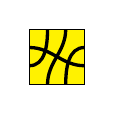
\begin{tikzpicture}[x=7mm,y=7mm]

\draw[black,fill=yellow] (0.000000,0.000000) rectangle (1.000000,-1.000000);
\draw[out=-90,in=0,looseness=1,very thick] (0.330000,0.000000) to (0.000000,-0.660000);
\draw[out=-90,in=90,looseness=1,very thick] (0.660000,0.000000) to (0.330000,-1.000000);
\draw[out=180,in=90,looseness=1,very thick] (1.000000,-0.330000) to (0.660000,-1.000000);
\draw[out=180,in=0,looseness=1,very thick] (1.000000,-0.660000) to (0.000000,-0.330000);
\end{tikzpicture}

\item Player 1 \textcolor{gray}{\LARGE$\bullet$} plays at row 2, col 3:
\begin{center}

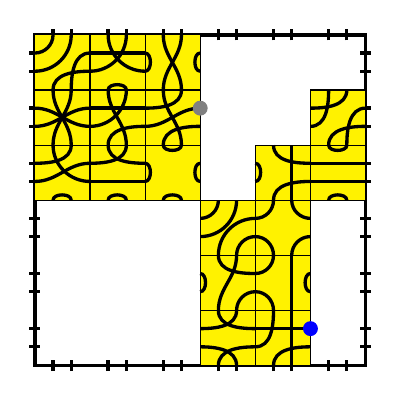
\begin{tikzpicture}[x=7mm,y=7mm]

\draw[very thick] (0.000000,0.000000) rectangle (6.000000,-6.000000);
\draw (0.000000,0.000000) grid[step=6] (6.000000,-6.000000);
\draw[very thick] (-0.100000,-0.330000) to (0.100000,-0.330000);
\draw[very thick] (5.900000,-0.330000) to (6.100000,-0.330000);
\draw[very thick] (0.330000,-0.100000) to (0.330000,0.100000);
\draw[very thick] (0.330000,-6.100000) to (0.330000,-5.900000);
\draw[very thick] (-0.100000,-0.660000) to (0.100000,-0.660000);
\draw[very thick] (5.900000,-0.660000) to (6.100000,-0.660000);
\draw[very thick] (0.660000,-0.100000) to (0.660000,0.100000);
\draw[very thick] (0.660000,-6.100000) to (0.660000,-5.900000);
\draw[very thick] (-0.100000,-1.330000) to (0.100000,-1.330000);
\draw[very thick] (5.900000,-1.330000) to (6.100000,-1.330000);
\draw[very thick] (1.330000,-0.100000) to (1.330000,0.100000);
\draw[very thick] (1.330000,-6.100000) to (1.330000,-5.900000);
\draw[very thick] (-0.100000,-1.660000) to (0.100000,-1.660000);
\draw[very thick] (5.900000,-1.660000) to (6.100000,-1.660000);
\draw[very thick] (1.660000,-0.100000) to (1.660000,0.100000);
\draw[very thick] (1.660000,-6.100000) to (1.660000,-5.900000);
\draw[very thick] (-0.100000,-2.330000) to (0.100000,-2.330000);
\draw[very thick] (5.900000,-2.330000) to (6.100000,-2.330000);
\draw[very thick] (2.330000,-0.100000) to (2.330000,0.100000);
\draw[very thick] (2.330000,-6.100000) to (2.330000,-5.900000);
\draw[very thick] (-0.100000,-2.660000) to (0.100000,-2.660000);
\draw[very thick] (5.900000,-2.660000) to (6.100000,-2.660000);
\draw[very thick] (2.660000,-0.100000) to (2.660000,0.100000);
\draw[very thick] (2.660000,-6.100000) to (2.660000,-5.900000);
\draw[very thick] (-0.100000,-3.330000) to (0.100000,-3.330000);
\draw[very thick] (5.900000,-3.330000) to (6.100000,-3.330000);
\draw[very thick] (3.330000,-0.100000) to (3.330000,0.100000);
\draw[very thick] (3.330000,-6.100000) to (3.330000,-5.900000);
\draw[very thick] (-0.100000,-3.660000) to (0.100000,-3.660000);
\draw[very thick] (5.900000,-3.660000) to (6.100000,-3.660000);
\draw[very thick] (3.660000,-0.100000) to (3.660000,0.100000);
\draw[very thick] (3.660000,-6.100000) to (3.660000,-5.900000);
\draw[very thick] (-0.100000,-4.330000) to (0.100000,-4.330000);
\draw[very thick] (5.900000,-4.330000) to (6.100000,-4.330000);
\draw[very thick] (4.330000,-0.100000) to (4.330000,0.100000);
\draw[very thick] (4.330000,-6.100000) to (4.330000,-5.900000);
\draw[very thick] (-0.100000,-4.660000) to (0.100000,-4.660000);
\draw[very thick] (5.900000,-4.660000) to (6.100000,-4.660000);
\draw[very thick] (4.660000,-0.100000) to (4.660000,0.100000);
\draw[very thick] (4.660000,-6.100000) to (4.660000,-5.900000);
\draw[very thick] (-0.100000,-5.330000) to (0.100000,-5.330000);
\draw[very thick] (5.900000,-5.330000) to (6.100000,-5.330000);
\draw[very thick] (5.330000,-0.100000) to (5.330000,0.100000);
\draw[very thick] (5.330000,-6.100000) to (5.330000,-5.900000);
\draw[very thick] (-0.100000,-5.660000) to (0.100000,-5.660000);
\draw[very thick] (5.900000,-5.660000) to (6.100000,-5.660000);
\draw[very thick] (5.660000,-0.100000) to (5.660000,0.100000);
\draw[very thick] (5.660000,-6.100000) to (5.660000,-5.900000);
\draw[black,fill=yellow] (0.000000,0.000000) rectangle (1.000000,-1.000000);
\draw[out=-90,in=0,looseness=1,very thick] (0.330000,0.000000) to (0.000000,-0.330000);
\draw[out=-90,in=0,looseness=1,very thick] (0.660000,0.000000) to (0.000000,-0.660000);
\draw[out=180,in=90,looseness=1,very thick] (1.000000,-0.330000) to (0.660000,-1.000000);
\draw[out=180,in=90,looseness=1,very thick] (1.000000,-0.660000) to (0.330000,-1.000000);
\draw[black,fill=yellow] (0.000000,-1.000000) rectangle (1.000000,-2.000000);
\draw[out=-90,in=90,looseness=1,very thick] (0.330000,-1.000000) to (0.660000,-2.000000);
\draw[out=-90,in=90,looseness=1,very thick] (0.660000,-1.000000) to (0.330000,-2.000000);
\draw[out=180,in=0,looseness=1,very thick] (1.000000,-1.330000) to (0.000000,-1.660000);
\draw[out=180,in=0,looseness=1,very thick] (1.000000,-1.660000) to (0.000000,-1.330000);
\draw[black,fill=yellow] (0.000000,-2.000000) rectangle (1.000000,-3.000000);
\draw[out=-90,in=180,looseness=1,very thick] (0.330000,-2.000000) to (1.000000,-2.660000);
\draw[out=-90,in=0,looseness=1,very thick] (0.660000,-2.000000) to (0.000000,-2.330000);
\draw[out=180,in=0,looseness=1,very thick] (1.000000,-2.330000) to (0.000000,-2.660000);
\draw[out=90,in=90,looseness=1,very thick] (0.660000,-3.000000) to (0.330000,-3.000000);
\draw[black,fill=yellow] (1.000000,0.000000) rectangle (2.000000,-1.000000);
\draw[out=-90,in=180,looseness=1,very thick] (1.330000,0.000000) to (2.000000,-0.660000);
\draw[out=-90,in=0,looseness=1,very thick] (1.660000,0.000000) to (1.000000,-0.660000);
\draw[out=180,in=0,looseness=1,very thick] (2.000000,-0.330000) to (1.000000,-0.330000);
\draw[out=90,in=90,looseness=1,very thick] (1.660000,-1.000000) to (1.330000,-1.000000);
\draw[black,fill=yellow] (1.000000,-1.000000) rectangle (2.000000,-2.000000);
\draw[out=-90,in=90,looseness=1,very thick] (1.330000,-1.000000) to (1.660000,-2.000000);
\draw[out=-90,in=0,looseness=1,very thick] (1.660000,-1.000000) to (1.000000,-1.660000);
\draw[out=180,in=0,looseness=1,very thick] (2.000000,-1.330000) to (1.000000,-1.330000);
\draw[out=180,in=90,looseness=1,very thick] (2.000000,-1.660000) to (1.330000,-2.000000);
\draw[black,fill=yellow] (1.000000,-2.000000) rectangle (2.000000,-3.000000);
\draw[out=-90,in=180,looseness=1,very thick] (1.330000,-2.000000) to (2.000000,-2.330000);
\draw[out=-90,in=0,looseness=1,very thick] (1.660000,-2.000000) to (1.000000,-2.330000);
\draw[out=180,in=0,looseness=1,very thick] (2.000000,-2.660000) to (1.000000,-2.660000);
\draw[out=90,in=90,looseness=1,very thick] (1.660000,-3.000000) to (1.330000,-3.000000);
\draw[black,fill=yellow] (2.000000,0.000000) rectangle (3.000000,-1.000000);
\draw[out=-90,in=90,looseness=1,very thick] (2.330000,0.000000) to (2.660000,-1.000000);
\draw[out=-90,in=90,looseness=1,very thick] (2.660000,0.000000) to (2.330000,-1.000000);
\draw[out=180,in=180,looseness=1,very thick] (3.000000,-0.330000) to (3.000000,-0.660000);
\draw[out=0,in=0,looseness=1,very thick] (2.000000,-0.660000) to (2.000000,-0.330000);
\draw[black,fill=yellow] (2.000000,-1.000000) rectangle (3.000000,-2.000000);
\draw[out=-90,in=90,looseness=1,very thick] (2.330000,-1.000000) to (2.660000,-2.000000);
\draw[out=-90,in=0,looseness=1,very thick] (2.660000,-1.000000) to (2.000000,-1.330000);
\draw[out=180,in=0,looseness=1,very thick] (3.000000,-1.330000) to (2.000000,-1.660000);
\draw[out=180,in=90,looseness=1,very thick] (3.000000,-1.660000) to (2.330000,-2.000000);
\draw[black,fill=yellow] (2.000000,-2.000000) rectangle (3.000000,-3.000000);
\draw[out=-90,in=-90,looseness=1,very thick] (2.330000,-2.000000) to (2.660000,-2.000000);
\draw[out=180,in=180,looseness=1,very thick] (3.000000,-2.330000) to (3.000000,-2.660000);
\draw[out=90,in=90,looseness=1,very thick] (2.660000,-3.000000) to (2.330000,-3.000000);
\draw[out=0,in=0,looseness=1,very thick] (2.000000,-2.660000) to (2.000000,-2.330000);
\draw[black,fill=yellow] (3.000000,-3.000000) rectangle (4.000000,-4.000000);
\draw[out=-90,in=0,looseness=1,very thick] (3.330000,-3.000000) to (3.000000,-3.330000);
\draw[out=-90,in=0,looseness=1,very thick] (3.660000,-3.000000) to (3.000000,-3.660000);
\draw[out=180,in=90,looseness=1,very thick] (4.000000,-3.330000) to (3.330000,-4.000000);
\draw[out=180,in=90,looseness=1,very thick] (4.000000,-3.660000) to (3.660000,-4.000000);
\draw[black,fill=yellow] (3.000000,-4.000000) rectangle (4.000000,-5.000000);
\draw[out=-90,in=180,looseness=1,very thick] (3.330000,-4.000000) to (4.000000,-4.330000);
\draw[out=-90,in=90,looseness=1,very thick] (3.660000,-4.000000) to (3.330000,-5.000000);
\draw[out=180,in=90,looseness=1,very thick] (4.000000,-4.660000) to (3.660000,-5.000000);
\draw[out=0,in=0,looseness=1,very thick] (3.000000,-4.660000) to (3.000000,-4.330000);
\draw[black,fill=yellow] (3.000000,-5.000000) rectangle (4.000000,-6.000000);
\draw[out=-90,in=180,looseness=1,very thick] (3.330000,-5.000000) to (4.000000,-5.330000);
\draw[out=-90,in=0,looseness=1,very thick] (3.660000,-5.000000) to (3.000000,-5.330000);
\draw[out=180,in=90,looseness=1,very thick] (4.000000,-5.660000) to (3.330000,-6.000000);
\draw[out=90,in=0,looseness=1,very thick] (3.660000,-6.000000) to (3.000000,-5.660000);
\draw[black,fill=yellow] (4.000000,-2.000000) rectangle (5.000000,-3.000000);
\draw[out=-90,in=180,looseness=1,very thick] (4.330000,-2.000000) to (5.000000,-2.330000);
\draw[out=-90,in=90,looseness=1,very thick] (4.660000,-2.000000) to (4.660000,-3.000000);
\draw[out=180,in=90,looseness=1,very thick] (5.000000,-2.660000) to (4.330000,-3.000000);
\draw[out=0,in=0,looseness=1,very thick] (4.000000,-2.660000) to (4.000000,-2.330000);
\draw[black,fill=yellow] (4.000000,-3.000000) rectangle (5.000000,-4.000000);
\draw[out=-90,in=0,looseness=1,very thick] (4.330000,-3.000000) to (4.000000,-3.330000);
\draw[out=-90,in=180,looseness=1,very thick] (4.660000,-3.000000) to (5.000000,-3.330000);
\draw[out=180,in=90,looseness=1,very thick] (5.000000,-3.660000) to (4.660000,-4.000000);
\draw[out=90,in=0,looseness=1,very thick] (4.330000,-4.000000) to (4.000000,-3.660000);
\draw[black,fill=yellow] (4.000000,-4.000000) rectangle (5.000000,-5.000000);
\draw[out=-90,in=0,looseness=1,very thick] (4.330000,-4.000000) to (4.000000,-4.330000);
\draw[out=-90,in=90,looseness=1,very thick] (4.660000,-4.000000) to (4.660000,-5.000000);
\draw[out=180,in=180,looseness=1,very thick] (5.000000,-4.330000) to (5.000000,-4.660000);
\draw[out=90,in=0,looseness=1,very thick] (4.330000,-5.000000) to (4.000000,-4.660000);
\draw[black,fill=yellow] (4.000000,-5.000000) rectangle (5.000000,-6.000000);
\draw[out=-90,in=0,looseness=1,very thick] (4.330000,-5.000000) to (4.000000,-5.660000);
\draw[out=-90,in=90,looseness=1,very thick] (4.660000,-5.000000) to (4.660000,-6.000000);
\draw[out=180,in=0,looseness=1,very thick] (5.000000,-5.330000) to (4.000000,-5.330000);
\draw[out=180,in=90,looseness=1,very thick] (5.000000,-5.660000) to (4.330000,-6.000000);
\draw[black,fill=yellow] (5.000000,-1.000000) rectangle (6.000000,-2.000000);
\draw[out=-90,in=0,looseness=1,very thick] (5.330000,-1.000000) to (5.000000,-1.660000);
\draw[out=-90,in=0,looseness=1,very thick] (5.660000,-1.000000) to (5.000000,-1.330000);
\draw[out=180,in=90,looseness=1,very thick] (6.000000,-1.330000) to (5.660000,-2.000000);
\draw[out=180,in=90,looseness=1,very thick] (6.000000,-1.660000) to (5.330000,-2.000000);
\draw[black,fill=yellow] (5.000000,-2.000000) rectangle (6.000000,-3.000000);
\draw[out=-90,in=-90,looseness=1,very thick] (5.330000,-2.000000) to (5.660000,-2.000000);
\draw[out=180,in=0,looseness=1,very thick] (6.000000,-2.330000) to (5.000000,-2.330000);
\draw[out=180,in=0,looseness=1,very thick] (6.000000,-2.660000) to (5.000000,-2.660000);
\draw[out=90,in=90,looseness=1,very thick] (5.660000,-3.000000) to (5.330000,-3.000000);
\draw[draw=blue,fill=blue] (5.000000,-5.330000) circle [x radius=0.125000,y radius=0.125000];
\draw[draw=gray,fill=gray] (3.000000,-1.330000) circle [x radius=0.125000,y radius=0.125000];
\end{tikzpicture}

\end{center}

\item[(30)] Player 1 \textcolor{gray}{\LARGE$\bullet$} draws \begin{tikzpicture}[x=7mm,y=7mm]

\draw[black,fill=yellow] (0.000000,0.000000) rectangle (1.000000,-1.000000);
\draw[out=-90,in=90,looseness=1,very thick] (0.330000,0.000000) to (0.660000,-1.000000);
\draw[out=-90,in=0,looseness=1,very thick] (0.660000,0.000000) to (0.000000,-0.330000);
\draw[out=180,in=180,looseness=1,very thick] (1.000000,-0.330000) to (1.000000,-0.660000);
\draw[out=90,in=0,looseness=1,very thick] (0.330000,-1.000000) to (0.000000,-0.660000);
\end{tikzpicture}

\item Player 2 \textcolor{blue}{\LARGE$\bullet$} plays at row 6, col 6:
\begin{center}

\begin{tikzpicture}[x=7mm,y=7mm]

\draw[very thick] (0.000000,0.000000) rectangle (6.000000,-6.000000);
\draw (0.000000,0.000000) grid[step=6] (6.000000,-6.000000);
\draw[very thick] (-0.100000,-0.330000) to (0.100000,-0.330000);
\draw[very thick] (5.900000,-0.330000) to (6.100000,-0.330000);
\draw[very thick] (0.330000,-0.100000) to (0.330000,0.100000);
\draw[very thick] (0.330000,-6.100000) to (0.330000,-5.900000);
\draw[very thick] (-0.100000,-0.660000) to (0.100000,-0.660000);
\draw[very thick] (5.900000,-0.660000) to (6.100000,-0.660000);
\draw[very thick] (0.660000,-0.100000) to (0.660000,0.100000);
\draw[very thick] (0.660000,-6.100000) to (0.660000,-5.900000);
\draw[very thick] (-0.100000,-1.330000) to (0.100000,-1.330000);
\draw[very thick] (5.900000,-1.330000) to (6.100000,-1.330000);
\draw[very thick] (1.330000,-0.100000) to (1.330000,0.100000);
\draw[very thick] (1.330000,-6.100000) to (1.330000,-5.900000);
\draw[very thick] (-0.100000,-1.660000) to (0.100000,-1.660000);
\draw[very thick] (5.900000,-1.660000) to (6.100000,-1.660000);
\draw[very thick] (1.660000,-0.100000) to (1.660000,0.100000);
\draw[very thick] (1.660000,-6.100000) to (1.660000,-5.900000);
\draw[very thick] (-0.100000,-2.330000) to (0.100000,-2.330000);
\draw[very thick] (5.900000,-2.330000) to (6.100000,-2.330000);
\draw[very thick] (2.330000,-0.100000) to (2.330000,0.100000);
\draw[very thick] (2.330000,-6.100000) to (2.330000,-5.900000);
\draw[very thick] (-0.100000,-2.660000) to (0.100000,-2.660000);
\draw[very thick] (5.900000,-2.660000) to (6.100000,-2.660000);
\draw[very thick] (2.660000,-0.100000) to (2.660000,0.100000);
\draw[very thick] (2.660000,-6.100000) to (2.660000,-5.900000);
\draw[very thick] (-0.100000,-3.330000) to (0.100000,-3.330000);
\draw[very thick] (5.900000,-3.330000) to (6.100000,-3.330000);
\draw[very thick] (3.330000,-0.100000) to (3.330000,0.100000);
\draw[very thick] (3.330000,-6.100000) to (3.330000,-5.900000);
\draw[very thick] (-0.100000,-3.660000) to (0.100000,-3.660000);
\draw[very thick] (5.900000,-3.660000) to (6.100000,-3.660000);
\draw[very thick] (3.660000,-0.100000) to (3.660000,0.100000);
\draw[very thick] (3.660000,-6.100000) to (3.660000,-5.900000);
\draw[very thick] (-0.100000,-4.330000) to (0.100000,-4.330000);
\draw[very thick] (5.900000,-4.330000) to (6.100000,-4.330000);
\draw[very thick] (4.330000,-0.100000) to (4.330000,0.100000);
\draw[very thick] (4.330000,-6.100000) to (4.330000,-5.900000);
\draw[very thick] (-0.100000,-4.660000) to (0.100000,-4.660000);
\draw[very thick] (5.900000,-4.660000) to (6.100000,-4.660000);
\draw[very thick] (4.660000,-0.100000) to (4.660000,0.100000);
\draw[very thick] (4.660000,-6.100000) to (4.660000,-5.900000);
\draw[very thick] (-0.100000,-5.330000) to (0.100000,-5.330000);
\draw[very thick] (5.900000,-5.330000) to (6.100000,-5.330000);
\draw[very thick] (5.330000,-0.100000) to (5.330000,0.100000);
\draw[very thick] (5.330000,-6.100000) to (5.330000,-5.900000);
\draw[very thick] (-0.100000,-5.660000) to (0.100000,-5.660000);
\draw[very thick] (5.900000,-5.660000) to (6.100000,-5.660000);
\draw[very thick] (5.660000,-0.100000) to (5.660000,0.100000);
\draw[very thick] (5.660000,-6.100000) to (5.660000,-5.900000);
\draw[black,fill=yellow] (0.000000,0.000000) rectangle (1.000000,-1.000000);
\draw[out=-90,in=0,looseness=1,very thick] (0.330000,0.000000) to (0.000000,-0.330000);
\draw[out=-90,in=0,looseness=1,very thick] (0.660000,0.000000) to (0.000000,-0.660000);
\draw[out=180,in=90,looseness=1,very thick] (1.000000,-0.330000) to (0.660000,-1.000000);
\draw[out=180,in=90,looseness=1,very thick] (1.000000,-0.660000) to (0.330000,-1.000000);
\draw[black,fill=yellow] (0.000000,-1.000000) rectangle (1.000000,-2.000000);
\draw[out=-90,in=90,looseness=1,very thick] (0.330000,-1.000000) to (0.660000,-2.000000);
\draw[out=-90,in=90,looseness=1,very thick] (0.660000,-1.000000) to (0.330000,-2.000000);
\draw[out=180,in=0,looseness=1,very thick] (1.000000,-1.330000) to (0.000000,-1.660000);
\draw[out=180,in=0,looseness=1,very thick] (1.000000,-1.660000) to (0.000000,-1.330000);
\draw[black,fill=yellow] (0.000000,-2.000000) rectangle (1.000000,-3.000000);
\draw[out=-90,in=180,looseness=1,very thick] (0.330000,-2.000000) to (1.000000,-2.660000);
\draw[out=-90,in=0,looseness=1,very thick] (0.660000,-2.000000) to (0.000000,-2.330000);
\draw[out=180,in=0,looseness=1,very thick] (1.000000,-2.330000) to (0.000000,-2.660000);
\draw[out=90,in=90,looseness=1,very thick] (0.660000,-3.000000) to (0.330000,-3.000000);
\draw[black,fill=yellow] (1.000000,0.000000) rectangle (2.000000,-1.000000);
\draw[out=-90,in=180,looseness=1,very thick] (1.330000,0.000000) to (2.000000,-0.660000);
\draw[out=-90,in=0,looseness=1,very thick] (1.660000,0.000000) to (1.000000,-0.660000);
\draw[out=180,in=0,looseness=1,very thick] (2.000000,-0.330000) to (1.000000,-0.330000);
\draw[out=90,in=90,looseness=1,very thick] (1.660000,-1.000000) to (1.330000,-1.000000);
\draw[black,fill=yellow] (1.000000,-1.000000) rectangle (2.000000,-2.000000);
\draw[out=-90,in=90,looseness=1,very thick] (1.330000,-1.000000) to (1.660000,-2.000000);
\draw[out=-90,in=0,looseness=1,very thick] (1.660000,-1.000000) to (1.000000,-1.660000);
\draw[out=180,in=0,looseness=1,very thick] (2.000000,-1.330000) to (1.000000,-1.330000);
\draw[out=180,in=90,looseness=1,very thick] (2.000000,-1.660000) to (1.330000,-2.000000);
\draw[black,fill=yellow] (1.000000,-2.000000) rectangle (2.000000,-3.000000);
\draw[out=-90,in=180,looseness=1,very thick] (1.330000,-2.000000) to (2.000000,-2.330000);
\draw[out=-90,in=0,looseness=1,very thick] (1.660000,-2.000000) to (1.000000,-2.330000);
\draw[out=180,in=0,looseness=1,very thick] (2.000000,-2.660000) to (1.000000,-2.660000);
\draw[out=90,in=90,looseness=1,very thick] (1.660000,-3.000000) to (1.330000,-3.000000);
\draw[black,fill=yellow] (2.000000,0.000000) rectangle (3.000000,-1.000000);
\draw[out=-90,in=90,looseness=1,very thick] (2.330000,0.000000) to (2.660000,-1.000000);
\draw[out=-90,in=90,looseness=1,very thick] (2.660000,0.000000) to (2.330000,-1.000000);
\draw[out=180,in=180,looseness=1,very thick] (3.000000,-0.330000) to (3.000000,-0.660000);
\draw[out=0,in=0,looseness=1,very thick] (2.000000,-0.660000) to (2.000000,-0.330000);
\draw[black,fill=yellow] (2.000000,-1.000000) rectangle (3.000000,-2.000000);
\draw[out=-90,in=90,looseness=1,very thick] (2.330000,-1.000000) to (2.660000,-2.000000);
\draw[out=-90,in=0,looseness=1,very thick] (2.660000,-1.000000) to (2.000000,-1.330000);
\draw[out=180,in=0,looseness=1,very thick] (3.000000,-1.330000) to (2.000000,-1.660000);
\draw[out=180,in=90,looseness=1,very thick] (3.000000,-1.660000) to (2.330000,-2.000000);
\draw[black,fill=yellow] (2.000000,-2.000000) rectangle (3.000000,-3.000000);
\draw[out=-90,in=-90,looseness=1,very thick] (2.330000,-2.000000) to (2.660000,-2.000000);
\draw[out=180,in=180,looseness=1,very thick] (3.000000,-2.330000) to (3.000000,-2.660000);
\draw[out=90,in=90,looseness=1,very thick] (2.660000,-3.000000) to (2.330000,-3.000000);
\draw[out=0,in=0,looseness=1,very thick] (2.000000,-2.660000) to (2.000000,-2.330000);
\draw[black,fill=yellow] (3.000000,-3.000000) rectangle (4.000000,-4.000000);
\draw[out=-90,in=0,looseness=1,very thick] (3.330000,-3.000000) to (3.000000,-3.330000);
\draw[out=-90,in=0,looseness=1,very thick] (3.660000,-3.000000) to (3.000000,-3.660000);
\draw[out=180,in=90,looseness=1,very thick] (4.000000,-3.330000) to (3.330000,-4.000000);
\draw[out=180,in=90,looseness=1,very thick] (4.000000,-3.660000) to (3.660000,-4.000000);
\draw[black,fill=yellow] (3.000000,-4.000000) rectangle (4.000000,-5.000000);
\draw[out=-90,in=180,looseness=1,very thick] (3.330000,-4.000000) to (4.000000,-4.330000);
\draw[out=-90,in=90,looseness=1,very thick] (3.660000,-4.000000) to (3.330000,-5.000000);
\draw[out=180,in=90,looseness=1,very thick] (4.000000,-4.660000) to (3.660000,-5.000000);
\draw[out=0,in=0,looseness=1,very thick] (3.000000,-4.660000) to (3.000000,-4.330000);
\draw[black,fill=yellow] (3.000000,-5.000000) rectangle (4.000000,-6.000000);
\draw[out=-90,in=180,looseness=1,very thick] (3.330000,-5.000000) to (4.000000,-5.330000);
\draw[out=-90,in=0,looseness=1,very thick] (3.660000,-5.000000) to (3.000000,-5.330000);
\draw[out=180,in=90,looseness=1,very thick] (4.000000,-5.660000) to (3.330000,-6.000000);
\draw[out=90,in=0,looseness=1,very thick] (3.660000,-6.000000) to (3.000000,-5.660000);
\draw[black,fill=yellow] (4.000000,-2.000000) rectangle (5.000000,-3.000000);
\draw[out=-90,in=180,looseness=1,very thick] (4.330000,-2.000000) to (5.000000,-2.330000);
\draw[out=-90,in=90,looseness=1,very thick] (4.660000,-2.000000) to (4.660000,-3.000000);
\draw[out=180,in=90,looseness=1,very thick] (5.000000,-2.660000) to (4.330000,-3.000000);
\draw[out=0,in=0,looseness=1,very thick] (4.000000,-2.660000) to (4.000000,-2.330000);
\draw[black,fill=yellow] (4.000000,-3.000000) rectangle (5.000000,-4.000000);
\draw[out=-90,in=0,looseness=1,very thick] (4.330000,-3.000000) to (4.000000,-3.330000);
\draw[out=-90,in=180,looseness=1,very thick] (4.660000,-3.000000) to (5.000000,-3.330000);
\draw[out=180,in=90,looseness=1,very thick] (5.000000,-3.660000) to (4.660000,-4.000000);
\draw[out=90,in=0,looseness=1,very thick] (4.330000,-4.000000) to (4.000000,-3.660000);
\draw[black,fill=yellow] (4.000000,-4.000000) rectangle (5.000000,-5.000000);
\draw[out=-90,in=0,looseness=1,very thick] (4.330000,-4.000000) to (4.000000,-4.330000);
\draw[out=-90,in=90,looseness=1,very thick] (4.660000,-4.000000) to (4.660000,-5.000000);
\draw[out=180,in=180,looseness=1,very thick] (5.000000,-4.330000) to (5.000000,-4.660000);
\draw[out=90,in=0,looseness=1,very thick] (4.330000,-5.000000) to (4.000000,-4.660000);
\draw[black,fill=yellow] (4.000000,-5.000000) rectangle (5.000000,-6.000000);
\draw[out=-90,in=0,looseness=1,very thick] (4.330000,-5.000000) to (4.000000,-5.660000);
\draw[out=-90,in=90,looseness=1,very thick] (4.660000,-5.000000) to (4.660000,-6.000000);
\draw[out=180,in=0,looseness=1,very thick] (5.000000,-5.330000) to (4.000000,-5.330000);
\draw[out=180,in=90,looseness=1,very thick] (5.000000,-5.660000) to (4.330000,-6.000000);
\draw[black,fill=yellow] (5.000000,-1.000000) rectangle (6.000000,-2.000000);
\draw[out=-90,in=0,looseness=1,very thick] (5.330000,-1.000000) to (5.000000,-1.660000);
\draw[out=-90,in=0,looseness=1,very thick] (5.660000,-1.000000) to (5.000000,-1.330000);
\draw[out=180,in=90,looseness=1,very thick] (6.000000,-1.330000) to (5.660000,-2.000000);
\draw[out=180,in=90,looseness=1,very thick] (6.000000,-1.660000) to (5.330000,-2.000000);
\draw[black,fill=yellow] (5.000000,-2.000000) rectangle (6.000000,-3.000000);
\draw[out=-90,in=-90,looseness=1,very thick] (5.330000,-2.000000) to (5.660000,-2.000000);
\draw[out=180,in=0,looseness=1,very thick] (6.000000,-2.330000) to (5.000000,-2.330000);
\draw[out=180,in=0,looseness=1,very thick] (6.000000,-2.660000) to (5.000000,-2.660000);
\draw[out=90,in=90,looseness=1,very thick] (5.660000,-3.000000) to (5.330000,-3.000000);
\draw[black,fill=yellow] (5.000000,-5.000000) rectangle (6.000000,-6.000000);
\draw[out=-90,in=0,looseness=1,very thick] (5.330000,-5.000000) to (5.000000,-5.660000);
\draw[out=-90,in=0,looseness=1,very thick] (5.660000,-5.000000) to (5.000000,-5.330000);
\draw[out=180,in=180,looseness=1,very thick] (6.000000,-5.330000) to (6.000000,-5.660000);
\draw[out=90,in=90,looseness=1,very thick] (5.660000,-6.000000) to (5.330000,-6.000000);
\draw[draw=blue,fill=blue] (5.660000,-5.000000) circle [x radius=0.125000,y radius=0.125000];
\draw[draw=gray,fill=gray] (3.000000,-1.330000) circle [x radius=0.125000,y radius=0.125000];
\end{tikzpicture}

\end{center}

\item[(31)] Player 2 \textcolor{blue}{\LARGE$\bullet$} draws \begin{tikzpicture}[x=7mm,y=7mm]

\draw[black,fill=yellow] (0.000000,0.000000) rectangle (1.000000,-1.000000);
\draw[out=-90,in=90,looseness=1,very thick] (0.330000,0.000000) to (0.330000,-1.000000);
\draw[out=-90,in=90,looseness=1,very thick] (0.660000,0.000000) to (0.660000,-1.000000);
\draw[out=180,in=0,looseness=1,very thick] (1.000000,-0.330000) to (0.000000,-0.660000);
\draw[out=180,in=0,looseness=1,very thick] (1.000000,-0.660000) to (0.000000,-0.330000);
\end{tikzpicture}

\item Player 1 \textcolor{gray}{\LARGE$\bullet$} plays at row 2, col 4:
\begin{center}

\begin{tikzpicture}[x=7mm,y=7mm]

\draw[very thick] (0.000000,0.000000) rectangle (6.000000,-6.000000);
\draw (0.000000,0.000000) grid[step=6] (6.000000,-6.000000);
\draw[very thick] (-0.100000,-0.330000) to (0.100000,-0.330000);
\draw[very thick] (5.900000,-0.330000) to (6.100000,-0.330000);
\draw[very thick] (0.330000,-0.100000) to (0.330000,0.100000);
\draw[very thick] (0.330000,-6.100000) to (0.330000,-5.900000);
\draw[very thick] (-0.100000,-0.660000) to (0.100000,-0.660000);
\draw[very thick] (5.900000,-0.660000) to (6.100000,-0.660000);
\draw[very thick] (0.660000,-0.100000) to (0.660000,0.100000);
\draw[very thick] (0.660000,-6.100000) to (0.660000,-5.900000);
\draw[very thick] (-0.100000,-1.330000) to (0.100000,-1.330000);
\draw[very thick] (5.900000,-1.330000) to (6.100000,-1.330000);
\draw[very thick] (1.330000,-0.100000) to (1.330000,0.100000);
\draw[very thick] (1.330000,-6.100000) to (1.330000,-5.900000);
\draw[very thick] (-0.100000,-1.660000) to (0.100000,-1.660000);
\draw[very thick] (5.900000,-1.660000) to (6.100000,-1.660000);
\draw[very thick] (1.660000,-0.100000) to (1.660000,0.100000);
\draw[very thick] (1.660000,-6.100000) to (1.660000,-5.900000);
\draw[very thick] (-0.100000,-2.330000) to (0.100000,-2.330000);
\draw[very thick] (5.900000,-2.330000) to (6.100000,-2.330000);
\draw[very thick] (2.330000,-0.100000) to (2.330000,0.100000);
\draw[very thick] (2.330000,-6.100000) to (2.330000,-5.900000);
\draw[very thick] (-0.100000,-2.660000) to (0.100000,-2.660000);
\draw[very thick] (5.900000,-2.660000) to (6.100000,-2.660000);
\draw[very thick] (2.660000,-0.100000) to (2.660000,0.100000);
\draw[very thick] (2.660000,-6.100000) to (2.660000,-5.900000);
\draw[very thick] (-0.100000,-3.330000) to (0.100000,-3.330000);
\draw[very thick] (5.900000,-3.330000) to (6.100000,-3.330000);
\draw[very thick] (3.330000,-0.100000) to (3.330000,0.100000);
\draw[very thick] (3.330000,-6.100000) to (3.330000,-5.900000);
\draw[very thick] (-0.100000,-3.660000) to (0.100000,-3.660000);
\draw[very thick] (5.900000,-3.660000) to (6.100000,-3.660000);
\draw[very thick] (3.660000,-0.100000) to (3.660000,0.100000);
\draw[very thick] (3.660000,-6.100000) to (3.660000,-5.900000);
\draw[very thick] (-0.100000,-4.330000) to (0.100000,-4.330000);
\draw[very thick] (5.900000,-4.330000) to (6.100000,-4.330000);
\draw[very thick] (4.330000,-0.100000) to (4.330000,0.100000);
\draw[very thick] (4.330000,-6.100000) to (4.330000,-5.900000);
\draw[very thick] (-0.100000,-4.660000) to (0.100000,-4.660000);
\draw[very thick] (5.900000,-4.660000) to (6.100000,-4.660000);
\draw[very thick] (4.660000,-0.100000) to (4.660000,0.100000);
\draw[very thick] (4.660000,-6.100000) to (4.660000,-5.900000);
\draw[very thick] (-0.100000,-5.330000) to (0.100000,-5.330000);
\draw[very thick] (5.900000,-5.330000) to (6.100000,-5.330000);
\draw[very thick] (5.330000,-0.100000) to (5.330000,0.100000);
\draw[very thick] (5.330000,-6.100000) to (5.330000,-5.900000);
\draw[very thick] (-0.100000,-5.660000) to (0.100000,-5.660000);
\draw[very thick] (5.900000,-5.660000) to (6.100000,-5.660000);
\draw[very thick] (5.660000,-0.100000) to (5.660000,0.100000);
\draw[very thick] (5.660000,-6.100000) to (5.660000,-5.900000);
\draw[black,fill=yellow] (0.000000,0.000000) rectangle (1.000000,-1.000000);
\draw[out=-90,in=0,looseness=1,very thick] (0.330000,0.000000) to (0.000000,-0.330000);
\draw[out=-90,in=0,looseness=1,very thick] (0.660000,0.000000) to (0.000000,-0.660000);
\draw[out=180,in=90,looseness=1,very thick] (1.000000,-0.330000) to (0.660000,-1.000000);
\draw[out=180,in=90,looseness=1,very thick] (1.000000,-0.660000) to (0.330000,-1.000000);
\draw[black,fill=yellow] (0.000000,-1.000000) rectangle (1.000000,-2.000000);
\draw[out=-90,in=90,looseness=1,very thick] (0.330000,-1.000000) to (0.660000,-2.000000);
\draw[out=-90,in=90,looseness=1,very thick] (0.660000,-1.000000) to (0.330000,-2.000000);
\draw[out=180,in=0,looseness=1,very thick] (1.000000,-1.330000) to (0.000000,-1.660000);
\draw[out=180,in=0,looseness=1,very thick] (1.000000,-1.660000) to (0.000000,-1.330000);
\draw[black,fill=yellow] (0.000000,-2.000000) rectangle (1.000000,-3.000000);
\draw[out=-90,in=180,looseness=1,very thick] (0.330000,-2.000000) to (1.000000,-2.660000);
\draw[out=-90,in=0,looseness=1,very thick] (0.660000,-2.000000) to (0.000000,-2.330000);
\draw[out=180,in=0,looseness=1,very thick] (1.000000,-2.330000) to (0.000000,-2.660000);
\draw[out=90,in=90,looseness=1,very thick] (0.660000,-3.000000) to (0.330000,-3.000000);
\draw[black,fill=yellow] (1.000000,0.000000) rectangle (2.000000,-1.000000);
\draw[out=-90,in=180,looseness=1,very thick] (1.330000,0.000000) to (2.000000,-0.660000);
\draw[out=-90,in=0,looseness=1,very thick] (1.660000,0.000000) to (1.000000,-0.660000);
\draw[out=180,in=0,looseness=1,very thick] (2.000000,-0.330000) to (1.000000,-0.330000);
\draw[out=90,in=90,looseness=1,very thick] (1.660000,-1.000000) to (1.330000,-1.000000);
\draw[black,fill=yellow] (1.000000,-1.000000) rectangle (2.000000,-2.000000);
\draw[out=-90,in=90,looseness=1,very thick] (1.330000,-1.000000) to (1.660000,-2.000000);
\draw[out=-90,in=0,looseness=1,very thick] (1.660000,-1.000000) to (1.000000,-1.660000);
\draw[out=180,in=0,looseness=1,very thick] (2.000000,-1.330000) to (1.000000,-1.330000);
\draw[out=180,in=90,looseness=1,very thick] (2.000000,-1.660000) to (1.330000,-2.000000);
\draw[black,fill=yellow] (1.000000,-2.000000) rectangle (2.000000,-3.000000);
\draw[out=-90,in=180,looseness=1,very thick] (1.330000,-2.000000) to (2.000000,-2.330000);
\draw[out=-90,in=0,looseness=1,very thick] (1.660000,-2.000000) to (1.000000,-2.330000);
\draw[out=180,in=0,looseness=1,very thick] (2.000000,-2.660000) to (1.000000,-2.660000);
\draw[out=90,in=90,looseness=1,very thick] (1.660000,-3.000000) to (1.330000,-3.000000);
\draw[black,fill=yellow] (2.000000,0.000000) rectangle (3.000000,-1.000000);
\draw[out=-90,in=90,looseness=1,very thick] (2.330000,0.000000) to (2.660000,-1.000000);
\draw[out=-90,in=90,looseness=1,very thick] (2.660000,0.000000) to (2.330000,-1.000000);
\draw[out=180,in=180,looseness=1,very thick] (3.000000,-0.330000) to (3.000000,-0.660000);
\draw[out=0,in=0,looseness=1,very thick] (2.000000,-0.660000) to (2.000000,-0.330000);
\draw[black,fill=yellow] (2.000000,-1.000000) rectangle (3.000000,-2.000000);
\draw[out=-90,in=90,looseness=1,very thick] (2.330000,-1.000000) to (2.660000,-2.000000);
\draw[out=-90,in=0,looseness=1,very thick] (2.660000,-1.000000) to (2.000000,-1.330000);
\draw[out=180,in=0,looseness=1,very thick] (3.000000,-1.330000) to (2.000000,-1.660000);
\draw[out=180,in=90,looseness=1,very thick] (3.000000,-1.660000) to (2.330000,-2.000000);
\draw[black,fill=yellow] (2.000000,-2.000000) rectangle (3.000000,-3.000000);
\draw[out=-90,in=-90,looseness=1,very thick] (2.330000,-2.000000) to (2.660000,-2.000000);
\draw[out=180,in=180,looseness=1,very thick] (3.000000,-2.330000) to (3.000000,-2.660000);
\draw[out=90,in=90,looseness=1,very thick] (2.660000,-3.000000) to (2.330000,-3.000000);
\draw[out=0,in=0,looseness=1,very thick] (2.000000,-2.660000) to (2.000000,-2.330000);
\draw[black,fill=yellow] (3.000000,-1.000000) rectangle (4.000000,-2.000000);
\draw[out=-90,in=90,looseness=1,very thick] (3.330000,-1.000000) to (3.330000,-2.000000);
\draw[out=-90,in=0,looseness=1,very thick] (3.660000,-1.000000) to (3.000000,-1.330000);
\draw[out=180,in=0,looseness=1,very thick] (4.000000,-1.330000) to (3.000000,-1.660000);
\draw[out=180,in=90,looseness=1,very thick] (4.000000,-1.660000) to (3.660000,-2.000000);
\draw[black,fill=yellow] (3.000000,-3.000000) rectangle (4.000000,-4.000000);
\draw[out=-90,in=0,looseness=1,very thick] (3.330000,-3.000000) to (3.000000,-3.330000);
\draw[out=-90,in=0,looseness=1,very thick] (3.660000,-3.000000) to (3.000000,-3.660000);
\draw[out=180,in=90,looseness=1,very thick] (4.000000,-3.330000) to (3.330000,-4.000000);
\draw[out=180,in=90,looseness=1,very thick] (4.000000,-3.660000) to (3.660000,-4.000000);
\draw[black,fill=yellow] (3.000000,-4.000000) rectangle (4.000000,-5.000000);
\draw[out=-90,in=180,looseness=1,very thick] (3.330000,-4.000000) to (4.000000,-4.330000);
\draw[out=-90,in=90,looseness=1,very thick] (3.660000,-4.000000) to (3.330000,-5.000000);
\draw[out=180,in=90,looseness=1,very thick] (4.000000,-4.660000) to (3.660000,-5.000000);
\draw[out=0,in=0,looseness=1,very thick] (3.000000,-4.660000) to (3.000000,-4.330000);
\draw[black,fill=yellow] (3.000000,-5.000000) rectangle (4.000000,-6.000000);
\draw[out=-90,in=180,looseness=1,very thick] (3.330000,-5.000000) to (4.000000,-5.330000);
\draw[out=-90,in=0,looseness=1,very thick] (3.660000,-5.000000) to (3.000000,-5.330000);
\draw[out=180,in=90,looseness=1,very thick] (4.000000,-5.660000) to (3.330000,-6.000000);
\draw[out=90,in=0,looseness=1,very thick] (3.660000,-6.000000) to (3.000000,-5.660000);
\draw[black,fill=yellow] (4.000000,-2.000000) rectangle (5.000000,-3.000000);
\draw[out=-90,in=180,looseness=1,very thick] (4.330000,-2.000000) to (5.000000,-2.330000);
\draw[out=-90,in=90,looseness=1,very thick] (4.660000,-2.000000) to (4.660000,-3.000000);
\draw[out=180,in=90,looseness=1,very thick] (5.000000,-2.660000) to (4.330000,-3.000000);
\draw[out=0,in=0,looseness=1,very thick] (4.000000,-2.660000) to (4.000000,-2.330000);
\draw[black,fill=yellow] (4.000000,-3.000000) rectangle (5.000000,-4.000000);
\draw[out=-90,in=0,looseness=1,very thick] (4.330000,-3.000000) to (4.000000,-3.330000);
\draw[out=-90,in=180,looseness=1,very thick] (4.660000,-3.000000) to (5.000000,-3.330000);
\draw[out=180,in=90,looseness=1,very thick] (5.000000,-3.660000) to (4.660000,-4.000000);
\draw[out=90,in=0,looseness=1,very thick] (4.330000,-4.000000) to (4.000000,-3.660000);
\draw[black,fill=yellow] (4.000000,-4.000000) rectangle (5.000000,-5.000000);
\draw[out=-90,in=0,looseness=1,very thick] (4.330000,-4.000000) to (4.000000,-4.330000);
\draw[out=-90,in=90,looseness=1,very thick] (4.660000,-4.000000) to (4.660000,-5.000000);
\draw[out=180,in=180,looseness=1,very thick] (5.000000,-4.330000) to (5.000000,-4.660000);
\draw[out=90,in=0,looseness=1,very thick] (4.330000,-5.000000) to (4.000000,-4.660000);
\draw[black,fill=yellow] (4.000000,-5.000000) rectangle (5.000000,-6.000000);
\draw[out=-90,in=0,looseness=1,very thick] (4.330000,-5.000000) to (4.000000,-5.660000);
\draw[out=-90,in=90,looseness=1,very thick] (4.660000,-5.000000) to (4.660000,-6.000000);
\draw[out=180,in=0,looseness=1,very thick] (5.000000,-5.330000) to (4.000000,-5.330000);
\draw[out=180,in=90,looseness=1,very thick] (5.000000,-5.660000) to (4.330000,-6.000000);
\draw[black,fill=yellow] (5.000000,-1.000000) rectangle (6.000000,-2.000000);
\draw[out=-90,in=0,looseness=1,very thick] (5.330000,-1.000000) to (5.000000,-1.660000);
\draw[out=-90,in=0,looseness=1,very thick] (5.660000,-1.000000) to (5.000000,-1.330000);
\draw[out=180,in=90,looseness=1,very thick] (6.000000,-1.330000) to (5.660000,-2.000000);
\draw[out=180,in=90,looseness=1,very thick] (6.000000,-1.660000) to (5.330000,-2.000000);
\draw[black,fill=yellow] (5.000000,-2.000000) rectangle (6.000000,-3.000000);
\draw[out=-90,in=-90,looseness=1,very thick] (5.330000,-2.000000) to (5.660000,-2.000000);
\draw[out=180,in=0,looseness=1,very thick] (6.000000,-2.330000) to (5.000000,-2.330000);
\draw[out=180,in=0,looseness=1,very thick] (6.000000,-2.660000) to (5.000000,-2.660000);
\draw[out=90,in=90,looseness=1,very thick] (5.660000,-3.000000) to (5.330000,-3.000000);
\draw[black,fill=yellow] (5.000000,-5.000000) rectangle (6.000000,-6.000000);
\draw[out=-90,in=0,looseness=1,very thick] (5.330000,-5.000000) to (5.000000,-5.660000);
\draw[out=-90,in=0,looseness=1,very thick] (5.660000,-5.000000) to (5.000000,-5.330000);
\draw[out=180,in=180,looseness=1,very thick] (6.000000,-5.330000) to (6.000000,-5.660000);
\draw[out=90,in=90,looseness=1,very thick] (5.660000,-6.000000) to (5.330000,-6.000000);
\draw[draw=blue,fill=blue] (5.660000,-5.000000) circle [x radius=0.125000,y radius=0.125000];
\draw[draw=gray,fill=gray] (3.660000,-1.000000) circle [x radius=0.125000,y radius=0.125000];
\end{tikzpicture}

\end{center}

\item[(32)] Player 1 \textcolor{gray}{\LARGE$\bullet$} draws \begin{tikzpicture}[x=7mm,y=7mm]

\draw[black,fill=yellow] (0.000000,0.000000) rectangle (1.000000,-1.000000);
\draw[out=-90,in=0,looseness=1,very thick] (0.330000,0.000000) to (0.000000,-0.660000);
\draw[out=-90,in=180,looseness=1,very thick] (0.660000,0.000000) to (1.000000,-0.330000);
\draw[out=180,in=90,looseness=1,very thick] (1.000000,-0.660000) to (0.330000,-1.000000);
\draw[out=90,in=0,looseness=1,very thick] (0.660000,-1.000000) to (0.000000,-0.330000);
\end{tikzpicture}

\item Player 2 \textcolor{blue}{\LARGE$\bullet$} plays at row 5, col 6:
\begin{center}

\begin{tikzpicture}[x=7mm,y=7mm]

\draw[very thick] (0.000000,0.000000) rectangle (6.000000,-6.000000);
\draw (0.000000,0.000000) grid[step=6] (6.000000,-6.000000);
\draw[very thick] (-0.100000,-0.330000) to (0.100000,-0.330000);
\draw[very thick] (5.900000,-0.330000) to (6.100000,-0.330000);
\draw[very thick] (0.330000,-0.100000) to (0.330000,0.100000);
\draw[very thick] (0.330000,-6.100000) to (0.330000,-5.900000);
\draw[very thick] (-0.100000,-0.660000) to (0.100000,-0.660000);
\draw[very thick] (5.900000,-0.660000) to (6.100000,-0.660000);
\draw[very thick] (0.660000,-0.100000) to (0.660000,0.100000);
\draw[very thick] (0.660000,-6.100000) to (0.660000,-5.900000);
\draw[very thick] (-0.100000,-1.330000) to (0.100000,-1.330000);
\draw[very thick] (5.900000,-1.330000) to (6.100000,-1.330000);
\draw[very thick] (1.330000,-0.100000) to (1.330000,0.100000);
\draw[very thick] (1.330000,-6.100000) to (1.330000,-5.900000);
\draw[very thick] (-0.100000,-1.660000) to (0.100000,-1.660000);
\draw[very thick] (5.900000,-1.660000) to (6.100000,-1.660000);
\draw[very thick] (1.660000,-0.100000) to (1.660000,0.100000);
\draw[very thick] (1.660000,-6.100000) to (1.660000,-5.900000);
\draw[very thick] (-0.100000,-2.330000) to (0.100000,-2.330000);
\draw[very thick] (5.900000,-2.330000) to (6.100000,-2.330000);
\draw[very thick] (2.330000,-0.100000) to (2.330000,0.100000);
\draw[very thick] (2.330000,-6.100000) to (2.330000,-5.900000);
\draw[very thick] (-0.100000,-2.660000) to (0.100000,-2.660000);
\draw[very thick] (5.900000,-2.660000) to (6.100000,-2.660000);
\draw[very thick] (2.660000,-0.100000) to (2.660000,0.100000);
\draw[very thick] (2.660000,-6.100000) to (2.660000,-5.900000);
\draw[very thick] (-0.100000,-3.330000) to (0.100000,-3.330000);
\draw[very thick] (5.900000,-3.330000) to (6.100000,-3.330000);
\draw[very thick] (3.330000,-0.100000) to (3.330000,0.100000);
\draw[very thick] (3.330000,-6.100000) to (3.330000,-5.900000);
\draw[very thick] (-0.100000,-3.660000) to (0.100000,-3.660000);
\draw[very thick] (5.900000,-3.660000) to (6.100000,-3.660000);
\draw[very thick] (3.660000,-0.100000) to (3.660000,0.100000);
\draw[very thick] (3.660000,-6.100000) to (3.660000,-5.900000);
\draw[very thick] (-0.100000,-4.330000) to (0.100000,-4.330000);
\draw[very thick] (5.900000,-4.330000) to (6.100000,-4.330000);
\draw[very thick] (4.330000,-0.100000) to (4.330000,0.100000);
\draw[very thick] (4.330000,-6.100000) to (4.330000,-5.900000);
\draw[very thick] (-0.100000,-4.660000) to (0.100000,-4.660000);
\draw[very thick] (5.900000,-4.660000) to (6.100000,-4.660000);
\draw[very thick] (4.660000,-0.100000) to (4.660000,0.100000);
\draw[very thick] (4.660000,-6.100000) to (4.660000,-5.900000);
\draw[very thick] (-0.100000,-5.330000) to (0.100000,-5.330000);
\draw[very thick] (5.900000,-5.330000) to (6.100000,-5.330000);
\draw[very thick] (5.330000,-0.100000) to (5.330000,0.100000);
\draw[very thick] (5.330000,-6.100000) to (5.330000,-5.900000);
\draw[very thick] (-0.100000,-5.660000) to (0.100000,-5.660000);
\draw[very thick] (5.900000,-5.660000) to (6.100000,-5.660000);
\draw[very thick] (5.660000,-0.100000) to (5.660000,0.100000);
\draw[very thick] (5.660000,-6.100000) to (5.660000,-5.900000);
\draw[black,fill=yellow] (0.000000,0.000000) rectangle (1.000000,-1.000000);
\draw[out=-90,in=0,looseness=1,very thick] (0.330000,0.000000) to (0.000000,-0.330000);
\draw[out=-90,in=0,looseness=1,very thick] (0.660000,0.000000) to (0.000000,-0.660000);
\draw[out=180,in=90,looseness=1,very thick] (1.000000,-0.330000) to (0.660000,-1.000000);
\draw[out=180,in=90,looseness=1,very thick] (1.000000,-0.660000) to (0.330000,-1.000000);
\draw[black,fill=yellow] (0.000000,-1.000000) rectangle (1.000000,-2.000000);
\draw[out=-90,in=90,looseness=1,very thick] (0.330000,-1.000000) to (0.660000,-2.000000);
\draw[out=-90,in=90,looseness=1,very thick] (0.660000,-1.000000) to (0.330000,-2.000000);
\draw[out=180,in=0,looseness=1,very thick] (1.000000,-1.330000) to (0.000000,-1.660000);
\draw[out=180,in=0,looseness=1,very thick] (1.000000,-1.660000) to (0.000000,-1.330000);
\draw[black,fill=yellow] (0.000000,-2.000000) rectangle (1.000000,-3.000000);
\draw[out=-90,in=180,looseness=1,very thick] (0.330000,-2.000000) to (1.000000,-2.660000);
\draw[out=-90,in=0,looseness=1,very thick] (0.660000,-2.000000) to (0.000000,-2.330000);
\draw[out=180,in=0,looseness=1,very thick] (1.000000,-2.330000) to (0.000000,-2.660000);
\draw[out=90,in=90,looseness=1,very thick] (0.660000,-3.000000) to (0.330000,-3.000000);
\draw[black,fill=yellow] (1.000000,0.000000) rectangle (2.000000,-1.000000);
\draw[out=-90,in=180,looseness=1,very thick] (1.330000,0.000000) to (2.000000,-0.660000);
\draw[out=-90,in=0,looseness=1,very thick] (1.660000,0.000000) to (1.000000,-0.660000);
\draw[out=180,in=0,looseness=1,very thick] (2.000000,-0.330000) to (1.000000,-0.330000);
\draw[out=90,in=90,looseness=1,very thick] (1.660000,-1.000000) to (1.330000,-1.000000);
\draw[black,fill=yellow] (1.000000,-1.000000) rectangle (2.000000,-2.000000);
\draw[out=-90,in=90,looseness=1,very thick] (1.330000,-1.000000) to (1.660000,-2.000000);
\draw[out=-90,in=0,looseness=1,very thick] (1.660000,-1.000000) to (1.000000,-1.660000);
\draw[out=180,in=0,looseness=1,very thick] (2.000000,-1.330000) to (1.000000,-1.330000);
\draw[out=180,in=90,looseness=1,very thick] (2.000000,-1.660000) to (1.330000,-2.000000);
\draw[black,fill=yellow] (1.000000,-2.000000) rectangle (2.000000,-3.000000);
\draw[out=-90,in=180,looseness=1,very thick] (1.330000,-2.000000) to (2.000000,-2.330000);
\draw[out=-90,in=0,looseness=1,very thick] (1.660000,-2.000000) to (1.000000,-2.330000);
\draw[out=180,in=0,looseness=1,very thick] (2.000000,-2.660000) to (1.000000,-2.660000);
\draw[out=90,in=90,looseness=1,very thick] (1.660000,-3.000000) to (1.330000,-3.000000);
\draw[black,fill=yellow] (2.000000,0.000000) rectangle (3.000000,-1.000000);
\draw[out=-90,in=90,looseness=1,very thick] (2.330000,0.000000) to (2.660000,-1.000000);
\draw[out=-90,in=90,looseness=1,very thick] (2.660000,0.000000) to (2.330000,-1.000000);
\draw[out=180,in=180,looseness=1,very thick] (3.000000,-0.330000) to (3.000000,-0.660000);
\draw[out=0,in=0,looseness=1,very thick] (2.000000,-0.660000) to (2.000000,-0.330000);
\draw[black,fill=yellow] (2.000000,-1.000000) rectangle (3.000000,-2.000000);
\draw[out=-90,in=90,looseness=1,very thick] (2.330000,-1.000000) to (2.660000,-2.000000);
\draw[out=-90,in=0,looseness=1,very thick] (2.660000,-1.000000) to (2.000000,-1.330000);
\draw[out=180,in=0,looseness=1,very thick] (3.000000,-1.330000) to (2.000000,-1.660000);
\draw[out=180,in=90,looseness=1,very thick] (3.000000,-1.660000) to (2.330000,-2.000000);
\draw[black,fill=yellow] (2.000000,-2.000000) rectangle (3.000000,-3.000000);
\draw[out=-90,in=-90,looseness=1,very thick] (2.330000,-2.000000) to (2.660000,-2.000000);
\draw[out=180,in=180,looseness=1,very thick] (3.000000,-2.330000) to (3.000000,-2.660000);
\draw[out=90,in=90,looseness=1,very thick] (2.660000,-3.000000) to (2.330000,-3.000000);
\draw[out=0,in=0,looseness=1,very thick] (2.000000,-2.660000) to (2.000000,-2.330000);
\draw[black,fill=yellow] (3.000000,-1.000000) rectangle (4.000000,-2.000000);
\draw[out=-90,in=90,looseness=1,very thick] (3.330000,-1.000000) to (3.330000,-2.000000);
\draw[out=-90,in=0,looseness=1,very thick] (3.660000,-1.000000) to (3.000000,-1.330000);
\draw[out=180,in=0,looseness=1,very thick] (4.000000,-1.330000) to (3.000000,-1.660000);
\draw[out=180,in=90,looseness=1,very thick] (4.000000,-1.660000) to (3.660000,-2.000000);
\draw[black,fill=yellow] (3.000000,-3.000000) rectangle (4.000000,-4.000000);
\draw[out=-90,in=0,looseness=1,very thick] (3.330000,-3.000000) to (3.000000,-3.330000);
\draw[out=-90,in=0,looseness=1,very thick] (3.660000,-3.000000) to (3.000000,-3.660000);
\draw[out=180,in=90,looseness=1,very thick] (4.000000,-3.330000) to (3.330000,-4.000000);
\draw[out=180,in=90,looseness=1,very thick] (4.000000,-3.660000) to (3.660000,-4.000000);
\draw[black,fill=yellow] (3.000000,-4.000000) rectangle (4.000000,-5.000000);
\draw[out=-90,in=180,looseness=1,very thick] (3.330000,-4.000000) to (4.000000,-4.330000);
\draw[out=-90,in=90,looseness=1,very thick] (3.660000,-4.000000) to (3.330000,-5.000000);
\draw[out=180,in=90,looseness=1,very thick] (4.000000,-4.660000) to (3.660000,-5.000000);
\draw[out=0,in=0,looseness=1,very thick] (3.000000,-4.660000) to (3.000000,-4.330000);
\draw[black,fill=yellow] (3.000000,-5.000000) rectangle (4.000000,-6.000000);
\draw[out=-90,in=180,looseness=1,very thick] (3.330000,-5.000000) to (4.000000,-5.330000);
\draw[out=-90,in=0,looseness=1,very thick] (3.660000,-5.000000) to (3.000000,-5.330000);
\draw[out=180,in=90,looseness=1,very thick] (4.000000,-5.660000) to (3.330000,-6.000000);
\draw[out=90,in=0,looseness=1,very thick] (3.660000,-6.000000) to (3.000000,-5.660000);
\draw[black,fill=yellow] (4.000000,-2.000000) rectangle (5.000000,-3.000000);
\draw[out=-90,in=180,looseness=1,very thick] (4.330000,-2.000000) to (5.000000,-2.330000);
\draw[out=-90,in=90,looseness=1,very thick] (4.660000,-2.000000) to (4.660000,-3.000000);
\draw[out=180,in=90,looseness=1,very thick] (5.000000,-2.660000) to (4.330000,-3.000000);
\draw[out=0,in=0,looseness=1,very thick] (4.000000,-2.660000) to (4.000000,-2.330000);
\draw[black,fill=yellow] (4.000000,-3.000000) rectangle (5.000000,-4.000000);
\draw[out=-90,in=0,looseness=1,very thick] (4.330000,-3.000000) to (4.000000,-3.330000);
\draw[out=-90,in=180,looseness=1,very thick] (4.660000,-3.000000) to (5.000000,-3.330000);
\draw[out=180,in=90,looseness=1,very thick] (5.000000,-3.660000) to (4.660000,-4.000000);
\draw[out=90,in=0,looseness=1,very thick] (4.330000,-4.000000) to (4.000000,-3.660000);
\draw[black,fill=yellow] (4.000000,-4.000000) rectangle (5.000000,-5.000000);
\draw[out=-90,in=0,looseness=1,very thick] (4.330000,-4.000000) to (4.000000,-4.330000);
\draw[out=-90,in=90,looseness=1,very thick] (4.660000,-4.000000) to (4.660000,-5.000000);
\draw[out=180,in=180,looseness=1,very thick] (5.000000,-4.330000) to (5.000000,-4.660000);
\draw[out=90,in=0,looseness=1,very thick] (4.330000,-5.000000) to (4.000000,-4.660000);
\draw[black,fill=yellow] (4.000000,-5.000000) rectangle (5.000000,-6.000000);
\draw[out=-90,in=0,looseness=1,very thick] (4.330000,-5.000000) to (4.000000,-5.660000);
\draw[out=-90,in=90,looseness=1,very thick] (4.660000,-5.000000) to (4.660000,-6.000000);
\draw[out=180,in=0,looseness=1,very thick] (5.000000,-5.330000) to (4.000000,-5.330000);
\draw[out=180,in=90,looseness=1,very thick] (5.000000,-5.660000) to (4.330000,-6.000000);
\draw[black,fill=yellow] (5.000000,-1.000000) rectangle (6.000000,-2.000000);
\draw[out=-90,in=0,looseness=1,very thick] (5.330000,-1.000000) to (5.000000,-1.660000);
\draw[out=-90,in=0,looseness=1,very thick] (5.660000,-1.000000) to (5.000000,-1.330000);
\draw[out=180,in=90,looseness=1,very thick] (6.000000,-1.330000) to (5.660000,-2.000000);
\draw[out=180,in=90,looseness=1,very thick] (6.000000,-1.660000) to (5.330000,-2.000000);
\draw[black,fill=yellow] (5.000000,-2.000000) rectangle (6.000000,-3.000000);
\draw[out=-90,in=-90,looseness=1,very thick] (5.330000,-2.000000) to (5.660000,-2.000000);
\draw[out=180,in=0,looseness=1,very thick] (6.000000,-2.330000) to (5.000000,-2.330000);
\draw[out=180,in=0,looseness=1,very thick] (6.000000,-2.660000) to (5.000000,-2.660000);
\draw[out=90,in=90,looseness=1,very thick] (5.660000,-3.000000) to (5.330000,-3.000000);
\draw[black,fill=yellow] (5.000000,-4.000000) rectangle (6.000000,-5.000000);
\draw[out=-90,in=90,looseness=1,very thick] (5.330000,-4.000000) to (5.660000,-5.000000);
\draw[out=-90,in=90,looseness=1,very thick] (5.660000,-4.000000) to (5.330000,-5.000000);
\draw[out=180,in=0,looseness=1,very thick] (6.000000,-4.330000) to (5.000000,-4.330000);
\draw[out=180,in=0,looseness=1,very thick] (6.000000,-4.660000) to (5.000000,-4.660000);
\draw[black,fill=yellow] (5.000000,-5.000000) rectangle (6.000000,-6.000000);
\draw[out=-90,in=0,looseness=1,very thick] (5.330000,-5.000000) to (5.000000,-5.660000);
\draw[out=-90,in=0,looseness=1,very thick] (5.660000,-5.000000) to (5.000000,-5.330000);
\draw[out=180,in=180,looseness=1,very thick] (6.000000,-5.330000) to (6.000000,-5.660000);
\draw[out=90,in=90,looseness=1,very thick] (5.660000,-6.000000) to (5.330000,-6.000000);
\draw[draw=blue,fill=blue] (5.330000,-4.000000) circle [x radius=0.125000,y radius=0.125000];
\draw[draw=gray,fill=gray] (3.660000,-1.000000) circle [x radius=0.125000,y radius=0.125000];
\end{tikzpicture}

\end{center}

\item[(33)] Player 2 \textcolor{blue}{\LARGE$\bullet$} draws \begin{tikzpicture}[x=7mm,y=7mm]

\draw[black,fill=yellow] (0.000000,0.000000) rectangle (1.000000,-1.000000);
\draw[out=-90,in=0,looseness=1,very thick] (0.330000,0.000000) to (0.000000,-0.330000);
\draw[out=-90,in=90,looseness=1,very thick] (0.660000,0.000000) to (0.330000,-1.000000);
\draw[out=180,in=90,looseness=1,very thick] (1.000000,-0.330000) to (0.660000,-1.000000);
\draw[out=180,in=0,looseness=1,very thick] (1.000000,-0.660000) to (0.000000,-0.660000);
\end{tikzpicture}

\item Player 1 \textcolor{gray}{\LARGE$\bullet$} plays at row 1, col 4:
\begin{center}

\begin{tikzpicture}[x=7mm,y=7mm]

\draw[very thick] (0.000000,0.000000) rectangle (6.000000,-6.000000);
\draw (0.000000,0.000000) grid[step=6] (6.000000,-6.000000);
\draw[very thick] (-0.100000,-0.330000) to (0.100000,-0.330000);
\draw[very thick] (5.900000,-0.330000) to (6.100000,-0.330000);
\draw[very thick] (0.330000,-0.100000) to (0.330000,0.100000);
\draw[very thick] (0.330000,-6.100000) to (0.330000,-5.900000);
\draw[very thick] (-0.100000,-0.660000) to (0.100000,-0.660000);
\draw[very thick] (5.900000,-0.660000) to (6.100000,-0.660000);
\draw[very thick] (0.660000,-0.100000) to (0.660000,0.100000);
\draw[very thick] (0.660000,-6.100000) to (0.660000,-5.900000);
\draw[very thick] (-0.100000,-1.330000) to (0.100000,-1.330000);
\draw[very thick] (5.900000,-1.330000) to (6.100000,-1.330000);
\draw[very thick] (1.330000,-0.100000) to (1.330000,0.100000);
\draw[very thick] (1.330000,-6.100000) to (1.330000,-5.900000);
\draw[very thick] (-0.100000,-1.660000) to (0.100000,-1.660000);
\draw[very thick] (5.900000,-1.660000) to (6.100000,-1.660000);
\draw[very thick] (1.660000,-0.100000) to (1.660000,0.100000);
\draw[very thick] (1.660000,-6.100000) to (1.660000,-5.900000);
\draw[very thick] (-0.100000,-2.330000) to (0.100000,-2.330000);
\draw[very thick] (5.900000,-2.330000) to (6.100000,-2.330000);
\draw[very thick] (2.330000,-0.100000) to (2.330000,0.100000);
\draw[very thick] (2.330000,-6.100000) to (2.330000,-5.900000);
\draw[very thick] (-0.100000,-2.660000) to (0.100000,-2.660000);
\draw[very thick] (5.900000,-2.660000) to (6.100000,-2.660000);
\draw[very thick] (2.660000,-0.100000) to (2.660000,0.100000);
\draw[very thick] (2.660000,-6.100000) to (2.660000,-5.900000);
\draw[very thick] (-0.100000,-3.330000) to (0.100000,-3.330000);
\draw[very thick] (5.900000,-3.330000) to (6.100000,-3.330000);
\draw[very thick] (3.330000,-0.100000) to (3.330000,0.100000);
\draw[very thick] (3.330000,-6.100000) to (3.330000,-5.900000);
\draw[very thick] (-0.100000,-3.660000) to (0.100000,-3.660000);
\draw[very thick] (5.900000,-3.660000) to (6.100000,-3.660000);
\draw[very thick] (3.660000,-0.100000) to (3.660000,0.100000);
\draw[very thick] (3.660000,-6.100000) to (3.660000,-5.900000);
\draw[very thick] (-0.100000,-4.330000) to (0.100000,-4.330000);
\draw[very thick] (5.900000,-4.330000) to (6.100000,-4.330000);
\draw[very thick] (4.330000,-0.100000) to (4.330000,0.100000);
\draw[very thick] (4.330000,-6.100000) to (4.330000,-5.900000);
\draw[very thick] (-0.100000,-4.660000) to (0.100000,-4.660000);
\draw[very thick] (5.900000,-4.660000) to (6.100000,-4.660000);
\draw[very thick] (4.660000,-0.100000) to (4.660000,0.100000);
\draw[very thick] (4.660000,-6.100000) to (4.660000,-5.900000);
\draw[very thick] (-0.100000,-5.330000) to (0.100000,-5.330000);
\draw[very thick] (5.900000,-5.330000) to (6.100000,-5.330000);
\draw[very thick] (5.330000,-0.100000) to (5.330000,0.100000);
\draw[very thick] (5.330000,-6.100000) to (5.330000,-5.900000);
\draw[very thick] (-0.100000,-5.660000) to (0.100000,-5.660000);
\draw[very thick] (5.900000,-5.660000) to (6.100000,-5.660000);
\draw[very thick] (5.660000,-0.100000) to (5.660000,0.100000);
\draw[very thick] (5.660000,-6.100000) to (5.660000,-5.900000);
\draw[black,fill=yellow] (0.000000,0.000000) rectangle (1.000000,-1.000000);
\draw[out=-90,in=0,looseness=1,very thick] (0.330000,0.000000) to (0.000000,-0.330000);
\draw[out=-90,in=0,looseness=1,very thick] (0.660000,0.000000) to (0.000000,-0.660000);
\draw[out=180,in=90,looseness=1,very thick] (1.000000,-0.330000) to (0.660000,-1.000000);
\draw[out=180,in=90,looseness=1,very thick] (1.000000,-0.660000) to (0.330000,-1.000000);
\draw[black,fill=yellow] (0.000000,-1.000000) rectangle (1.000000,-2.000000);
\draw[out=-90,in=90,looseness=1,very thick] (0.330000,-1.000000) to (0.660000,-2.000000);
\draw[out=-90,in=90,looseness=1,very thick] (0.660000,-1.000000) to (0.330000,-2.000000);
\draw[out=180,in=0,looseness=1,very thick] (1.000000,-1.330000) to (0.000000,-1.660000);
\draw[out=180,in=0,looseness=1,very thick] (1.000000,-1.660000) to (0.000000,-1.330000);
\draw[black,fill=yellow] (0.000000,-2.000000) rectangle (1.000000,-3.000000);
\draw[out=-90,in=180,looseness=1,very thick] (0.330000,-2.000000) to (1.000000,-2.660000);
\draw[out=-90,in=0,looseness=1,very thick] (0.660000,-2.000000) to (0.000000,-2.330000);
\draw[out=180,in=0,looseness=1,very thick] (1.000000,-2.330000) to (0.000000,-2.660000);
\draw[out=90,in=90,looseness=1,very thick] (0.660000,-3.000000) to (0.330000,-3.000000);
\draw[black,fill=yellow] (1.000000,0.000000) rectangle (2.000000,-1.000000);
\draw[out=-90,in=180,looseness=1,very thick] (1.330000,0.000000) to (2.000000,-0.660000);
\draw[out=-90,in=0,looseness=1,very thick] (1.660000,0.000000) to (1.000000,-0.660000);
\draw[out=180,in=0,looseness=1,very thick] (2.000000,-0.330000) to (1.000000,-0.330000);
\draw[out=90,in=90,looseness=1,very thick] (1.660000,-1.000000) to (1.330000,-1.000000);
\draw[black,fill=yellow] (1.000000,-1.000000) rectangle (2.000000,-2.000000);
\draw[out=-90,in=90,looseness=1,very thick] (1.330000,-1.000000) to (1.660000,-2.000000);
\draw[out=-90,in=0,looseness=1,very thick] (1.660000,-1.000000) to (1.000000,-1.660000);
\draw[out=180,in=0,looseness=1,very thick] (2.000000,-1.330000) to (1.000000,-1.330000);
\draw[out=180,in=90,looseness=1,very thick] (2.000000,-1.660000) to (1.330000,-2.000000);
\draw[black,fill=yellow] (1.000000,-2.000000) rectangle (2.000000,-3.000000);
\draw[out=-90,in=180,looseness=1,very thick] (1.330000,-2.000000) to (2.000000,-2.330000);
\draw[out=-90,in=0,looseness=1,very thick] (1.660000,-2.000000) to (1.000000,-2.330000);
\draw[out=180,in=0,looseness=1,very thick] (2.000000,-2.660000) to (1.000000,-2.660000);
\draw[out=90,in=90,looseness=1,very thick] (1.660000,-3.000000) to (1.330000,-3.000000);
\draw[black,fill=yellow] (2.000000,0.000000) rectangle (3.000000,-1.000000);
\draw[out=-90,in=90,looseness=1,very thick] (2.330000,0.000000) to (2.660000,-1.000000);
\draw[out=-90,in=90,looseness=1,very thick] (2.660000,0.000000) to (2.330000,-1.000000);
\draw[out=180,in=180,looseness=1,very thick] (3.000000,-0.330000) to (3.000000,-0.660000);
\draw[out=0,in=0,looseness=1,very thick] (2.000000,-0.660000) to (2.000000,-0.330000);
\draw[black,fill=yellow] (2.000000,-1.000000) rectangle (3.000000,-2.000000);
\draw[out=-90,in=90,looseness=1,very thick] (2.330000,-1.000000) to (2.660000,-2.000000);
\draw[out=-90,in=0,looseness=1,very thick] (2.660000,-1.000000) to (2.000000,-1.330000);
\draw[out=180,in=0,looseness=1,very thick] (3.000000,-1.330000) to (2.000000,-1.660000);
\draw[out=180,in=90,looseness=1,very thick] (3.000000,-1.660000) to (2.330000,-2.000000);
\draw[black,fill=yellow] (2.000000,-2.000000) rectangle (3.000000,-3.000000);
\draw[out=-90,in=-90,looseness=1,very thick] (2.330000,-2.000000) to (2.660000,-2.000000);
\draw[out=180,in=180,looseness=1,very thick] (3.000000,-2.330000) to (3.000000,-2.660000);
\draw[out=90,in=90,looseness=1,very thick] (2.660000,-3.000000) to (2.330000,-3.000000);
\draw[out=0,in=0,looseness=1,very thick] (2.000000,-2.660000) to (2.000000,-2.330000);
\draw[black,fill=yellow] (3.000000,0.000000) rectangle (4.000000,-1.000000);
\draw[out=-90,in=180,looseness=1,very thick] (3.330000,0.000000) to (4.000000,-0.660000);
\draw[out=-90,in=0,looseness=1,very thick] (3.660000,0.000000) to (3.000000,-0.330000);
\draw[out=180,in=90,looseness=1,very thick] (4.000000,-0.330000) to (3.660000,-1.000000);
\draw[out=90,in=0,looseness=1,very thick] (3.330000,-1.000000) to (3.000000,-0.660000);
\draw[black,fill=yellow] (3.000000,-1.000000) rectangle (4.000000,-2.000000);
\draw[out=-90,in=90,looseness=1,very thick] (3.330000,-1.000000) to (3.330000,-2.000000);
\draw[out=-90,in=0,looseness=1,very thick] (3.660000,-1.000000) to (3.000000,-1.330000);
\draw[out=180,in=0,looseness=1,very thick] (4.000000,-1.330000) to (3.000000,-1.660000);
\draw[out=180,in=90,looseness=1,very thick] (4.000000,-1.660000) to (3.660000,-2.000000);
\draw[black,fill=yellow] (3.000000,-3.000000) rectangle (4.000000,-4.000000);
\draw[out=-90,in=0,looseness=1,very thick] (3.330000,-3.000000) to (3.000000,-3.330000);
\draw[out=-90,in=0,looseness=1,very thick] (3.660000,-3.000000) to (3.000000,-3.660000);
\draw[out=180,in=90,looseness=1,very thick] (4.000000,-3.330000) to (3.330000,-4.000000);
\draw[out=180,in=90,looseness=1,very thick] (4.000000,-3.660000) to (3.660000,-4.000000);
\draw[black,fill=yellow] (3.000000,-4.000000) rectangle (4.000000,-5.000000);
\draw[out=-90,in=180,looseness=1,very thick] (3.330000,-4.000000) to (4.000000,-4.330000);
\draw[out=-90,in=90,looseness=1,very thick] (3.660000,-4.000000) to (3.330000,-5.000000);
\draw[out=180,in=90,looseness=1,very thick] (4.000000,-4.660000) to (3.660000,-5.000000);
\draw[out=0,in=0,looseness=1,very thick] (3.000000,-4.660000) to (3.000000,-4.330000);
\draw[black,fill=yellow] (3.000000,-5.000000) rectangle (4.000000,-6.000000);
\draw[out=-90,in=180,looseness=1,very thick] (3.330000,-5.000000) to (4.000000,-5.330000);
\draw[out=-90,in=0,looseness=1,very thick] (3.660000,-5.000000) to (3.000000,-5.330000);
\draw[out=180,in=90,looseness=1,very thick] (4.000000,-5.660000) to (3.330000,-6.000000);
\draw[out=90,in=0,looseness=1,very thick] (3.660000,-6.000000) to (3.000000,-5.660000);
\draw[black,fill=yellow] (4.000000,-2.000000) rectangle (5.000000,-3.000000);
\draw[out=-90,in=180,looseness=1,very thick] (4.330000,-2.000000) to (5.000000,-2.330000);
\draw[out=-90,in=90,looseness=1,very thick] (4.660000,-2.000000) to (4.660000,-3.000000);
\draw[out=180,in=90,looseness=1,very thick] (5.000000,-2.660000) to (4.330000,-3.000000);
\draw[out=0,in=0,looseness=1,very thick] (4.000000,-2.660000) to (4.000000,-2.330000);
\draw[black,fill=yellow] (4.000000,-3.000000) rectangle (5.000000,-4.000000);
\draw[out=-90,in=0,looseness=1,very thick] (4.330000,-3.000000) to (4.000000,-3.330000);
\draw[out=-90,in=180,looseness=1,very thick] (4.660000,-3.000000) to (5.000000,-3.330000);
\draw[out=180,in=90,looseness=1,very thick] (5.000000,-3.660000) to (4.660000,-4.000000);
\draw[out=90,in=0,looseness=1,very thick] (4.330000,-4.000000) to (4.000000,-3.660000);
\draw[black,fill=yellow] (4.000000,-4.000000) rectangle (5.000000,-5.000000);
\draw[out=-90,in=0,looseness=1,very thick] (4.330000,-4.000000) to (4.000000,-4.330000);
\draw[out=-90,in=90,looseness=1,very thick] (4.660000,-4.000000) to (4.660000,-5.000000);
\draw[out=180,in=180,looseness=1,very thick] (5.000000,-4.330000) to (5.000000,-4.660000);
\draw[out=90,in=0,looseness=1,very thick] (4.330000,-5.000000) to (4.000000,-4.660000);
\draw[black,fill=yellow] (4.000000,-5.000000) rectangle (5.000000,-6.000000);
\draw[out=-90,in=0,looseness=1,very thick] (4.330000,-5.000000) to (4.000000,-5.660000);
\draw[out=-90,in=90,looseness=1,very thick] (4.660000,-5.000000) to (4.660000,-6.000000);
\draw[out=180,in=0,looseness=1,very thick] (5.000000,-5.330000) to (4.000000,-5.330000);
\draw[out=180,in=90,looseness=1,very thick] (5.000000,-5.660000) to (4.330000,-6.000000);
\draw[black,fill=yellow] (5.000000,-1.000000) rectangle (6.000000,-2.000000);
\draw[out=-90,in=0,looseness=1,very thick] (5.330000,-1.000000) to (5.000000,-1.660000);
\draw[out=-90,in=0,looseness=1,very thick] (5.660000,-1.000000) to (5.000000,-1.330000);
\draw[out=180,in=90,looseness=1,very thick] (6.000000,-1.330000) to (5.660000,-2.000000);
\draw[out=180,in=90,looseness=1,very thick] (6.000000,-1.660000) to (5.330000,-2.000000);
\draw[black,fill=yellow] (5.000000,-2.000000) rectangle (6.000000,-3.000000);
\draw[out=-90,in=-90,looseness=1,very thick] (5.330000,-2.000000) to (5.660000,-2.000000);
\draw[out=180,in=0,looseness=1,very thick] (6.000000,-2.330000) to (5.000000,-2.330000);
\draw[out=180,in=0,looseness=1,very thick] (6.000000,-2.660000) to (5.000000,-2.660000);
\draw[out=90,in=90,looseness=1,very thick] (5.660000,-3.000000) to (5.330000,-3.000000);
\draw[black,fill=yellow] (5.000000,-4.000000) rectangle (6.000000,-5.000000);
\draw[out=-90,in=90,looseness=1,very thick] (5.330000,-4.000000) to (5.660000,-5.000000);
\draw[out=-90,in=90,looseness=1,very thick] (5.660000,-4.000000) to (5.330000,-5.000000);
\draw[out=180,in=0,looseness=1,very thick] (6.000000,-4.330000) to (5.000000,-4.330000);
\draw[out=180,in=0,looseness=1,very thick] (6.000000,-4.660000) to (5.000000,-4.660000);
\draw[black,fill=yellow] (5.000000,-5.000000) rectangle (6.000000,-6.000000);
\draw[out=-90,in=0,looseness=1,very thick] (5.330000,-5.000000) to (5.000000,-5.660000);
\draw[out=-90,in=0,looseness=1,very thick] (5.660000,-5.000000) to (5.000000,-5.330000);
\draw[out=180,in=180,looseness=1,very thick] (6.000000,-5.330000) to (6.000000,-5.660000);
\draw[out=90,in=90,looseness=1,very thick] (5.660000,-6.000000) to (5.330000,-6.000000);
\draw[draw=blue,fill=blue] (5.330000,-4.000000) circle [x radius=0.125000,y radius=0.125000];
\draw[draw=gray,fill=gray] (4.000000,-0.330000) circle [x radius=0.125000,y radius=0.125000];
\end{tikzpicture}

\end{center}

\item[(34)] Player 1 \textcolor{gray}{\LARGE$\bullet$} draws \begin{tikzpicture}[x=7mm,y=7mm]

\draw[black,fill=yellow] (0.000000,0.000000) rectangle (1.000000,-1.000000);
\draw[out=-90,in=-90,looseness=1,very thick] (0.330000,0.000000) to (0.660000,0.000000);
\draw[out=180,in=180,looseness=1,very thick] (1.000000,-0.330000) to (1.000000,-0.660000);
\draw[out=90,in=0,looseness=1,very thick] (0.660000,-1.000000) to (0.000000,-0.330000);
\draw[out=90,in=0,looseness=1,very thick] (0.330000,-1.000000) to (0.000000,-0.660000);
\end{tikzpicture}

\item Player 2 \textcolor{blue}{\LARGE$\bullet$} plays at row 4, col 6:
\begin{center}

\begin{tikzpicture}[x=7mm,y=7mm]

\draw[very thick] (0.000000,0.000000) rectangle (6.000000,-6.000000);
\draw (0.000000,0.000000) grid[step=6] (6.000000,-6.000000);
\draw[very thick] (-0.100000,-0.330000) to (0.100000,-0.330000);
\draw[very thick] (5.900000,-0.330000) to (6.100000,-0.330000);
\draw[very thick] (0.330000,-0.100000) to (0.330000,0.100000);
\draw[very thick] (0.330000,-6.100000) to (0.330000,-5.900000);
\draw[very thick] (-0.100000,-0.660000) to (0.100000,-0.660000);
\draw[very thick] (5.900000,-0.660000) to (6.100000,-0.660000);
\draw[very thick] (0.660000,-0.100000) to (0.660000,0.100000);
\draw[very thick] (0.660000,-6.100000) to (0.660000,-5.900000);
\draw[very thick] (-0.100000,-1.330000) to (0.100000,-1.330000);
\draw[very thick] (5.900000,-1.330000) to (6.100000,-1.330000);
\draw[very thick] (1.330000,-0.100000) to (1.330000,0.100000);
\draw[very thick] (1.330000,-6.100000) to (1.330000,-5.900000);
\draw[very thick] (-0.100000,-1.660000) to (0.100000,-1.660000);
\draw[very thick] (5.900000,-1.660000) to (6.100000,-1.660000);
\draw[very thick] (1.660000,-0.100000) to (1.660000,0.100000);
\draw[very thick] (1.660000,-6.100000) to (1.660000,-5.900000);
\draw[very thick] (-0.100000,-2.330000) to (0.100000,-2.330000);
\draw[very thick] (5.900000,-2.330000) to (6.100000,-2.330000);
\draw[very thick] (2.330000,-0.100000) to (2.330000,0.100000);
\draw[very thick] (2.330000,-6.100000) to (2.330000,-5.900000);
\draw[very thick] (-0.100000,-2.660000) to (0.100000,-2.660000);
\draw[very thick] (5.900000,-2.660000) to (6.100000,-2.660000);
\draw[very thick] (2.660000,-0.100000) to (2.660000,0.100000);
\draw[very thick] (2.660000,-6.100000) to (2.660000,-5.900000);
\draw[very thick] (-0.100000,-3.330000) to (0.100000,-3.330000);
\draw[very thick] (5.900000,-3.330000) to (6.100000,-3.330000);
\draw[very thick] (3.330000,-0.100000) to (3.330000,0.100000);
\draw[very thick] (3.330000,-6.100000) to (3.330000,-5.900000);
\draw[very thick] (-0.100000,-3.660000) to (0.100000,-3.660000);
\draw[very thick] (5.900000,-3.660000) to (6.100000,-3.660000);
\draw[very thick] (3.660000,-0.100000) to (3.660000,0.100000);
\draw[very thick] (3.660000,-6.100000) to (3.660000,-5.900000);
\draw[very thick] (-0.100000,-4.330000) to (0.100000,-4.330000);
\draw[very thick] (5.900000,-4.330000) to (6.100000,-4.330000);
\draw[very thick] (4.330000,-0.100000) to (4.330000,0.100000);
\draw[very thick] (4.330000,-6.100000) to (4.330000,-5.900000);
\draw[very thick] (-0.100000,-4.660000) to (0.100000,-4.660000);
\draw[very thick] (5.900000,-4.660000) to (6.100000,-4.660000);
\draw[very thick] (4.660000,-0.100000) to (4.660000,0.100000);
\draw[very thick] (4.660000,-6.100000) to (4.660000,-5.900000);
\draw[very thick] (-0.100000,-5.330000) to (0.100000,-5.330000);
\draw[very thick] (5.900000,-5.330000) to (6.100000,-5.330000);
\draw[very thick] (5.330000,-0.100000) to (5.330000,0.100000);
\draw[very thick] (5.330000,-6.100000) to (5.330000,-5.900000);
\draw[very thick] (-0.100000,-5.660000) to (0.100000,-5.660000);
\draw[very thick] (5.900000,-5.660000) to (6.100000,-5.660000);
\draw[very thick] (5.660000,-0.100000) to (5.660000,0.100000);
\draw[very thick] (5.660000,-6.100000) to (5.660000,-5.900000);
\draw[black,fill=yellow] (0.000000,0.000000) rectangle (1.000000,-1.000000);
\draw[out=-90,in=0,looseness=1,very thick] (0.330000,0.000000) to (0.000000,-0.330000);
\draw[out=-90,in=0,looseness=1,very thick] (0.660000,0.000000) to (0.000000,-0.660000);
\draw[out=180,in=90,looseness=1,very thick] (1.000000,-0.330000) to (0.660000,-1.000000);
\draw[out=180,in=90,looseness=1,very thick] (1.000000,-0.660000) to (0.330000,-1.000000);
\draw[black,fill=yellow] (0.000000,-1.000000) rectangle (1.000000,-2.000000);
\draw[out=-90,in=90,looseness=1,very thick] (0.330000,-1.000000) to (0.660000,-2.000000);
\draw[out=-90,in=90,looseness=1,very thick] (0.660000,-1.000000) to (0.330000,-2.000000);
\draw[out=180,in=0,looseness=1,very thick] (1.000000,-1.330000) to (0.000000,-1.660000);
\draw[out=180,in=0,looseness=1,very thick] (1.000000,-1.660000) to (0.000000,-1.330000);
\draw[black,fill=yellow] (0.000000,-2.000000) rectangle (1.000000,-3.000000);
\draw[out=-90,in=180,looseness=1,very thick] (0.330000,-2.000000) to (1.000000,-2.660000);
\draw[out=-90,in=0,looseness=1,very thick] (0.660000,-2.000000) to (0.000000,-2.330000);
\draw[out=180,in=0,looseness=1,very thick] (1.000000,-2.330000) to (0.000000,-2.660000);
\draw[out=90,in=90,looseness=1,very thick] (0.660000,-3.000000) to (0.330000,-3.000000);
\draw[black,fill=yellow] (1.000000,0.000000) rectangle (2.000000,-1.000000);
\draw[out=-90,in=180,looseness=1,very thick] (1.330000,0.000000) to (2.000000,-0.660000);
\draw[out=-90,in=0,looseness=1,very thick] (1.660000,0.000000) to (1.000000,-0.660000);
\draw[out=180,in=0,looseness=1,very thick] (2.000000,-0.330000) to (1.000000,-0.330000);
\draw[out=90,in=90,looseness=1,very thick] (1.660000,-1.000000) to (1.330000,-1.000000);
\draw[black,fill=yellow] (1.000000,-1.000000) rectangle (2.000000,-2.000000);
\draw[out=-90,in=90,looseness=1,very thick] (1.330000,-1.000000) to (1.660000,-2.000000);
\draw[out=-90,in=0,looseness=1,very thick] (1.660000,-1.000000) to (1.000000,-1.660000);
\draw[out=180,in=0,looseness=1,very thick] (2.000000,-1.330000) to (1.000000,-1.330000);
\draw[out=180,in=90,looseness=1,very thick] (2.000000,-1.660000) to (1.330000,-2.000000);
\draw[black,fill=yellow] (1.000000,-2.000000) rectangle (2.000000,-3.000000);
\draw[out=-90,in=180,looseness=1,very thick] (1.330000,-2.000000) to (2.000000,-2.330000);
\draw[out=-90,in=0,looseness=1,very thick] (1.660000,-2.000000) to (1.000000,-2.330000);
\draw[out=180,in=0,looseness=1,very thick] (2.000000,-2.660000) to (1.000000,-2.660000);
\draw[out=90,in=90,looseness=1,very thick] (1.660000,-3.000000) to (1.330000,-3.000000);
\draw[black,fill=yellow] (2.000000,0.000000) rectangle (3.000000,-1.000000);
\draw[out=-90,in=90,looseness=1,very thick] (2.330000,0.000000) to (2.660000,-1.000000);
\draw[out=-90,in=90,looseness=1,very thick] (2.660000,0.000000) to (2.330000,-1.000000);
\draw[out=180,in=180,looseness=1,very thick] (3.000000,-0.330000) to (3.000000,-0.660000);
\draw[out=0,in=0,looseness=1,very thick] (2.000000,-0.660000) to (2.000000,-0.330000);
\draw[black,fill=yellow] (2.000000,-1.000000) rectangle (3.000000,-2.000000);
\draw[out=-90,in=90,looseness=1,very thick] (2.330000,-1.000000) to (2.660000,-2.000000);
\draw[out=-90,in=0,looseness=1,very thick] (2.660000,-1.000000) to (2.000000,-1.330000);
\draw[out=180,in=0,looseness=1,very thick] (3.000000,-1.330000) to (2.000000,-1.660000);
\draw[out=180,in=90,looseness=1,very thick] (3.000000,-1.660000) to (2.330000,-2.000000);
\draw[black,fill=yellow] (2.000000,-2.000000) rectangle (3.000000,-3.000000);
\draw[out=-90,in=-90,looseness=1,very thick] (2.330000,-2.000000) to (2.660000,-2.000000);
\draw[out=180,in=180,looseness=1,very thick] (3.000000,-2.330000) to (3.000000,-2.660000);
\draw[out=90,in=90,looseness=1,very thick] (2.660000,-3.000000) to (2.330000,-3.000000);
\draw[out=0,in=0,looseness=1,very thick] (2.000000,-2.660000) to (2.000000,-2.330000);
\draw[black,fill=yellow] (3.000000,0.000000) rectangle (4.000000,-1.000000);
\draw[out=-90,in=180,looseness=1,very thick] (3.330000,0.000000) to (4.000000,-0.660000);
\draw[out=-90,in=0,looseness=1,very thick] (3.660000,0.000000) to (3.000000,-0.330000);
\draw[out=180,in=90,looseness=1,very thick] (4.000000,-0.330000) to (3.660000,-1.000000);
\draw[out=90,in=0,looseness=1,very thick] (3.330000,-1.000000) to (3.000000,-0.660000);
\draw[black,fill=yellow] (3.000000,-1.000000) rectangle (4.000000,-2.000000);
\draw[out=-90,in=90,looseness=1,very thick] (3.330000,-1.000000) to (3.330000,-2.000000);
\draw[out=-90,in=0,looseness=1,very thick] (3.660000,-1.000000) to (3.000000,-1.330000);
\draw[out=180,in=0,looseness=1,very thick] (4.000000,-1.330000) to (3.000000,-1.660000);
\draw[out=180,in=90,looseness=1,very thick] (4.000000,-1.660000) to (3.660000,-2.000000);
\draw[black,fill=yellow] (3.000000,-3.000000) rectangle (4.000000,-4.000000);
\draw[out=-90,in=0,looseness=1,very thick] (3.330000,-3.000000) to (3.000000,-3.330000);
\draw[out=-90,in=0,looseness=1,very thick] (3.660000,-3.000000) to (3.000000,-3.660000);
\draw[out=180,in=90,looseness=1,very thick] (4.000000,-3.330000) to (3.330000,-4.000000);
\draw[out=180,in=90,looseness=1,very thick] (4.000000,-3.660000) to (3.660000,-4.000000);
\draw[black,fill=yellow] (3.000000,-4.000000) rectangle (4.000000,-5.000000);
\draw[out=-90,in=180,looseness=1,very thick] (3.330000,-4.000000) to (4.000000,-4.330000);
\draw[out=-90,in=90,looseness=1,very thick] (3.660000,-4.000000) to (3.330000,-5.000000);
\draw[out=180,in=90,looseness=1,very thick] (4.000000,-4.660000) to (3.660000,-5.000000);
\draw[out=0,in=0,looseness=1,very thick] (3.000000,-4.660000) to (3.000000,-4.330000);
\draw[black,fill=yellow] (3.000000,-5.000000) rectangle (4.000000,-6.000000);
\draw[out=-90,in=180,looseness=1,very thick] (3.330000,-5.000000) to (4.000000,-5.330000);
\draw[out=-90,in=0,looseness=1,very thick] (3.660000,-5.000000) to (3.000000,-5.330000);
\draw[out=180,in=90,looseness=1,very thick] (4.000000,-5.660000) to (3.330000,-6.000000);
\draw[out=90,in=0,looseness=1,very thick] (3.660000,-6.000000) to (3.000000,-5.660000);
\draw[black,fill=yellow] (4.000000,-2.000000) rectangle (5.000000,-3.000000);
\draw[out=-90,in=180,looseness=1,very thick] (4.330000,-2.000000) to (5.000000,-2.330000);
\draw[out=-90,in=90,looseness=1,very thick] (4.660000,-2.000000) to (4.660000,-3.000000);
\draw[out=180,in=90,looseness=1,very thick] (5.000000,-2.660000) to (4.330000,-3.000000);
\draw[out=0,in=0,looseness=1,very thick] (4.000000,-2.660000) to (4.000000,-2.330000);
\draw[black,fill=yellow] (4.000000,-3.000000) rectangle (5.000000,-4.000000);
\draw[out=-90,in=0,looseness=1,very thick] (4.330000,-3.000000) to (4.000000,-3.330000);
\draw[out=-90,in=180,looseness=1,very thick] (4.660000,-3.000000) to (5.000000,-3.330000);
\draw[out=180,in=90,looseness=1,very thick] (5.000000,-3.660000) to (4.660000,-4.000000);
\draw[out=90,in=0,looseness=1,very thick] (4.330000,-4.000000) to (4.000000,-3.660000);
\draw[black,fill=yellow] (4.000000,-4.000000) rectangle (5.000000,-5.000000);
\draw[out=-90,in=0,looseness=1,very thick] (4.330000,-4.000000) to (4.000000,-4.330000);
\draw[out=-90,in=90,looseness=1,very thick] (4.660000,-4.000000) to (4.660000,-5.000000);
\draw[out=180,in=180,looseness=1,very thick] (5.000000,-4.330000) to (5.000000,-4.660000);
\draw[out=90,in=0,looseness=1,very thick] (4.330000,-5.000000) to (4.000000,-4.660000);
\draw[black,fill=yellow] (4.000000,-5.000000) rectangle (5.000000,-6.000000);
\draw[out=-90,in=0,looseness=1,very thick] (4.330000,-5.000000) to (4.000000,-5.660000);
\draw[out=-90,in=90,looseness=1,very thick] (4.660000,-5.000000) to (4.660000,-6.000000);
\draw[out=180,in=0,looseness=1,very thick] (5.000000,-5.330000) to (4.000000,-5.330000);
\draw[out=180,in=90,looseness=1,very thick] (5.000000,-5.660000) to (4.330000,-6.000000);
\draw[black,fill=yellow] (5.000000,-1.000000) rectangle (6.000000,-2.000000);
\draw[out=-90,in=0,looseness=1,very thick] (5.330000,-1.000000) to (5.000000,-1.660000);
\draw[out=-90,in=0,looseness=1,very thick] (5.660000,-1.000000) to (5.000000,-1.330000);
\draw[out=180,in=90,looseness=1,very thick] (6.000000,-1.330000) to (5.660000,-2.000000);
\draw[out=180,in=90,looseness=1,very thick] (6.000000,-1.660000) to (5.330000,-2.000000);
\draw[black,fill=yellow] (5.000000,-2.000000) rectangle (6.000000,-3.000000);
\draw[out=-90,in=-90,looseness=1,very thick] (5.330000,-2.000000) to (5.660000,-2.000000);
\draw[out=180,in=0,looseness=1,very thick] (6.000000,-2.330000) to (5.000000,-2.330000);
\draw[out=180,in=0,looseness=1,very thick] (6.000000,-2.660000) to (5.000000,-2.660000);
\draw[out=90,in=90,looseness=1,very thick] (5.660000,-3.000000) to (5.330000,-3.000000);
\draw[black,fill=yellow] (5.000000,-3.000000) rectangle (6.000000,-4.000000);
\draw[out=-90,in=0,looseness=1,very thick] (5.330000,-3.000000) to (5.000000,-3.660000);
\draw[out=-90,in=180,looseness=1,very thick] (5.660000,-3.000000) to (6.000000,-3.330000);
\draw[out=180,in=90,looseness=1,very thick] (6.000000,-3.660000) to (5.660000,-4.000000);
\draw[out=90,in=0,looseness=1,very thick] (5.330000,-4.000000) to (5.000000,-3.330000);
\draw[black,fill=yellow] (5.000000,-4.000000) rectangle (6.000000,-5.000000);
\draw[out=-90,in=90,looseness=1,very thick] (5.330000,-4.000000) to (5.660000,-5.000000);
\draw[out=-90,in=90,looseness=1,very thick] (5.660000,-4.000000) to (5.330000,-5.000000);
\draw[out=180,in=0,looseness=1,very thick] (6.000000,-4.330000) to (5.000000,-4.330000);
\draw[out=180,in=0,looseness=1,very thick] (6.000000,-4.660000) to (5.000000,-4.660000);
\draw[black,fill=yellow] (5.000000,-5.000000) rectangle (6.000000,-6.000000);
\draw[out=-90,in=0,looseness=1,very thick] (5.330000,-5.000000) to (5.000000,-5.660000);
\draw[out=-90,in=0,looseness=1,very thick] (5.660000,-5.000000) to (5.000000,-5.330000);
\draw[out=180,in=180,looseness=1,very thick] (6.000000,-5.330000) to (6.000000,-5.660000);
\draw[out=90,in=90,looseness=1,very thick] (5.660000,-6.000000) to (5.330000,-6.000000);
\draw[draw=blue,fill=blue] (4.660000,-2.000000) circle [x radius=0.125000,y radius=0.125000];
\draw[draw=gray,fill=gray] (4.000000,-0.330000) circle [x radius=0.125000,y radius=0.125000];
\end{tikzpicture}

\end{center}

\item[(35)] Player 2 \textcolor{blue}{\LARGE$\bullet$} draws \begin{tikzpicture}[x=7mm,y=7mm]

\draw[black,fill=yellow] (0.000000,0.000000) rectangle (1.000000,-1.000000);
\draw[out=-90,in=180,looseness=1,very thick] (0.330000,0.000000) to (1.000000,-0.660000);
\draw[out=-90,in=0,looseness=1,very thick] (0.660000,0.000000) to (0.000000,-0.330000);
\draw[out=180,in=90,looseness=1,very thick] (1.000000,-0.330000) to (0.330000,-1.000000);
\draw[out=90,in=0,looseness=1,very thick] (0.660000,-1.000000) to (0.000000,-0.660000);
\end{tikzpicture}

\item Player 1 \textcolor{gray}{\LARGE$\bullet$} plays at row 1, col 5:
\begin{center}

\begin{tikzpicture}[x=7mm,y=7mm]

\draw[very thick] (0.000000,0.000000) rectangle (6.000000,-6.000000);
\draw (0.000000,0.000000) grid[step=6] (6.000000,-6.000000);
\draw[very thick] (-0.100000,-0.330000) to (0.100000,-0.330000);
\draw[very thick] (5.900000,-0.330000) to (6.100000,-0.330000);
\draw[very thick] (0.330000,-0.100000) to (0.330000,0.100000);
\draw[very thick] (0.330000,-6.100000) to (0.330000,-5.900000);
\draw[very thick] (-0.100000,-0.660000) to (0.100000,-0.660000);
\draw[very thick] (5.900000,-0.660000) to (6.100000,-0.660000);
\draw[very thick] (0.660000,-0.100000) to (0.660000,0.100000);
\draw[very thick] (0.660000,-6.100000) to (0.660000,-5.900000);
\draw[very thick] (-0.100000,-1.330000) to (0.100000,-1.330000);
\draw[very thick] (5.900000,-1.330000) to (6.100000,-1.330000);
\draw[very thick] (1.330000,-0.100000) to (1.330000,0.100000);
\draw[very thick] (1.330000,-6.100000) to (1.330000,-5.900000);
\draw[very thick] (-0.100000,-1.660000) to (0.100000,-1.660000);
\draw[very thick] (5.900000,-1.660000) to (6.100000,-1.660000);
\draw[very thick] (1.660000,-0.100000) to (1.660000,0.100000);
\draw[very thick] (1.660000,-6.100000) to (1.660000,-5.900000);
\draw[very thick] (-0.100000,-2.330000) to (0.100000,-2.330000);
\draw[very thick] (5.900000,-2.330000) to (6.100000,-2.330000);
\draw[very thick] (2.330000,-0.100000) to (2.330000,0.100000);
\draw[very thick] (2.330000,-6.100000) to (2.330000,-5.900000);
\draw[very thick] (-0.100000,-2.660000) to (0.100000,-2.660000);
\draw[very thick] (5.900000,-2.660000) to (6.100000,-2.660000);
\draw[very thick] (2.660000,-0.100000) to (2.660000,0.100000);
\draw[very thick] (2.660000,-6.100000) to (2.660000,-5.900000);
\draw[very thick] (-0.100000,-3.330000) to (0.100000,-3.330000);
\draw[very thick] (5.900000,-3.330000) to (6.100000,-3.330000);
\draw[very thick] (3.330000,-0.100000) to (3.330000,0.100000);
\draw[very thick] (3.330000,-6.100000) to (3.330000,-5.900000);
\draw[very thick] (-0.100000,-3.660000) to (0.100000,-3.660000);
\draw[very thick] (5.900000,-3.660000) to (6.100000,-3.660000);
\draw[very thick] (3.660000,-0.100000) to (3.660000,0.100000);
\draw[very thick] (3.660000,-6.100000) to (3.660000,-5.900000);
\draw[very thick] (-0.100000,-4.330000) to (0.100000,-4.330000);
\draw[very thick] (5.900000,-4.330000) to (6.100000,-4.330000);
\draw[very thick] (4.330000,-0.100000) to (4.330000,0.100000);
\draw[very thick] (4.330000,-6.100000) to (4.330000,-5.900000);
\draw[very thick] (-0.100000,-4.660000) to (0.100000,-4.660000);
\draw[very thick] (5.900000,-4.660000) to (6.100000,-4.660000);
\draw[very thick] (4.660000,-0.100000) to (4.660000,0.100000);
\draw[very thick] (4.660000,-6.100000) to (4.660000,-5.900000);
\draw[very thick] (-0.100000,-5.330000) to (0.100000,-5.330000);
\draw[very thick] (5.900000,-5.330000) to (6.100000,-5.330000);
\draw[very thick] (5.330000,-0.100000) to (5.330000,0.100000);
\draw[very thick] (5.330000,-6.100000) to (5.330000,-5.900000);
\draw[very thick] (-0.100000,-5.660000) to (0.100000,-5.660000);
\draw[very thick] (5.900000,-5.660000) to (6.100000,-5.660000);
\draw[very thick] (5.660000,-0.100000) to (5.660000,0.100000);
\draw[very thick] (5.660000,-6.100000) to (5.660000,-5.900000);
\draw[black,fill=yellow] (0.000000,0.000000) rectangle (1.000000,-1.000000);
\draw[out=-90,in=0,looseness=1,very thick] (0.330000,0.000000) to (0.000000,-0.330000);
\draw[out=-90,in=0,looseness=1,very thick] (0.660000,0.000000) to (0.000000,-0.660000);
\draw[out=180,in=90,looseness=1,very thick] (1.000000,-0.330000) to (0.660000,-1.000000);
\draw[out=180,in=90,looseness=1,very thick] (1.000000,-0.660000) to (0.330000,-1.000000);
\draw[black,fill=yellow] (0.000000,-1.000000) rectangle (1.000000,-2.000000);
\draw[out=-90,in=90,looseness=1,very thick] (0.330000,-1.000000) to (0.660000,-2.000000);
\draw[out=-90,in=90,looseness=1,very thick] (0.660000,-1.000000) to (0.330000,-2.000000);
\draw[out=180,in=0,looseness=1,very thick] (1.000000,-1.330000) to (0.000000,-1.660000);
\draw[out=180,in=0,looseness=1,very thick] (1.000000,-1.660000) to (0.000000,-1.330000);
\draw[black,fill=yellow] (0.000000,-2.000000) rectangle (1.000000,-3.000000);
\draw[out=-90,in=180,looseness=1,very thick] (0.330000,-2.000000) to (1.000000,-2.660000);
\draw[out=-90,in=0,looseness=1,very thick] (0.660000,-2.000000) to (0.000000,-2.330000);
\draw[out=180,in=0,looseness=1,very thick] (1.000000,-2.330000) to (0.000000,-2.660000);
\draw[out=90,in=90,looseness=1,very thick] (0.660000,-3.000000) to (0.330000,-3.000000);
\draw[black,fill=yellow] (1.000000,0.000000) rectangle (2.000000,-1.000000);
\draw[out=-90,in=180,looseness=1,very thick] (1.330000,0.000000) to (2.000000,-0.660000);
\draw[out=-90,in=0,looseness=1,very thick] (1.660000,0.000000) to (1.000000,-0.660000);
\draw[out=180,in=0,looseness=1,very thick] (2.000000,-0.330000) to (1.000000,-0.330000);
\draw[out=90,in=90,looseness=1,very thick] (1.660000,-1.000000) to (1.330000,-1.000000);
\draw[black,fill=yellow] (1.000000,-1.000000) rectangle (2.000000,-2.000000);
\draw[out=-90,in=90,looseness=1,very thick] (1.330000,-1.000000) to (1.660000,-2.000000);
\draw[out=-90,in=0,looseness=1,very thick] (1.660000,-1.000000) to (1.000000,-1.660000);
\draw[out=180,in=0,looseness=1,very thick] (2.000000,-1.330000) to (1.000000,-1.330000);
\draw[out=180,in=90,looseness=1,very thick] (2.000000,-1.660000) to (1.330000,-2.000000);
\draw[black,fill=yellow] (1.000000,-2.000000) rectangle (2.000000,-3.000000);
\draw[out=-90,in=180,looseness=1,very thick] (1.330000,-2.000000) to (2.000000,-2.330000);
\draw[out=-90,in=0,looseness=1,very thick] (1.660000,-2.000000) to (1.000000,-2.330000);
\draw[out=180,in=0,looseness=1,very thick] (2.000000,-2.660000) to (1.000000,-2.660000);
\draw[out=90,in=90,looseness=1,very thick] (1.660000,-3.000000) to (1.330000,-3.000000);
\draw[black,fill=yellow] (2.000000,0.000000) rectangle (3.000000,-1.000000);
\draw[out=-90,in=90,looseness=1,very thick] (2.330000,0.000000) to (2.660000,-1.000000);
\draw[out=-90,in=90,looseness=1,very thick] (2.660000,0.000000) to (2.330000,-1.000000);
\draw[out=180,in=180,looseness=1,very thick] (3.000000,-0.330000) to (3.000000,-0.660000);
\draw[out=0,in=0,looseness=1,very thick] (2.000000,-0.660000) to (2.000000,-0.330000);
\draw[black,fill=yellow] (2.000000,-1.000000) rectangle (3.000000,-2.000000);
\draw[out=-90,in=90,looseness=1,very thick] (2.330000,-1.000000) to (2.660000,-2.000000);
\draw[out=-90,in=0,looseness=1,very thick] (2.660000,-1.000000) to (2.000000,-1.330000);
\draw[out=180,in=0,looseness=1,very thick] (3.000000,-1.330000) to (2.000000,-1.660000);
\draw[out=180,in=90,looseness=1,very thick] (3.000000,-1.660000) to (2.330000,-2.000000);
\draw[black,fill=yellow] (2.000000,-2.000000) rectangle (3.000000,-3.000000);
\draw[out=-90,in=-90,looseness=1,very thick] (2.330000,-2.000000) to (2.660000,-2.000000);
\draw[out=180,in=180,looseness=1,very thick] (3.000000,-2.330000) to (3.000000,-2.660000);
\draw[out=90,in=90,looseness=1,very thick] (2.660000,-3.000000) to (2.330000,-3.000000);
\draw[out=0,in=0,looseness=1,very thick] (2.000000,-2.660000) to (2.000000,-2.330000);
\draw[black,fill=yellow] (3.000000,0.000000) rectangle (4.000000,-1.000000);
\draw[out=-90,in=180,looseness=1,very thick] (3.330000,0.000000) to (4.000000,-0.660000);
\draw[out=-90,in=0,looseness=1,very thick] (3.660000,0.000000) to (3.000000,-0.330000);
\draw[out=180,in=90,looseness=1,very thick] (4.000000,-0.330000) to (3.660000,-1.000000);
\draw[out=90,in=0,looseness=1,very thick] (3.330000,-1.000000) to (3.000000,-0.660000);
\draw[black,fill=yellow] (3.000000,-1.000000) rectangle (4.000000,-2.000000);
\draw[out=-90,in=90,looseness=1,very thick] (3.330000,-1.000000) to (3.330000,-2.000000);
\draw[out=-90,in=0,looseness=1,very thick] (3.660000,-1.000000) to (3.000000,-1.330000);
\draw[out=180,in=0,looseness=1,very thick] (4.000000,-1.330000) to (3.000000,-1.660000);
\draw[out=180,in=90,looseness=1,very thick] (4.000000,-1.660000) to (3.660000,-2.000000);
\draw[black,fill=yellow] (3.000000,-3.000000) rectangle (4.000000,-4.000000);
\draw[out=-90,in=0,looseness=1,very thick] (3.330000,-3.000000) to (3.000000,-3.330000);
\draw[out=-90,in=0,looseness=1,very thick] (3.660000,-3.000000) to (3.000000,-3.660000);
\draw[out=180,in=90,looseness=1,very thick] (4.000000,-3.330000) to (3.330000,-4.000000);
\draw[out=180,in=90,looseness=1,very thick] (4.000000,-3.660000) to (3.660000,-4.000000);
\draw[black,fill=yellow] (3.000000,-4.000000) rectangle (4.000000,-5.000000);
\draw[out=-90,in=180,looseness=1,very thick] (3.330000,-4.000000) to (4.000000,-4.330000);
\draw[out=-90,in=90,looseness=1,very thick] (3.660000,-4.000000) to (3.330000,-5.000000);
\draw[out=180,in=90,looseness=1,very thick] (4.000000,-4.660000) to (3.660000,-5.000000);
\draw[out=0,in=0,looseness=1,very thick] (3.000000,-4.660000) to (3.000000,-4.330000);
\draw[black,fill=yellow] (3.000000,-5.000000) rectangle (4.000000,-6.000000);
\draw[out=-90,in=180,looseness=1,very thick] (3.330000,-5.000000) to (4.000000,-5.330000);
\draw[out=-90,in=0,looseness=1,very thick] (3.660000,-5.000000) to (3.000000,-5.330000);
\draw[out=180,in=90,looseness=1,very thick] (4.000000,-5.660000) to (3.330000,-6.000000);
\draw[out=90,in=0,looseness=1,very thick] (3.660000,-6.000000) to (3.000000,-5.660000);
\draw[black,fill=yellow] (4.000000,0.000000) rectangle (5.000000,-1.000000);
\draw[out=-90,in=90,looseness=1,very thick] (4.330000,0.000000) to (4.660000,-1.000000);
\draw[out=-90,in=0,looseness=1,very thick] (4.660000,0.000000) to (4.000000,-0.660000);
\draw[out=180,in=90,looseness=1,very thick] (5.000000,-0.330000) to (4.330000,-1.000000);
\draw[out=180,in=0,looseness=1,very thick] (5.000000,-0.660000) to (4.000000,-0.330000);
\draw[black,fill=yellow] (4.000000,-2.000000) rectangle (5.000000,-3.000000);
\draw[out=-90,in=180,looseness=1,very thick] (4.330000,-2.000000) to (5.000000,-2.330000);
\draw[out=-90,in=90,looseness=1,very thick] (4.660000,-2.000000) to (4.660000,-3.000000);
\draw[out=180,in=90,looseness=1,very thick] (5.000000,-2.660000) to (4.330000,-3.000000);
\draw[out=0,in=0,looseness=1,very thick] (4.000000,-2.660000) to (4.000000,-2.330000);
\draw[black,fill=yellow] (4.000000,-3.000000) rectangle (5.000000,-4.000000);
\draw[out=-90,in=0,looseness=1,very thick] (4.330000,-3.000000) to (4.000000,-3.330000);
\draw[out=-90,in=180,looseness=1,very thick] (4.660000,-3.000000) to (5.000000,-3.330000);
\draw[out=180,in=90,looseness=1,very thick] (5.000000,-3.660000) to (4.660000,-4.000000);
\draw[out=90,in=0,looseness=1,very thick] (4.330000,-4.000000) to (4.000000,-3.660000);
\draw[black,fill=yellow] (4.000000,-4.000000) rectangle (5.000000,-5.000000);
\draw[out=-90,in=0,looseness=1,very thick] (4.330000,-4.000000) to (4.000000,-4.330000);
\draw[out=-90,in=90,looseness=1,very thick] (4.660000,-4.000000) to (4.660000,-5.000000);
\draw[out=180,in=180,looseness=1,very thick] (5.000000,-4.330000) to (5.000000,-4.660000);
\draw[out=90,in=0,looseness=1,very thick] (4.330000,-5.000000) to (4.000000,-4.660000);
\draw[black,fill=yellow] (4.000000,-5.000000) rectangle (5.000000,-6.000000);
\draw[out=-90,in=0,looseness=1,very thick] (4.330000,-5.000000) to (4.000000,-5.660000);
\draw[out=-90,in=90,looseness=1,very thick] (4.660000,-5.000000) to (4.660000,-6.000000);
\draw[out=180,in=0,looseness=1,very thick] (5.000000,-5.330000) to (4.000000,-5.330000);
\draw[out=180,in=90,looseness=1,very thick] (5.000000,-5.660000) to (4.330000,-6.000000);
\draw[black,fill=yellow] (5.000000,-1.000000) rectangle (6.000000,-2.000000);
\draw[out=-90,in=0,looseness=1,very thick] (5.330000,-1.000000) to (5.000000,-1.660000);
\draw[out=-90,in=0,looseness=1,very thick] (5.660000,-1.000000) to (5.000000,-1.330000);
\draw[out=180,in=90,looseness=1,very thick] (6.000000,-1.330000) to (5.660000,-2.000000);
\draw[out=180,in=90,looseness=1,very thick] (6.000000,-1.660000) to (5.330000,-2.000000);
\draw[black,fill=yellow] (5.000000,-2.000000) rectangle (6.000000,-3.000000);
\draw[out=-90,in=-90,looseness=1,very thick] (5.330000,-2.000000) to (5.660000,-2.000000);
\draw[out=180,in=0,looseness=1,very thick] (6.000000,-2.330000) to (5.000000,-2.330000);
\draw[out=180,in=0,looseness=1,very thick] (6.000000,-2.660000) to (5.000000,-2.660000);
\draw[out=90,in=90,looseness=1,very thick] (5.660000,-3.000000) to (5.330000,-3.000000);
\draw[black,fill=yellow] (5.000000,-3.000000) rectangle (6.000000,-4.000000);
\draw[out=-90,in=0,looseness=1,very thick] (5.330000,-3.000000) to (5.000000,-3.660000);
\draw[out=-90,in=180,looseness=1,very thick] (5.660000,-3.000000) to (6.000000,-3.330000);
\draw[out=180,in=90,looseness=1,very thick] (6.000000,-3.660000) to (5.660000,-4.000000);
\draw[out=90,in=0,looseness=1,very thick] (5.330000,-4.000000) to (5.000000,-3.330000);
\draw[black,fill=yellow] (5.000000,-4.000000) rectangle (6.000000,-5.000000);
\draw[out=-90,in=90,looseness=1,very thick] (5.330000,-4.000000) to (5.660000,-5.000000);
\draw[out=-90,in=90,looseness=1,very thick] (5.660000,-4.000000) to (5.330000,-5.000000);
\draw[out=180,in=0,looseness=1,very thick] (6.000000,-4.330000) to (5.000000,-4.330000);
\draw[out=180,in=0,looseness=1,very thick] (6.000000,-4.660000) to (5.000000,-4.660000);
\draw[black,fill=yellow] (5.000000,-5.000000) rectangle (6.000000,-6.000000);
\draw[out=-90,in=0,looseness=1,very thick] (5.330000,-5.000000) to (5.000000,-5.660000);
\draw[out=-90,in=0,looseness=1,very thick] (5.660000,-5.000000) to (5.000000,-5.330000);
\draw[out=180,in=180,looseness=1,very thick] (6.000000,-5.330000) to (6.000000,-5.660000);
\draw[out=90,in=90,looseness=1,very thick] (5.660000,-6.000000) to (5.330000,-6.000000);
\draw[draw=blue,fill=blue] (4.660000,-2.000000) circle [x radius=0.125000,y radius=0.125000];
\draw[draw=gray,fill=gray] (5.000000,-0.660000) circle [x radius=0.125000,y radius=0.125000];
\end{tikzpicture}

\end{center}

\item[(36)] Player 1 \textcolor{gray}{\LARGE$\bullet$} draws \begin{tikzpicture}[x=7mm,y=7mm]

\draw[black,fill=yellow] (0.000000,0.000000) rectangle (1.000000,-1.000000);
\draw[out=-90,in=180,looseness=1,very thick] (0.330000,0.000000) to (1.000000,-0.660000);
\draw[out=-90,in=0,looseness=1,very thick] (0.660000,0.000000) to (0.000000,-0.660000);
\draw[out=180,in=90,looseness=1,very thick] (1.000000,-0.330000) to (0.330000,-1.000000);
\draw[out=90,in=0,looseness=1,very thick] (0.660000,-1.000000) to (0.000000,-0.330000);
\end{tikzpicture}

\item Player 2 \textcolor{blue}{\LARGE$\bullet$} plays at row 2, col 5:
\begin{center}

\begin{tikzpicture}[x=7mm,y=7mm]

\draw[very thick] (0.000000,0.000000) rectangle (6.000000,-6.000000);
\draw (0.000000,0.000000) grid[step=6] (6.000000,-6.000000);
\draw[very thick] (-0.100000,-0.330000) to (0.100000,-0.330000);
\draw[very thick] (5.900000,-0.330000) to (6.100000,-0.330000);
\draw[very thick] (0.330000,-0.100000) to (0.330000,0.100000);
\draw[very thick] (0.330000,-6.100000) to (0.330000,-5.900000);
\draw[very thick] (-0.100000,-0.660000) to (0.100000,-0.660000);
\draw[very thick] (5.900000,-0.660000) to (6.100000,-0.660000);
\draw[very thick] (0.660000,-0.100000) to (0.660000,0.100000);
\draw[very thick] (0.660000,-6.100000) to (0.660000,-5.900000);
\draw[very thick] (-0.100000,-1.330000) to (0.100000,-1.330000);
\draw[very thick] (5.900000,-1.330000) to (6.100000,-1.330000);
\draw[very thick] (1.330000,-0.100000) to (1.330000,0.100000);
\draw[very thick] (1.330000,-6.100000) to (1.330000,-5.900000);
\draw[very thick] (-0.100000,-1.660000) to (0.100000,-1.660000);
\draw[very thick] (5.900000,-1.660000) to (6.100000,-1.660000);
\draw[very thick] (1.660000,-0.100000) to (1.660000,0.100000);
\draw[very thick] (1.660000,-6.100000) to (1.660000,-5.900000);
\draw[very thick] (-0.100000,-2.330000) to (0.100000,-2.330000);
\draw[very thick] (5.900000,-2.330000) to (6.100000,-2.330000);
\draw[very thick] (2.330000,-0.100000) to (2.330000,0.100000);
\draw[very thick] (2.330000,-6.100000) to (2.330000,-5.900000);
\draw[very thick] (-0.100000,-2.660000) to (0.100000,-2.660000);
\draw[very thick] (5.900000,-2.660000) to (6.100000,-2.660000);
\draw[very thick] (2.660000,-0.100000) to (2.660000,0.100000);
\draw[very thick] (2.660000,-6.100000) to (2.660000,-5.900000);
\draw[very thick] (-0.100000,-3.330000) to (0.100000,-3.330000);
\draw[very thick] (5.900000,-3.330000) to (6.100000,-3.330000);
\draw[very thick] (3.330000,-0.100000) to (3.330000,0.100000);
\draw[very thick] (3.330000,-6.100000) to (3.330000,-5.900000);
\draw[very thick] (-0.100000,-3.660000) to (0.100000,-3.660000);
\draw[very thick] (5.900000,-3.660000) to (6.100000,-3.660000);
\draw[very thick] (3.660000,-0.100000) to (3.660000,0.100000);
\draw[very thick] (3.660000,-6.100000) to (3.660000,-5.900000);
\draw[very thick] (-0.100000,-4.330000) to (0.100000,-4.330000);
\draw[very thick] (5.900000,-4.330000) to (6.100000,-4.330000);
\draw[very thick] (4.330000,-0.100000) to (4.330000,0.100000);
\draw[very thick] (4.330000,-6.100000) to (4.330000,-5.900000);
\draw[very thick] (-0.100000,-4.660000) to (0.100000,-4.660000);
\draw[very thick] (5.900000,-4.660000) to (6.100000,-4.660000);
\draw[very thick] (4.660000,-0.100000) to (4.660000,0.100000);
\draw[very thick] (4.660000,-6.100000) to (4.660000,-5.900000);
\draw[very thick] (-0.100000,-5.330000) to (0.100000,-5.330000);
\draw[very thick] (5.900000,-5.330000) to (6.100000,-5.330000);
\draw[very thick] (5.330000,-0.100000) to (5.330000,0.100000);
\draw[very thick] (5.330000,-6.100000) to (5.330000,-5.900000);
\draw[very thick] (-0.100000,-5.660000) to (0.100000,-5.660000);
\draw[very thick] (5.900000,-5.660000) to (6.100000,-5.660000);
\draw[very thick] (5.660000,-0.100000) to (5.660000,0.100000);
\draw[very thick] (5.660000,-6.100000) to (5.660000,-5.900000);
\draw[black,fill=yellow] (0.000000,0.000000) rectangle (1.000000,-1.000000);
\draw[out=-90,in=0,looseness=1,very thick] (0.330000,0.000000) to (0.000000,-0.330000);
\draw[out=-90,in=0,looseness=1,very thick] (0.660000,0.000000) to (0.000000,-0.660000);
\draw[out=180,in=90,looseness=1,very thick] (1.000000,-0.330000) to (0.660000,-1.000000);
\draw[out=180,in=90,looseness=1,very thick] (1.000000,-0.660000) to (0.330000,-1.000000);
\draw[black,fill=yellow] (0.000000,-1.000000) rectangle (1.000000,-2.000000);
\draw[out=-90,in=90,looseness=1,very thick] (0.330000,-1.000000) to (0.660000,-2.000000);
\draw[out=-90,in=90,looseness=1,very thick] (0.660000,-1.000000) to (0.330000,-2.000000);
\draw[out=180,in=0,looseness=1,very thick] (1.000000,-1.330000) to (0.000000,-1.660000);
\draw[out=180,in=0,looseness=1,very thick] (1.000000,-1.660000) to (0.000000,-1.330000);
\draw[black,fill=yellow] (0.000000,-2.000000) rectangle (1.000000,-3.000000);
\draw[out=-90,in=180,looseness=1,very thick] (0.330000,-2.000000) to (1.000000,-2.660000);
\draw[out=-90,in=0,looseness=1,very thick] (0.660000,-2.000000) to (0.000000,-2.330000);
\draw[out=180,in=0,looseness=1,very thick] (1.000000,-2.330000) to (0.000000,-2.660000);
\draw[out=90,in=90,looseness=1,very thick] (0.660000,-3.000000) to (0.330000,-3.000000);
\draw[black,fill=yellow] (1.000000,0.000000) rectangle (2.000000,-1.000000);
\draw[out=-90,in=180,looseness=1,very thick] (1.330000,0.000000) to (2.000000,-0.660000);
\draw[out=-90,in=0,looseness=1,very thick] (1.660000,0.000000) to (1.000000,-0.660000);
\draw[out=180,in=0,looseness=1,very thick] (2.000000,-0.330000) to (1.000000,-0.330000);
\draw[out=90,in=90,looseness=1,very thick] (1.660000,-1.000000) to (1.330000,-1.000000);
\draw[black,fill=yellow] (1.000000,-1.000000) rectangle (2.000000,-2.000000);
\draw[out=-90,in=90,looseness=1,very thick] (1.330000,-1.000000) to (1.660000,-2.000000);
\draw[out=-90,in=0,looseness=1,very thick] (1.660000,-1.000000) to (1.000000,-1.660000);
\draw[out=180,in=0,looseness=1,very thick] (2.000000,-1.330000) to (1.000000,-1.330000);
\draw[out=180,in=90,looseness=1,very thick] (2.000000,-1.660000) to (1.330000,-2.000000);
\draw[black,fill=yellow] (1.000000,-2.000000) rectangle (2.000000,-3.000000);
\draw[out=-90,in=180,looseness=1,very thick] (1.330000,-2.000000) to (2.000000,-2.330000);
\draw[out=-90,in=0,looseness=1,very thick] (1.660000,-2.000000) to (1.000000,-2.330000);
\draw[out=180,in=0,looseness=1,very thick] (2.000000,-2.660000) to (1.000000,-2.660000);
\draw[out=90,in=90,looseness=1,very thick] (1.660000,-3.000000) to (1.330000,-3.000000);
\draw[black,fill=yellow] (2.000000,0.000000) rectangle (3.000000,-1.000000);
\draw[out=-90,in=90,looseness=1,very thick] (2.330000,0.000000) to (2.660000,-1.000000);
\draw[out=-90,in=90,looseness=1,very thick] (2.660000,0.000000) to (2.330000,-1.000000);
\draw[out=180,in=180,looseness=1,very thick] (3.000000,-0.330000) to (3.000000,-0.660000);
\draw[out=0,in=0,looseness=1,very thick] (2.000000,-0.660000) to (2.000000,-0.330000);
\draw[black,fill=yellow] (2.000000,-1.000000) rectangle (3.000000,-2.000000);
\draw[out=-90,in=90,looseness=1,very thick] (2.330000,-1.000000) to (2.660000,-2.000000);
\draw[out=-90,in=0,looseness=1,very thick] (2.660000,-1.000000) to (2.000000,-1.330000);
\draw[out=180,in=0,looseness=1,very thick] (3.000000,-1.330000) to (2.000000,-1.660000);
\draw[out=180,in=90,looseness=1,very thick] (3.000000,-1.660000) to (2.330000,-2.000000);
\draw[black,fill=yellow] (2.000000,-2.000000) rectangle (3.000000,-3.000000);
\draw[out=-90,in=-90,looseness=1,very thick] (2.330000,-2.000000) to (2.660000,-2.000000);
\draw[out=180,in=180,looseness=1,very thick] (3.000000,-2.330000) to (3.000000,-2.660000);
\draw[out=90,in=90,looseness=1,very thick] (2.660000,-3.000000) to (2.330000,-3.000000);
\draw[out=0,in=0,looseness=1,very thick] (2.000000,-2.660000) to (2.000000,-2.330000);
\draw[black,fill=yellow] (3.000000,0.000000) rectangle (4.000000,-1.000000);
\draw[out=-90,in=180,looseness=1,very thick] (3.330000,0.000000) to (4.000000,-0.660000);
\draw[out=-90,in=0,looseness=1,very thick] (3.660000,0.000000) to (3.000000,-0.330000);
\draw[out=180,in=90,looseness=1,very thick] (4.000000,-0.330000) to (3.660000,-1.000000);
\draw[out=90,in=0,looseness=1,very thick] (3.330000,-1.000000) to (3.000000,-0.660000);
\draw[black,fill=yellow] (3.000000,-1.000000) rectangle (4.000000,-2.000000);
\draw[out=-90,in=90,looseness=1,very thick] (3.330000,-1.000000) to (3.330000,-2.000000);
\draw[out=-90,in=0,looseness=1,very thick] (3.660000,-1.000000) to (3.000000,-1.330000);
\draw[out=180,in=0,looseness=1,very thick] (4.000000,-1.330000) to (3.000000,-1.660000);
\draw[out=180,in=90,looseness=1,very thick] (4.000000,-1.660000) to (3.660000,-2.000000);
\draw[black,fill=yellow] (3.000000,-3.000000) rectangle (4.000000,-4.000000);
\draw[out=-90,in=0,looseness=1,very thick] (3.330000,-3.000000) to (3.000000,-3.330000);
\draw[out=-90,in=0,looseness=1,very thick] (3.660000,-3.000000) to (3.000000,-3.660000);
\draw[out=180,in=90,looseness=1,very thick] (4.000000,-3.330000) to (3.330000,-4.000000);
\draw[out=180,in=90,looseness=1,very thick] (4.000000,-3.660000) to (3.660000,-4.000000);
\draw[black,fill=yellow] (3.000000,-4.000000) rectangle (4.000000,-5.000000);
\draw[out=-90,in=180,looseness=1,very thick] (3.330000,-4.000000) to (4.000000,-4.330000);
\draw[out=-90,in=90,looseness=1,very thick] (3.660000,-4.000000) to (3.330000,-5.000000);
\draw[out=180,in=90,looseness=1,very thick] (4.000000,-4.660000) to (3.660000,-5.000000);
\draw[out=0,in=0,looseness=1,very thick] (3.000000,-4.660000) to (3.000000,-4.330000);
\draw[black,fill=yellow] (3.000000,-5.000000) rectangle (4.000000,-6.000000);
\draw[out=-90,in=180,looseness=1,very thick] (3.330000,-5.000000) to (4.000000,-5.330000);
\draw[out=-90,in=0,looseness=1,very thick] (3.660000,-5.000000) to (3.000000,-5.330000);
\draw[out=180,in=90,looseness=1,very thick] (4.000000,-5.660000) to (3.330000,-6.000000);
\draw[out=90,in=0,looseness=1,very thick] (3.660000,-6.000000) to (3.000000,-5.660000);
\draw[black,fill=yellow] (4.000000,0.000000) rectangle (5.000000,-1.000000);
\draw[out=-90,in=90,looseness=1,very thick] (4.330000,0.000000) to (4.660000,-1.000000);
\draw[out=-90,in=0,looseness=1,very thick] (4.660000,0.000000) to (4.000000,-0.660000);
\draw[out=180,in=90,looseness=1,very thick] (5.000000,-0.330000) to (4.330000,-1.000000);
\draw[out=180,in=0,looseness=1,very thick] (5.000000,-0.660000) to (4.000000,-0.330000);
\draw[black,fill=yellow] (4.000000,-1.000000) rectangle (5.000000,-2.000000);
\draw[out=-90,in=0,looseness=1,very thick] (4.330000,-1.000000) to (4.000000,-1.330000);
\draw[out=-90,in=90,looseness=1,very thick] (4.660000,-1.000000) to (4.330000,-2.000000);
\draw[out=180,in=90,looseness=1,very thick] (5.000000,-1.330000) to (4.660000,-2.000000);
\draw[out=180,in=0,looseness=1,very thick] (5.000000,-1.660000) to (4.000000,-1.660000);
\draw[black,fill=yellow] (4.000000,-2.000000) rectangle (5.000000,-3.000000);
\draw[out=-90,in=180,looseness=1,very thick] (4.330000,-2.000000) to (5.000000,-2.330000);
\draw[out=-90,in=90,looseness=1,very thick] (4.660000,-2.000000) to (4.660000,-3.000000);
\draw[out=180,in=90,looseness=1,very thick] (5.000000,-2.660000) to (4.330000,-3.000000);
\draw[out=0,in=0,looseness=1,very thick] (4.000000,-2.660000) to (4.000000,-2.330000);
\draw[black,fill=yellow] (4.000000,-3.000000) rectangle (5.000000,-4.000000);
\draw[out=-90,in=0,looseness=1,very thick] (4.330000,-3.000000) to (4.000000,-3.330000);
\draw[out=-90,in=180,looseness=1,very thick] (4.660000,-3.000000) to (5.000000,-3.330000);
\draw[out=180,in=90,looseness=1,very thick] (5.000000,-3.660000) to (4.660000,-4.000000);
\draw[out=90,in=0,looseness=1,very thick] (4.330000,-4.000000) to (4.000000,-3.660000);
\draw[black,fill=yellow] (4.000000,-4.000000) rectangle (5.000000,-5.000000);
\draw[out=-90,in=0,looseness=1,very thick] (4.330000,-4.000000) to (4.000000,-4.330000);
\draw[out=-90,in=90,looseness=1,very thick] (4.660000,-4.000000) to (4.660000,-5.000000);
\draw[out=180,in=180,looseness=1,very thick] (5.000000,-4.330000) to (5.000000,-4.660000);
\draw[out=90,in=0,looseness=1,very thick] (4.330000,-5.000000) to (4.000000,-4.660000);
\draw[black,fill=yellow] (4.000000,-5.000000) rectangle (5.000000,-6.000000);
\draw[out=-90,in=0,looseness=1,very thick] (4.330000,-5.000000) to (4.000000,-5.660000);
\draw[out=-90,in=90,looseness=1,very thick] (4.660000,-5.000000) to (4.660000,-6.000000);
\draw[out=180,in=0,looseness=1,very thick] (5.000000,-5.330000) to (4.000000,-5.330000);
\draw[out=180,in=90,looseness=1,very thick] (5.000000,-5.660000) to (4.330000,-6.000000);
\draw[black,fill=yellow] (5.000000,-1.000000) rectangle (6.000000,-2.000000);
\draw[out=-90,in=0,looseness=1,very thick] (5.330000,-1.000000) to (5.000000,-1.660000);
\draw[out=-90,in=0,looseness=1,very thick] (5.660000,-1.000000) to (5.000000,-1.330000);
\draw[out=180,in=90,looseness=1,very thick] (6.000000,-1.330000) to (5.660000,-2.000000);
\draw[out=180,in=90,looseness=1,very thick] (6.000000,-1.660000) to (5.330000,-2.000000);
\draw[black,fill=yellow] (5.000000,-2.000000) rectangle (6.000000,-3.000000);
\draw[out=-90,in=-90,looseness=1,very thick] (5.330000,-2.000000) to (5.660000,-2.000000);
\draw[out=180,in=0,looseness=1,very thick] (6.000000,-2.330000) to (5.000000,-2.330000);
\draw[out=180,in=0,looseness=1,very thick] (6.000000,-2.660000) to (5.000000,-2.660000);
\draw[out=90,in=90,looseness=1,very thick] (5.660000,-3.000000) to (5.330000,-3.000000);
\draw[black,fill=yellow] (5.000000,-3.000000) rectangle (6.000000,-4.000000);
\draw[out=-90,in=0,looseness=1,very thick] (5.330000,-3.000000) to (5.000000,-3.660000);
\draw[out=-90,in=180,looseness=1,very thick] (5.660000,-3.000000) to (6.000000,-3.330000);
\draw[out=180,in=90,looseness=1,very thick] (6.000000,-3.660000) to (5.660000,-4.000000);
\draw[out=90,in=0,looseness=1,very thick] (5.330000,-4.000000) to (5.000000,-3.330000);
\draw[black,fill=yellow] (5.000000,-4.000000) rectangle (6.000000,-5.000000);
\draw[out=-90,in=90,looseness=1,very thick] (5.330000,-4.000000) to (5.660000,-5.000000);
\draw[out=-90,in=90,looseness=1,very thick] (5.660000,-4.000000) to (5.330000,-5.000000);
\draw[out=180,in=0,looseness=1,very thick] (6.000000,-4.330000) to (5.000000,-4.330000);
\draw[out=180,in=0,looseness=1,very thick] (6.000000,-4.660000) to (5.000000,-4.660000);
\draw[black,fill=yellow] (5.000000,-5.000000) rectangle (6.000000,-6.000000);
\draw[out=-90,in=0,looseness=1,very thick] (5.330000,-5.000000) to (5.000000,-5.660000);
\draw[out=-90,in=0,looseness=1,very thick] (5.660000,-5.000000) to (5.000000,-5.330000);
\draw[out=180,in=180,looseness=1,very thick] (6.000000,-5.330000) to (6.000000,-5.660000);
\draw[out=90,in=90,looseness=1,very thick] (5.660000,-6.000000) to (5.330000,-6.000000);
\draw[draw=blue,fill=blue] (5.660000,-1.000000) circle [x radius=0.125000,y radius=0.125000];
\draw[draw=gray,fill=gray] (5.000000,-0.660000) circle [x radius=0.125000,y radius=0.125000];
\end{tikzpicture}

\end{center}

\item[(37)] Player 2 \textcolor{blue}{\LARGE$\bullet$} draws \begin{tikzpicture}[x=7mm,y=7mm]

\draw[black,fill=yellow] (0.000000,0.000000) rectangle (1.000000,-1.000000);
\draw[out=-90,in=0,looseness=1,very thick] (0.330000,0.000000) to (0.000000,-0.660000);
\draw[out=-90,in=90,looseness=1,very thick] (0.660000,0.000000) to (0.330000,-1.000000);
\draw[out=180,in=180,looseness=1,very thick] (1.000000,-0.330000) to (1.000000,-0.660000);
\draw[out=90,in=0,looseness=1,very thick] (0.660000,-1.000000) to (0.000000,-0.330000);
\end{tikzpicture}

\item Player 1 \textcolor{gray}{\LARGE$\bullet$} plays at row 1, col 6:
\begin{center}

\begin{tikzpicture}[x=7mm,y=7mm]

\draw[very thick] (0.000000,0.000000) rectangle (6.000000,-6.000000);
\draw (0.000000,0.000000) grid[step=6] (6.000000,-6.000000);
\draw[very thick] (-0.100000,-0.330000) to (0.100000,-0.330000);
\draw[very thick] (5.900000,-0.330000) to (6.100000,-0.330000);
\draw[very thick] (0.330000,-0.100000) to (0.330000,0.100000);
\draw[very thick] (0.330000,-6.100000) to (0.330000,-5.900000);
\draw[very thick] (-0.100000,-0.660000) to (0.100000,-0.660000);
\draw[very thick] (5.900000,-0.660000) to (6.100000,-0.660000);
\draw[very thick] (0.660000,-0.100000) to (0.660000,0.100000);
\draw[very thick] (0.660000,-6.100000) to (0.660000,-5.900000);
\draw[very thick] (-0.100000,-1.330000) to (0.100000,-1.330000);
\draw[very thick] (5.900000,-1.330000) to (6.100000,-1.330000);
\draw[very thick] (1.330000,-0.100000) to (1.330000,0.100000);
\draw[very thick] (1.330000,-6.100000) to (1.330000,-5.900000);
\draw[very thick] (-0.100000,-1.660000) to (0.100000,-1.660000);
\draw[very thick] (5.900000,-1.660000) to (6.100000,-1.660000);
\draw[very thick] (1.660000,-0.100000) to (1.660000,0.100000);
\draw[very thick] (1.660000,-6.100000) to (1.660000,-5.900000);
\draw[very thick] (-0.100000,-2.330000) to (0.100000,-2.330000);
\draw[very thick] (5.900000,-2.330000) to (6.100000,-2.330000);
\draw[very thick] (2.330000,-0.100000) to (2.330000,0.100000);
\draw[very thick] (2.330000,-6.100000) to (2.330000,-5.900000);
\draw[very thick] (-0.100000,-2.660000) to (0.100000,-2.660000);
\draw[very thick] (5.900000,-2.660000) to (6.100000,-2.660000);
\draw[very thick] (2.660000,-0.100000) to (2.660000,0.100000);
\draw[very thick] (2.660000,-6.100000) to (2.660000,-5.900000);
\draw[very thick] (-0.100000,-3.330000) to (0.100000,-3.330000);
\draw[very thick] (5.900000,-3.330000) to (6.100000,-3.330000);
\draw[very thick] (3.330000,-0.100000) to (3.330000,0.100000);
\draw[very thick] (3.330000,-6.100000) to (3.330000,-5.900000);
\draw[very thick] (-0.100000,-3.660000) to (0.100000,-3.660000);
\draw[very thick] (5.900000,-3.660000) to (6.100000,-3.660000);
\draw[very thick] (3.660000,-0.100000) to (3.660000,0.100000);
\draw[very thick] (3.660000,-6.100000) to (3.660000,-5.900000);
\draw[very thick] (-0.100000,-4.330000) to (0.100000,-4.330000);
\draw[very thick] (5.900000,-4.330000) to (6.100000,-4.330000);
\draw[very thick] (4.330000,-0.100000) to (4.330000,0.100000);
\draw[very thick] (4.330000,-6.100000) to (4.330000,-5.900000);
\draw[very thick] (-0.100000,-4.660000) to (0.100000,-4.660000);
\draw[very thick] (5.900000,-4.660000) to (6.100000,-4.660000);
\draw[very thick] (4.660000,-0.100000) to (4.660000,0.100000);
\draw[very thick] (4.660000,-6.100000) to (4.660000,-5.900000);
\draw[very thick] (-0.100000,-5.330000) to (0.100000,-5.330000);
\draw[very thick] (5.900000,-5.330000) to (6.100000,-5.330000);
\draw[very thick] (5.330000,-0.100000) to (5.330000,0.100000);
\draw[very thick] (5.330000,-6.100000) to (5.330000,-5.900000);
\draw[very thick] (-0.100000,-5.660000) to (0.100000,-5.660000);
\draw[very thick] (5.900000,-5.660000) to (6.100000,-5.660000);
\draw[very thick] (5.660000,-0.100000) to (5.660000,0.100000);
\draw[very thick] (5.660000,-6.100000) to (5.660000,-5.900000);
\draw[black,fill=yellow] (0.000000,0.000000) rectangle (1.000000,-1.000000);
\draw[out=-90,in=0,looseness=1,very thick] (0.330000,0.000000) to (0.000000,-0.330000);
\draw[out=-90,in=0,looseness=1,very thick] (0.660000,0.000000) to (0.000000,-0.660000);
\draw[out=180,in=90,looseness=1,very thick] (1.000000,-0.330000) to (0.660000,-1.000000);
\draw[out=180,in=90,looseness=1,very thick] (1.000000,-0.660000) to (0.330000,-1.000000);
\draw[black,fill=yellow] (0.000000,-1.000000) rectangle (1.000000,-2.000000);
\draw[out=-90,in=90,looseness=1,very thick] (0.330000,-1.000000) to (0.660000,-2.000000);
\draw[out=-90,in=90,looseness=1,very thick] (0.660000,-1.000000) to (0.330000,-2.000000);
\draw[out=180,in=0,looseness=1,very thick] (1.000000,-1.330000) to (0.000000,-1.660000);
\draw[out=180,in=0,looseness=1,very thick] (1.000000,-1.660000) to (0.000000,-1.330000);
\draw[black,fill=yellow] (0.000000,-2.000000) rectangle (1.000000,-3.000000);
\draw[out=-90,in=180,looseness=1,very thick] (0.330000,-2.000000) to (1.000000,-2.660000);
\draw[out=-90,in=0,looseness=1,very thick] (0.660000,-2.000000) to (0.000000,-2.330000);
\draw[out=180,in=0,looseness=1,very thick] (1.000000,-2.330000) to (0.000000,-2.660000);
\draw[out=90,in=90,looseness=1,very thick] (0.660000,-3.000000) to (0.330000,-3.000000);
\draw[black,fill=yellow] (1.000000,0.000000) rectangle (2.000000,-1.000000);
\draw[out=-90,in=180,looseness=1,very thick] (1.330000,0.000000) to (2.000000,-0.660000);
\draw[out=-90,in=0,looseness=1,very thick] (1.660000,0.000000) to (1.000000,-0.660000);
\draw[out=180,in=0,looseness=1,very thick] (2.000000,-0.330000) to (1.000000,-0.330000);
\draw[out=90,in=90,looseness=1,very thick] (1.660000,-1.000000) to (1.330000,-1.000000);
\draw[black,fill=yellow] (1.000000,-1.000000) rectangle (2.000000,-2.000000);
\draw[out=-90,in=90,looseness=1,very thick] (1.330000,-1.000000) to (1.660000,-2.000000);
\draw[out=-90,in=0,looseness=1,very thick] (1.660000,-1.000000) to (1.000000,-1.660000);
\draw[out=180,in=0,looseness=1,very thick] (2.000000,-1.330000) to (1.000000,-1.330000);
\draw[out=180,in=90,looseness=1,very thick] (2.000000,-1.660000) to (1.330000,-2.000000);
\draw[black,fill=yellow] (1.000000,-2.000000) rectangle (2.000000,-3.000000);
\draw[out=-90,in=180,looseness=1,very thick] (1.330000,-2.000000) to (2.000000,-2.330000);
\draw[out=-90,in=0,looseness=1,very thick] (1.660000,-2.000000) to (1.000000,-2.330000);
\draw[out=180,in=0,looseness=1,very thick] (2.000000,-2.660000) to (1.000000,-2.660000);
\draw[out=90,in=90,looseness=1,very thick] (1.660000,-3.000000) to (1.330000,-3.000000);
\draw[black,fill=yellow] (2.000000,0.000000) rectangle (3.000000,-1.000000);
\draw[out=-90,in=90,looseness=1,very thick] (2.330000,0.000000) to (2.660000,-1.000000);
\draw[out=-90,in=90,looseness=1,very thick] (2.660000,0.000000) to (2.330000,-1.000000);
\draw[out=180,in=180,looseness=1,very thick] (3.000000,-0.330000) to (3.000000,-0.660000);
\draw[out=0,in=0,looseness=1,very thick] (2.000000,-0.660000) to (2.000000,-0.330000);
\draw[black,fill=yellow] (2.000000,-1.000000) rectangle (3.000000,-2.000000);
\draw[out=-90,in=90,looseness=1,very thick] (2.330000,-1.000000) to (2.660000,-2.000000);
\draw[out=-90,in=0,looseness=1,very thick] (2.660000,-1.000000) to (2.000000,-1.330000);
\draw[out=180,in=0,looseness=1,very thick] (3.000000,-1.330000) to (2.000000,-1.660000);
\draw[out=180,in=90,looseness=1,very thick] (3.000000,-1.660000) to (2.330000,-2.000000);
\draw[black,fill=yellow] (2.000000,-2.000000) rectangle (3.000000,-3.000000);
\draw[out=-90,in=-90,looseness=1,very thick] (2.330000,-2.000000) to (2.660000,-2.000000);
\draw[out=180,in=180,looseness=1,very thick] (3.000000,-2.330000) to (3.000000,-2.660000);
\draw[out=90,in=90,looseness=1,very thick] (2.660000,-3.000000) to (2.330000,-3.000000);
\draw[out=0,in=0,looseness=1,very thick] (2.000000,-2.660000) to (2.000000,-2.330000);
\draw[black,fill=yellow] (3.000000,0.000000) rectangle (4.000000,-1.000000);
\draw[out=-90,in=180,looseness=1,very thick] (3.330000,0.000000) to (4.000000,-0.660000);
\draw[out=-90,in=0,looseness=1,very thick] (3.660000,0.000000) to (3.000000,-0.330000);
\draw[out=180,in=90,looseness=1,very thick] (4.000000,-0.330000) to (3.660000,-1.000000);
\draw[out=90,in=0,looseness=1,very thick] (3.330000,-1.000000) to (3.000000,-0.660000);
\draw[black,fill=yellow] (3.000000,-1.000000) rectangle (4.000000,-2.000000);
\draw[out=-90,in=90,looseness=1,very thick] (3.330000,-1.000000) to (3.330000,-2.000000);
\draw[out=-90,in=0,looseness=1,very thick] (3.660000,-1.000000) to (3.000000,-1.330000);
\draw[out=180,in=0,looseness=1,very thick] (4.000000,-1.330000) to (3.000000,-1.660000);
\draw[out=180,in=90,looseness=1,very thick] (4.000000,-1.660000) to (3.660000,-2.000000);
\draw[black,fill=yellow] (3.000000,-3.000000) rectangle (4.000000,-4.000000);
\draw[out=-90,in=0,looseness=1,very thick] (3.330000,-3.000000) to (3.000000,-3.330000);
\draw[out=-90,in=0,looseness=1,very thick] (3.660000,-3.000000) to (3.000000,-3.660000);
\draw[out=180,in=90,looseness=1,very thick] (4.000000,-3.330000) to (3.330000,-4.000000);
\draw[out=180,in=90,looseness=1,very thick] (4.000000,-3.660000) to (3.660000,-4.000000);
\draw[black,fill=yellow] (3.000000,-4.000000) rectangle (4.000000,-5.000000);
\draw[out=-90,in=180,looseness=1,very thick] (3.330000,-4.000000) to (4.000000,-4.330000);
\draw[out=-90,in=90,looseness=1,very thick] (3.660000,-4.000000) to (3.330000,-5.000000);
\draw[out=180,in=90,looseness=1,very thick] (4.000000,-4.660000) to (3.660000,-5.000000);
\draw[out=0,in=0,looseness=1,very thick] (3.000000,-4.660000) to (3.000000,-4.330000);
\draw[black,fill=yellow] (3.000000,-5.000000) rectangle (4.000000,-6.000000);
\draw[out=-90,in=180,looseness=1,very thick] (3.330000,-5.000000) to (4.000000,-5.330000);
\draw[out=-90,in=0,looseness=1,very thick] (3.660000,-5.000000) to (3.000000,-5.330000);
\draw[out=180,in=90,looseness=1,very thick] (4.000000,-5.660000) to (3.330000,-6.000000);
\draw[out=90,in=0,looseness=1,very thick] (3.660000,-6.000000) to (3.000000,-5.660000);
\draw[black,fill=yellow] (4.000000,0.000000) rectangle (5.000000,-1.000000);
\draw[out=-90,in=90,looseness=1,very thick] (4.330000,0.000000) to (4.660000,-1.000000);
\draw[out=-90,in=0,looseness=1,very thick] (4.660000,0.000000) to (4.000000,-0.660000);
\draw[out=180,in=90,looseness=1,very thick] (5.000000,-0.330000) to (4.330000,-1.000000);
\draw[out=180,in=0,looseness=1,very thick] (5.000000,-0.660000) to (4.000000,-0.330000);
\draw[black,fill=yellow] (4.000000,-1.000000) rectangle (5.000000,-2.000000);
\draw[out=-90,in=0,looseness=1,very thick] (4.330000,-1.000000) to (4.000000,-1.330000);
\draw[out=-90,in=90,looseness=1,very thick] (4.660000,-1.000000) to (4.330000,-2.000000);
\draw[out=180,in=90,looseness=1,very thick] (5.000000,-1.330000) to (4.660000,-2.000000);
\draw[out=180,in=0,looseness=1,very thick] (5.000000,-1.660000) to (4.000000,-1.660000);
\draw[black,fill=yellow] (4.000000,-2.000000) rectangle (5.000000,-3.000000);
\draw[out=-90,in=180,looseness=1,very thick] (4.330000,-2.000000) to (5.000000,-2.330000);
\draw[out=-90,in=90,looseness=1,very thick] (4.660000,-2.000000) to (4.660000,-3.000000);
\draw[out=180,in=90,looseness=1,very thick] (5.000000,-2.660000) to (4.330000,-3.000000);
\draw[out=0,in=0,looseness=1,very thick] (4.000000,-2.660000) to (4.000000,-2.330000);
\draw[black,fill=yellow] (4.000000,-3.000000) rectangle (5.000000,-4.000000);
\draw[out=-90,in=0,looseness=1,very thick] (4.330000,-3.000000) to (4.000000,-3.330000);
\draw[out=-90,in=180,looseness=1,very thick] (4.660000,-3.000000) to (5.000000,-3.330000);
\draw[out=180,in=90,looseness=1,very thick] (5.000000,-3.660000) to (4.660000,-4.000000);
\draw[out=90,in=0,looseness=1,very thick] (4.330000,-4.000000) to (4.000000,-3.660000);
\draw[black,fill=yellow] (4.000000,-4.000000) rectangle (5.000000,-5.000000);
\draw[out=-90,in=0,looseness=1,very thick] (4.330000,-4.000000) to (4.000000,-4.330000);
\draw[out=-90,in=90,looseness=1,very thick] (4.660000,-4.000000) to (4.660000,-5.000000);
\draw[out=180,in=180,looseness=1,very thick] (5.000000,-4.330000) to (5.000000,-4.660000);
\draw[out=90,in=0,looseness=1,very thick] (4.330000,-5.000000) to (4.000000,-4.660000);
\draw[black,fill=yellow] (4.000000,-5.000000) rectangle (5.000000,-6.000000);
\draw[out=-90,in=0,looseness=1,very thick] (4.330000,-5.000000) to (4.000000,-5.660000);
\draw[out=-90,in=90,looseness=1,very thick] (4.660000,-5.000000) to (4.660000,-6.000000);
\draw[out=180,in=0,looseness=1,very thick] (5.000000,-5.330000) to (4.000000,-5.330000);
\draw[out=180,in=90,looseness=1,very thick] (5.000000,-5.660000) to (4.330000,-6.000000);
\draw[black,fill=yellow] (5.000000,0.000000) rectangle (6.000000,-1.000000);
\draw[out=-90,in=-90,looseness=1,very thick] (5.330000,0.000000) to (5.660000,0.000000);
\draw[out=180,in=180,looseness=1,very thick] (6.000000,-0.330000) to (6.000000,-0.660000);
\draw[out=90,in=0,looseness=1,very thick] (5.660000,-1.000000) to (5.000000,-0.330000);
\draw[out=90,in=0,looseness=1,very thick] (5.330000,-1.000000) to (5.000000,-0.660000);
\draw[black,fill=yellow] (5.000000,-1.000000) rectangle (6.000000,-2.000000);
\draw[out=-90,in=0,looseness=1,very thick] (5.330000,-1.000000) to (5.000000,-1.660000);
\draw[out=-90,in=0,looseness=1,very thick] (5.660000,-1.000000) to (5.000000,-1.330000);
\draw[out=180,in=90,looseness=1,very thick] (6.000000,-1.330000) to (5.660000,-2.000000);
\draw[out=180,in=90,looseness=1,very thick] (6.000000,-1.660000) to (5.330000,-2.000000);
\draw[black,fill=yellow] (5.000000,-2.000000) rectangle (6.000000,-3.000000);
\draw[out=-90,in=-90,looseness=1,very thick] (5.330000,-2.000000) to (5.660000,-2.000000);
\draw[out=180,in=0,looseness=1,very thick] (6.000000,-2.330000) to (5.000000,-2.330000);
\draw[out=180,in=0,looseness=1,very thick] (6.000000,-2.660000) to (5.000000,-2.660000);
\draw[out=90,in=90,looseness=1,very thick] (5.660000,-3.000000) to (5.330000,-3.000000);
\draw[black,fill=yellow] (5.000000,-3.000000) rectangle (6.000000,-4.000000);
\draw[out=-90,in=0,looseness=1,very thick] (5.330000,-3.000000) to (5.000000,-3.660000);
\draw[out=-90,in=180,looseness=1,very thick] (5.660000,-3.000000) to (6.000000,-3.330000);
\draw[out=180,in=90,looseness=1,very thick] (6.000000,-3.660000) to (5.660000,-4.000000);
\draw[out=90,in=0,looseness=1,very thick] (5.330000,-4.000000) to (5.000000,-3.330000);
\draw[black,fill=yellow] (5.000000,-4.000000) rectangle (6.000000,-5.000000);
\draw[out=-90,in=90,looseness=1,very thick] (5.330000,-4.000000) to (5.660000,-5.000000);
\draw[out=-90,in=90,looseness=1,very thick] (5.660000,-4.000000) to (5.330000,-5.000000);
\draw[out=180,in=0,looseness=1,very thick] (6.000000,-4.330000) to (5.000000,-4.330000);
\draw[out=180,in=0,looseness=1,very thick] (6.000000,-4.660000) to (5.000000,-4.660000);
\draw[black,fill=yellow] (5.000000,-5.000000) rectangle (6.000000,-6.000000);
\draw[out=-90,in=0,looseness=1,very thick] (5.330000,-5.000000) to (5.000000,-5.660000);
\draw[out=-90,in=0,looseness=1,very thick] (5.660000,-5.000000) to (5.000000,-5.330000);
\draw[out=180,in=180,looseness=1,very thick] (6.000000,-5.330000) to (6.000000,-5.660000);
\draw[out=90,in=90,looseness=1,very thick] (5.660000,-6.000000) to (5.330000,-6.000000);
\draw[draw=gray,fill=gray] (3.660000,-2.000000) circle [x radius=0.125000,y radius=0.125000];
\end{tikzpicture}

\end{center}

\begin{compactitem}

\item Player 2 \textcolor{blue}{\LARGE$\bullet$} eliminated.  Returning 3 tiles to deck:\raggedright\ \begin{tikzpicture}[x=7mm,y=7mm]

\draw[black,fill=yellow] (0.000000,0.000000) rectangle (1.000000,-1.000000);
\draw[out=-90,in=0,looseness=1,very thick] (0.330000,0.000000) to (0.000000,-0.660000);
\draw[out=-90,in=90,looseness=1,very thick] (0.660000,0.000000) to (0.330000,-1.000000);
\draw[out=180,in=180,looseness=1,very thick] (1.000000,-0.330000) to (1.000000,-0.660000);
\draw[out=90,in=0,looseness=1,very thick] (0.660000,-1.000000) to (0.000000,-0.330000);
\draw[black,fill=yellow] (1.200000,0.000000) rectangle (2.200000,-1.000000);
\draw[out=-90,in=180,looseness=1,very thick] (1.530000,0.000000) to (2.200000,-0.660000);
\draw[out=-90,in=0,looseness=1,very thick] (1.860000,0.000000) to (1.200000,-0.330000);
\draw[out=180,in=90,looseness=1,very thick] (2.200000,-0.330000) to (1.530000,-1.000000);
\draw[out=90,in=0,looseness=1,very thick] (1.860000,-1.000000) to (1.200000,-0.660000);
\draw[black,fill=yellow] (2.400000,0.000000) rectangle (3.400000,-1.000000);
\draw[out=-90,in=0,looseness=1,very thick] (2.730000,0.000000) to (2.400000,-0.660000);
\draw[out=-90,in=90,looseness=1,very thick] (3.060000,0.000000) to (2.730000,-1.000000);
\draw[out=180,in=90,looseness=1,very thick] (3.400000,-0.330000) to (3.060000,-1.000000);
\draw[out=180,in=0,looseness=1,very thick] (3.400000,-0.660000) to (2.400000,-0.330000);
\end{tikzpicture}

\end{compactitem}

\end{enumerate}
\colorbox{black}{\textcolor{yellow}{\bfseries\sffamily{1 winner}}}
Player 1 \textcolor{gray}{\LARGE$\bullet$}.
\end{multicols}
\end{document}

